%-----------------------------------------------------------------------------------------------%
%
% % Oktober 2022
% Template Latex untuk Laporan Kerja Praktek Program Studi Sistem informasi ini
% Dikembangkan oleh Daffa Takratama Savra (daffatakratama13@gmail.com)

% Template ini dikembangkan dari template yang dibuat oleh Inggih Permana (inggihjava@gmail.com).

% Orang yang cerdas adalah orang yang paling banyak mengingat kematian.
%
%-----------------------------------------------------------------------------------------------%


%-----------------------------------------------------------------------------%
\chapter{\babEmpat}
% -----------------------------------------------------------------------------%
\section{Analisa Sistem}
% -----------------------------------------------------------------------------%
Analisa sistem merupakan kegiatan penguraian suatu sistem informasi yang utuh dan nyata ke dalam bagian-bagian atau komponen-komponen komputer yang bertujuan untuk mengidentifikasi serta mengevaluasi masalah-masalah yang muncul, hambatan-hambatan yang mungkin terjadi, serta kebutuhan yang diharapkan, sehingga dapat memberikan suatu solusi untuk perbaikan maupun pengembangan ke arah yang lebih baik dan sesuai dengan kebutuhan serta perkembangan teknologi \cite{nugraha2014analisa}. Pada tahap analisis sistem dilakukan beberapa proses yang berhubungan dengan tahap awal metode penelitian, pada analisa dan perancangan sistem ini dilakukan oleh Nasya Amirah Melyani 2023 pada penelitian sebelumnya.
% dan diimplementasikan dalam \textit{framework} CodeIgniter 4.
% \subsection{Analisa Sistem yang Sedang Berjalan}
Setelah dilakukan analisa dan perancangan pada penelitian sebelumnya, maka dilakukan sebuah implementasi sistem yang terintegrasi dalam sebuah \textit{database} untuk proses pengelolaan inventaris. Sistem informasi yang dibangun ini nantinya diharapkan mampu memberikan kemudahan dalam pengelolaan barang inventaris di Laboratorium Sistem Informasi.
% Berikut adalah uraian dari sistem yang sedang berjalan di laboratorium Sistem Informasi:
% \begin{enumerate}
%   \item Proses pencatatan barang-barang Inventaris seperti komputer, mouse, keyboard, dll. Masih dilakukan secara manual dan konvensional.
%   \item Proses pengkodean barang masih dilakukan secara biasa dan belum seperti kaidah pengkodean semestinya.
%   \item Proses Pengelolaan data dan laporan masih dilakukan secara manual dan konvensional yang tidak efektif dan efisien.
% \end{enumerate}

% -----------------------------------------------------------------------------%
\section{Rencana Sistem yang Usulan}
% -----------------------------------------------------------------------------%
Setelah dilakukan analisa dan perancangan pada penelitian sebelumnya, maka dilaksanakan sebuah implementasi sistem yang terintegrasi dalam sebuah \textit{database} untuk proses pengelolaan inventaris. Sistem informasi yang dibangun ini nantinya diharapkan mampu memberikan kemudahan dalam pencatatan barang inventaris laboratorium serta memberikan kemudahan dalam melihat laporan terkait barang berdasarkan lokasi, pendanaan, kategori dan tahun. Adapun rancangan sistem usulan ini memiliki beberapa kelebihan, sebagai berikut:

\begin{enumerate}
  \item Barang yang masuk bisa terdata dengan baik dan memudahkan petugas dalam melakukan pencatatan.
  \item Melakukan pengkodean terhadap barang laboratorium.
  \item Tidak adanya barang yang tidak terdata pada Laboratorium Sistem Informasi.
  \item Mempermudah Laboratorium Prodi Sistem Informasi dalam proses rekapitulasi laporan inventaris barang.
\end{enumerate}

Berdasarkan hasil analisis dan perancangan pada penelitian sebelumnya, maka dapat dilakukan implementasi sistem informasi Inventaris pada Laboratorium Sistem Informasi, dengan menggunakan pendekatan berorientasi objek dan menggunakan \textit{framework} CodeIgniter 4 dengan konsep Model, \textit{View}, dan \textit{Controller}.

Implementasi sistem akan memberikan kemudahan dalam memberikan penjelasan komprehensif dan gambaran lengkap mengenai bentuk serta rancangan kerja dari sistem tersebut. Hal ini sangat penting dalam memastikan bahwa sistem yang diusulkan dapat memenuhi kebutuhan operasional instansi dengan efisien dan efektif. Ini membantu pihak terkait, termasuk Laboratorium Prodi Sistem Informasi, untuk memahami secara mendalam bagaimana sistem akan beroperasi dan bagaimana barang inventaris akan dicatat dan dikelola.

% -----------------------------------------------------------------------------%
% \subsection{\textit{Use Case Diagram}}
% % -----------------------------------------------------------------------------%
% \subsection{\textit{Activity Diagram}}
% % -----------------------------------------------------------------------------%
% \subsection{\textit{Sequence Diagram}}
% % -----------------------------------------------------------------------------%
% \subsection{\textit{Class Diagram}}
% % -----------------------------------------------------------------------------%
% \subsection{Perancangan Basis Data}
% % -----------------------------------------------------------------------------%
% \subsection{Perancangan \textit{Interface}}
% -----------------------------------------------------------------------------%
\section{Implementasi Sistem}
% -----------------------------------------------------------------------------%
Implementasi adalah tahap repersentasi perangkat lunak sesuai dengan hasil analisa yang telah dilakukan \cite{huda2022implementasi}. Implementasi perlu dilakukan bertujuan untuk menjelaskan modul kepada \textit{user} dalam menggunakan aplikasi. Sehingga \textit{user} dapat merespon aplikasi yang dibangun untuk memberikan masukan-masukan agar aplikasi dapat dikembangkan menjadi lebih baik lagi.
% -----------------------------------------------------------------------------%
\section{Batasan Implementasi}
Batasan implementasi Sistem Informasi Inventaris Laboratorium (SITARIS) dalam penelitian untuk Kerja Praktek ini adalah:
\begin{enumerate}
  \item Sistem yang dibangun memiliki \textit{platform} berbasis\textit{ Web}.
  \item Sistem yang dibangun memiliki hak akses seperti Admin, Kalab, Kaprodi, Sekprodi, dan Aslab. Dosen dan Mahasiswa dapat menggunakan fitur yang disediakan sesuai hak akses masing-masing.
  \item Menggunakan bahasa pemrograman PHP dengan \textit{framework} CodeIgniter dan \textit{database} MariaDB/PHPMyadmin.
  \item Sistem dapat menampilkan data barang, pendanaan, dokumentasi, peminjaman barang, peminjaman ruangan, \textit{maintenance}, pemusnahan barang, fakultas/lembaga, program studi/unit, gedung, ruangan, dan pengguna.
\end{enumerate}
% -----------------------------------------------------------------------------%
\section{Implementasi Perangkat Keras (\textit{Hardware})}
% -----------------------------------------------------------------------------%
% Implementasi pada lingkungan \textit{hardware} adalah implementasi pada perangkat keras yang digunakan untuk menjalankan sistem informasi inventaris laboratorium. Implementasi \textit{hardware} yang digunakan dapat dilihat pada Tabel 4.1.

Minimum kebutuhan pada implementasi hardware untuk menjalankan sistem informasi inventaris laboratorium adalah spesifikasi perangkat keras yang harus terpenuhi agar sistem dapat beroperasi secara optimal. Tabel 4.1. menyajikan daftar rinci dari komponen perangkat keras yang diperlukan dan spesifikasinya, yang mencakup prosesor, RAM, Hardisk, Monitor, dan perangkat masukan yang harus memenuhi standar minimum agar sistem berfungsi dengan baik.

\begin{table}[h]
  \centering
  \caption{Spesifikasi Perangkat Keras (\textit{Hardware})}
  \begin{tabular}{|l|l|}
    \hline
    \textbf{Komponen \textit{Hardware}} & \textbf{Spesifikasi}            \\ \hline
    Processor                           & Intel ® CoreTM i3-4160, 3.60GHz \\ \hline
    Memory (RAM)                        & 2 GB                            \\ \hline
    Hardisk (HDD)                       & 1 TB                            \\ \hline
    LCD                                 & Lenovo 17”                      \\ \hline
  \end{tabular}
\end{table}

\section{Implementasi Perangkat Lunak (\textit{Software})}
% -----------------------------------------------------------------------------%
Implementasi pada lingkungan \textit{software} adalah implementasi pada perangkat lunak yang digunakan untuk menjalankan sistem informasi inventaris laboratorium. Implementasi \textit{software} yang digunakan dapat dilihat pada Tabel 4.2.

\begin{table}[h]
  \centering
  \caption{Spesifikasi Perangkat Lunak (\textit{Software})}
  \begin{tabular}{|l|l|}
    \hline
    \textbf{Komponen \textit{Software}} & \textbf{Spesifikasi}              \\ \hline
    Sistem Operasi                      & Windows 7, 8, 10, dan 11          \\ \hline
    Browser                             & Google Chrome dan Mozilla Firefox \\ \hline
    Bahasa Pemrograman                  & PHP dan Javascript                \\ \hline
    Web \textit{Database}               & MariaDB                           \\ \hline
    \textit{Framework}                  & CodeIgniter 4                     \\ \hline
  \end{tabular}
\end{table}
% -----------------------------------------------------------------------------%
\section{Implementasi Basis Data (\textit{Database})}
Pada penelitian sebelumnya sudah dilakukan perancangan \textit{database} oleh Nasya Amirah Melyani pada tahap Analisa dan Perancangan Sistem Informasi Inventaris Menggunakan Metode OOAD. Pada tahap implementasi ini, pembuatan \textit{database} dilakukan dengan menggunakan \textit{database} MariaDB. Berikut merupakan tampilan \textit{database} sistem inventaris laboratorium:
\begin{enumerate}
  \item \textit{Database} Sistem informasi inventaris laboratorium bernama mab\_lab. \textit{Database} sistem informasi inventaris laboratorium terdiri dari 15 tabel yaitu, tabel barang, tabel dokumentasi, tabel fakultas, tabel gedung, tabel \textit{maintenance}, tabel peminjaman\_barang, tabel peminjaman\_ruangan, tabel pemusnahan\_barang, tabel pendanaan, tabel prodi, tabel referensi, tabel ruangan, dan tabel user. Tampilan \textit{database} dapat dilihat pada Gambar 4.1.

        \begin{figure}
          \centering
          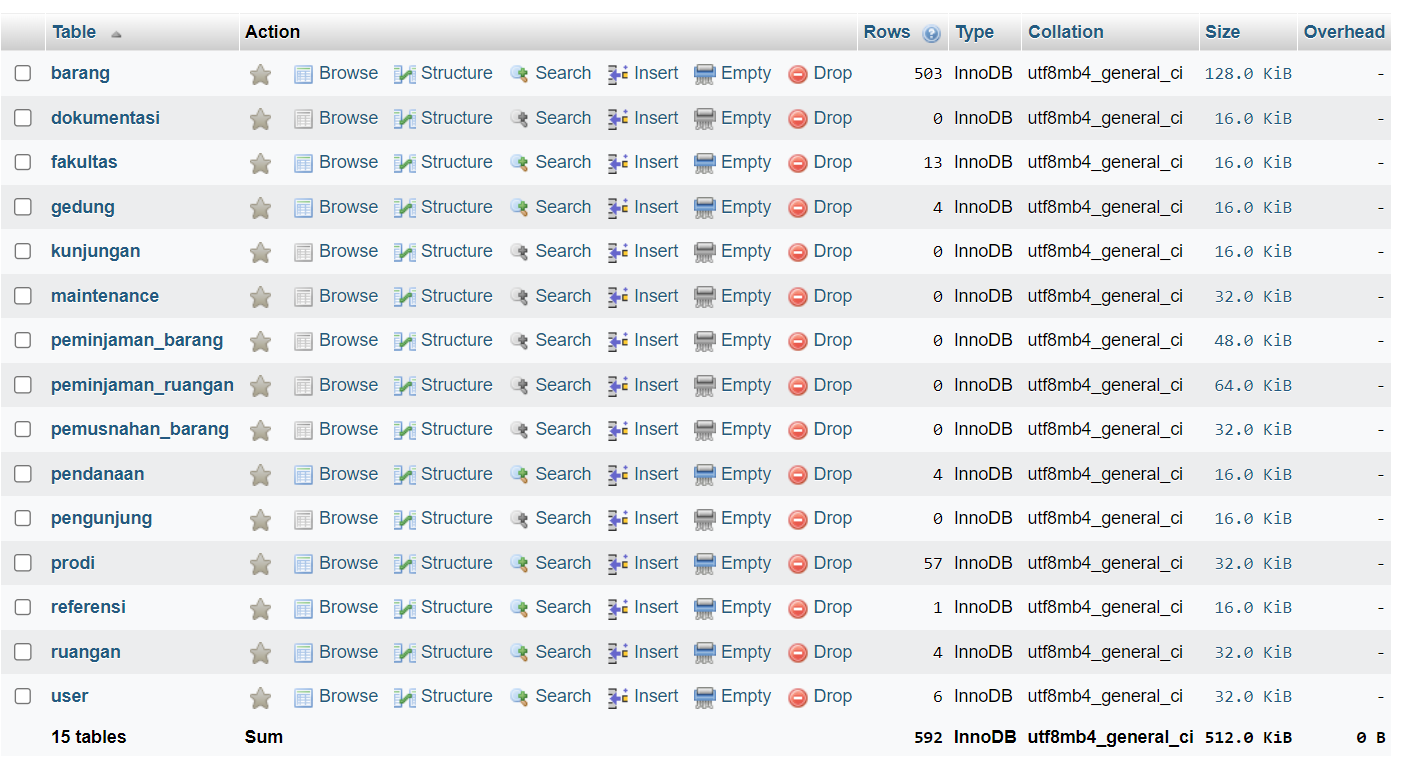
\includegraphics[width=0.82\linewidth]{konten//gambar/Tampilan tabel-tabel database.png}
          \caption{Tampilan Tabel Dalam \textit{Database}}
          \label{fig:enter-label}
        \end{figure}

  \item Struktur Tabel Barang
        Pada tabel data barang terdiri dari kolom id\_barang yang menjadi kunci utama dari tabel tersebut yang digunakan sebagai penanda agar tidak terjadi duplikasi data, id\_pendanaan menjadi kunci asing dalam tabel barang karena jenis pendanaan diperlukan dalam pencatatan data barang, id\_ruangan juga merupakan kunci asing yang diperoleh dari tabel ruangan karena nama ruangan diperlukan dalam pencatatan data barang, nama\_barang adalah kolom yang menyimpan nama barang yang dicatat, spek\_barang menjadi kolom yang menyimpan tentang spesifikasi barang yang dicatat, gambar\_barang merupakan kolom untuk menyimpan data gambar dari barang yang dicatat, tahun\_barang adalah kolom yang digunakan untuk mencatat tahun masuknya barang, kategori\_barang menjadi kolom untuk menyortir barang berdasarkan kategori, sub\_kategori menjadi kolom untuk menyortir barang berdasarkan subkategori turunan dari kategori barang, kondisi adalah kolom untuk menyimpan kondisi terakhir barang, tgl\_masuk\_barang digunakan untuk mengetahui tanggal masuknya barang atau tanggal dicatatnya barang, waktu\_input untuk mendeteksi kapan waktu dicatatnya barang, deskripsi menjelaskan lebih detail tentang barang yang dicatat, user\_input adalah kolom untuk melacak perubahan data berdasarkan siapa yang mencatat ke dalam sistem, user\_edit adalah kolom untuk melacak perubahan data berdasarkan siapa yang mengedit data dalam sistem, tgl\_edit adalah kolom untuk melacak perubahan data berdasarkan tanggal berapa data tersebut diedit. Tampilan dapat dilihat pada Gambar 4.2.

        \begin{figure}
          \centering
          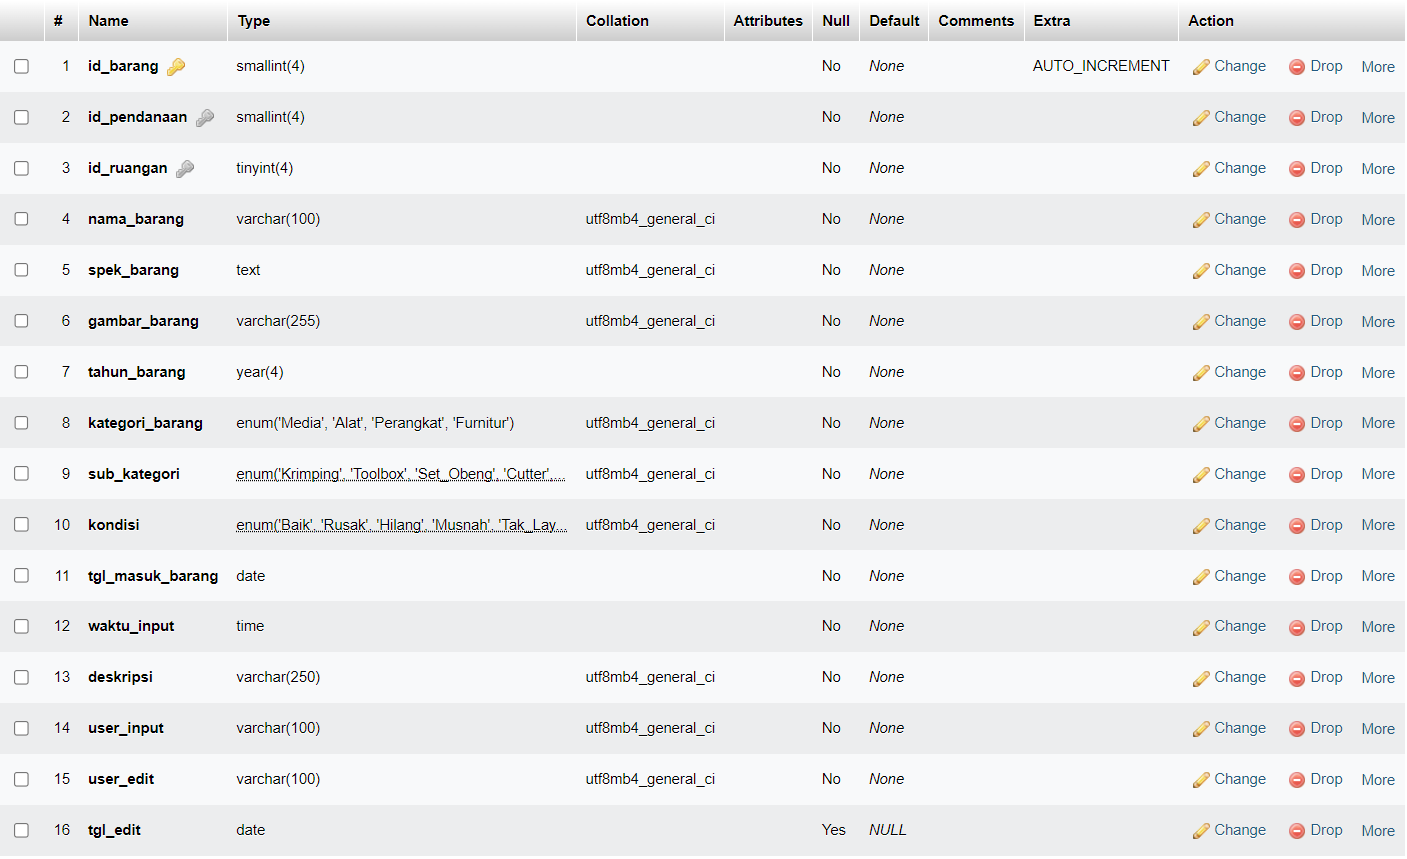
\includegraphics[width=0.82\linewidth]{konten//gambar/Tampilan database tabel barang.png}
          \caption{Tampilan \textit{Database} Tabel barang}
          \label{fig:enter-label}
        \end{figure}

  \item Struktur Tabel Dokumentasi
        Pada tabel data dokumentasi terdiri dari kolom id\_file yang menjadi kunci utama dari tabel tersebut yang digunakan sebagai penanda agar tidak terjadi duplikasi data, kategori\_dokumentasi menjadi kolom untuk menyortir dokumentasi berdasarkan kategori, nama\_dokumentasi adalah kolom yang menyimpan nama dokumentasi yang dicatat, deskripsi menjelaskan lebih detail tentang dokumentasi yang dicatat,  upload\_dokumentasi merupakan kolom untuk menyimpan data gambar atau dokumen dari dokumentasi yang dicatat, tgl\_upload digunakan untuk mengetahui tanggal diinputnya dokumentasi, waktu\_upload untuk mendeteksi kapan waktu diinputnya dokumentasi, user\_upload adalah kolom untuk melacak perubahan data berdasarkan siapa yang mencatat ke dalam sistem. Tampilan dapat dilihat pada Gambar 4.3.

        \begin{figure}
          \centering
          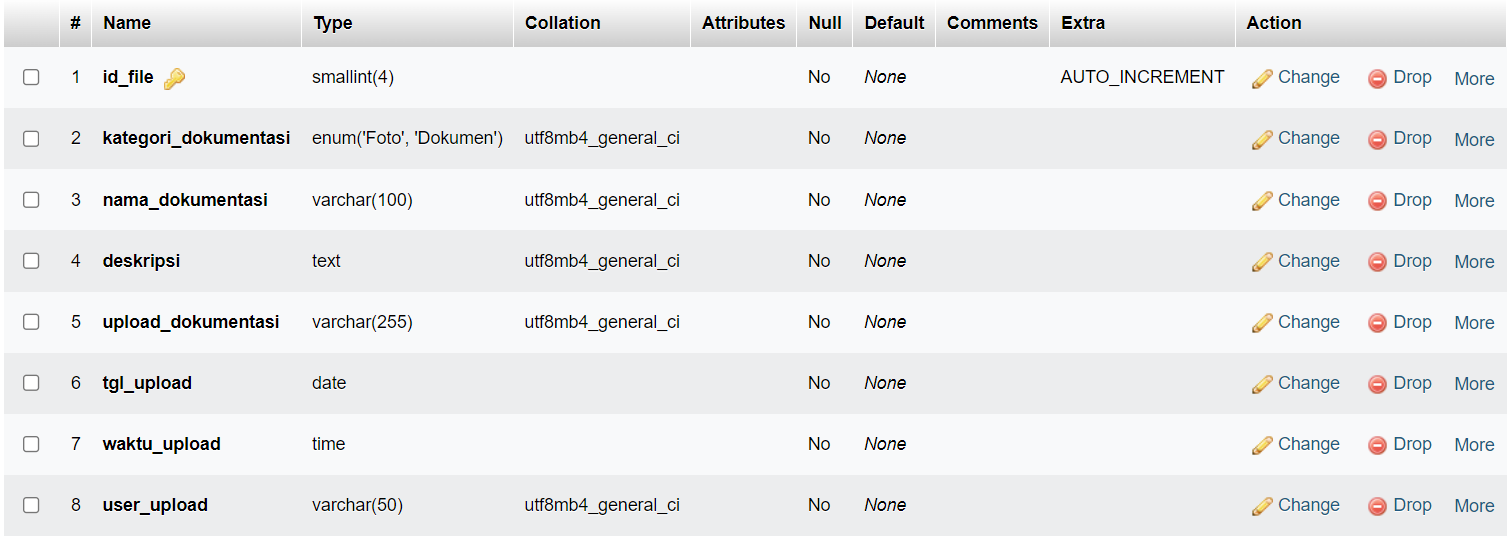
\includegraphics[width=0.82\linewidth]{konten//gambar/Tampilan database tabel dokumentasi.png}
          \caption{Tampilan \textit{Database} Tabel dokumentasi}
          \label{fig:enter-label}
        \end{figure}

  \item Struktur Tabel Fakultas
        Pada tabel data fakultas terdiri dari kolom id\_fakultas yang menjadi kunci utama dari tabel tersebut yang digunakan sebagai penanda agar tidak terjadi duplikasi data, nama\_fakultas adalah kolom yang menyimpan nama fakultas yang dicatat. Tampilan dapat dilihat pada Gambar 4.4.

        \begin{figure}
          \centering
          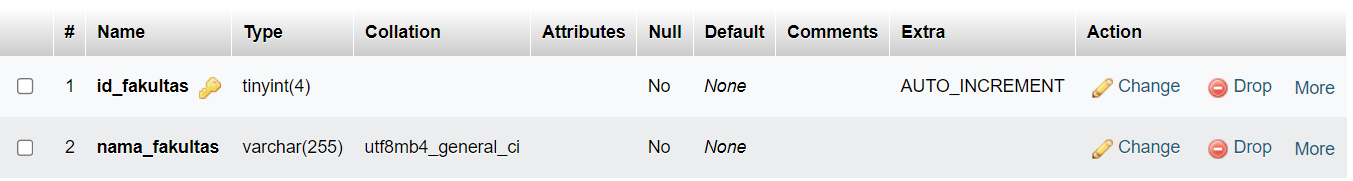
\includegraphics[width=0.82\linewidth]{konten//gambar/Tampilan database tabel fakultas.png}
          \caption{Tampilan \textit{Database} Tabel fakultas}
          \label{fig:enter-label}
        \end{figure}

  \item Struktur Tabel Gedung
        Pada tabel data gedung terdiri dari kolom id\_gedung yang menjadi kunci utama dari tabel tersebut yang digunakan sebagai penanda agar tidak terjadi duplikasi data, nama\_gedung adalah kolom yang menyimpan nama gedung yang dicatat,  deskripsi\_gedung menjelaskan lebih detail tentang gedung yang dicatat, gambar\_gedung merupakan kolom untuk menyimpan data gambar dari gedung yang dicatat. Tampilan dapat dilihat pada Gambar 4.5.

        \begin{figure}
          \centering
          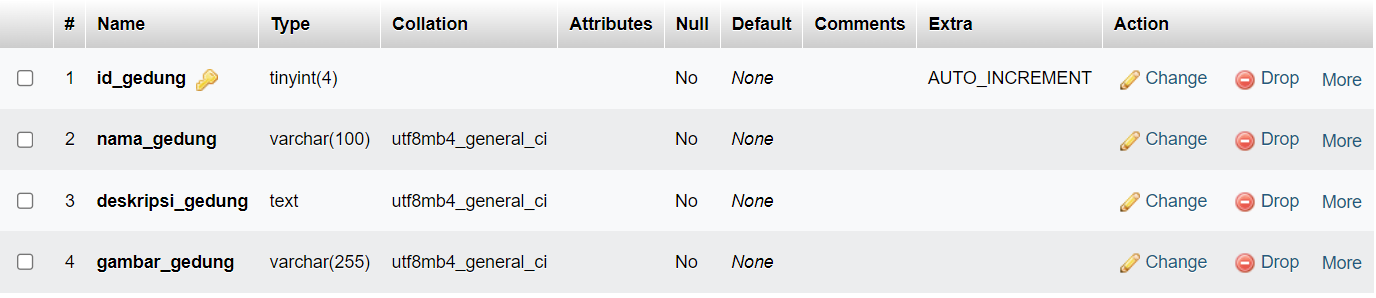
\includegraphics[width=0.82\linewidth]{konten//gambar/Tampilan database tabel gedung.png}
          \caption{Tampilan \textit{Database} Tabel gedung}
          \label{fig:enter-label}
        \end{figure}

  \item Struktur Tabel \textit{Maintenance}
        Pada tabel data \textit{maintenance} terdiri dari kolom id\_maintenance yang menjadi kunci utama dari tabel tersebut yang digunakan sebagai penanda agar tidak terjadi duplikasi data, id\_barang menjadi kunci asing dalam tabel \textit{maintenance} karena nama barang diperlukan dalam pencatatan data \textit{maintenance}, tgl\_maintenance digunakan untuk mengetahui tanggal dilakukannya \textit{maintenance} barang, kategori\_maintenance menjadi kolom untuk menyortir \textit{maintenance} berdasarkan kategori, biaya untuk menyimpan data biaya \textit{maintenance}, deskripsi menjelaskan lebih detail tentang \textit{maintenance} yang dilakukan, bukti merupakan kolom untuk menyimpan bukti \textit{maintenance} berupa gambar atau dokumen, status adalah kolom yang menyimpan data status \textit{maintenance} berupa sedang proses atau sudah selesai. Tampilan dapat dilihat pada Gambar 4.6.

        \begin{figure}
          \centering
          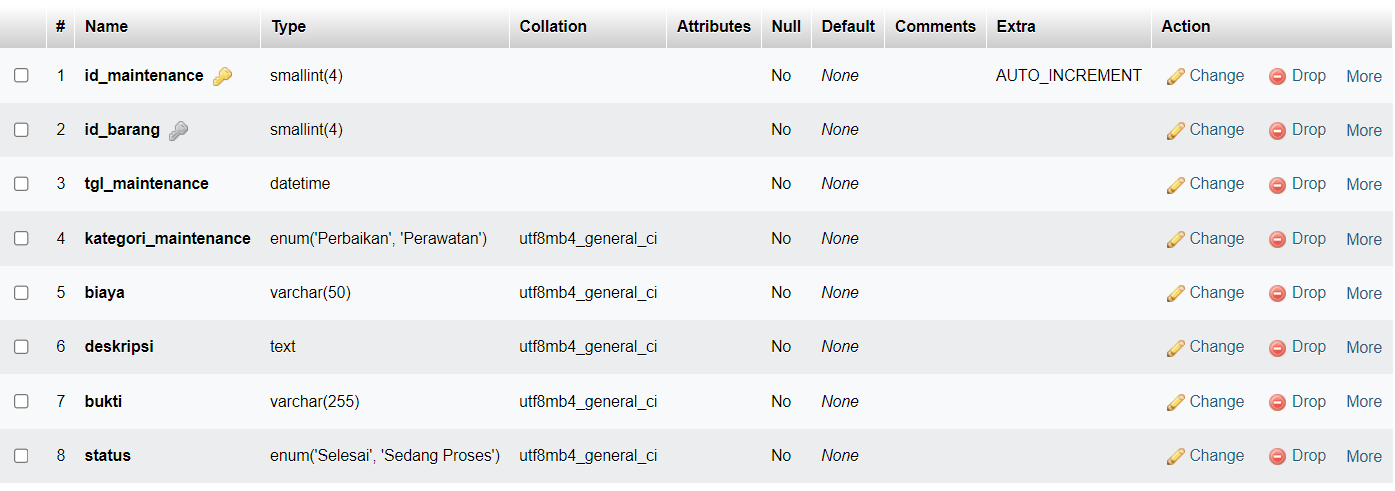
\includegraphics[width=0.82\linewidth]{konten//gambar/Tampilan database tabel maintenance.png}
          \caption{Tampilan \textit{Database} Tabel \textit{maintenance}}
          \label{fig:enter-label}
        \end{figure}

  \item Struktur Tabel Peminjaman Barang
        Pada tabel data peminjaman\_barang terdiri dari kolom id\_peminjaman\_barang yang menjadi kunci utama dari tabel tersebut yang digunakan sebagai penanda agar tidak terjadi duplikasi data, id\_barang, id\_fakultas menjadi kunci asing dalam tabel peminjaman barang karena nama fakultas diperlukan dalam pencatatan data peminjaman barang, id\_prodi menjadi kunci asing dalam tabel peminjaman barang karena nama prodi diperlukan dalam pencatatan data peminjaman barang, tgl\_peminjaman merupakan kolom untuk menyimpan tanggal barang dipinjam, tgl\_pengembalian merupakan kolom untuk menyimpan tanggal barang dikembalikan, asal\_peminjam merupakan kolom untuk membedakan antara peminjam internal dan peminjam eksternal, organisasi merupakan kolom untuk menyimpan nama organisasi dari peminjam, nama\_peminjam merupakan kolom untuk menyimpan nama dari peminjam, email\_peminjam merupakan kolom untuk menyimpan email dari peminjam, no\_hp merupakan kolom untuk menyimpan nomor telepon dari peminjam eksternal, bukti\_peminjaman merupakan kolom untuk menyimpan dokumen surat peminjaman, biaya\_peminjaman merupakan kolom untuk menampilkan biaya peminjaman pada peminjam eksternal, keterangan merupakan kolom untuk menyimpan data keperluan peminjaman yang diajukan oleh peminjam. Tampilan dapat dilihat pada Gambar 4.7.

        \begin{figure}
          \centering
          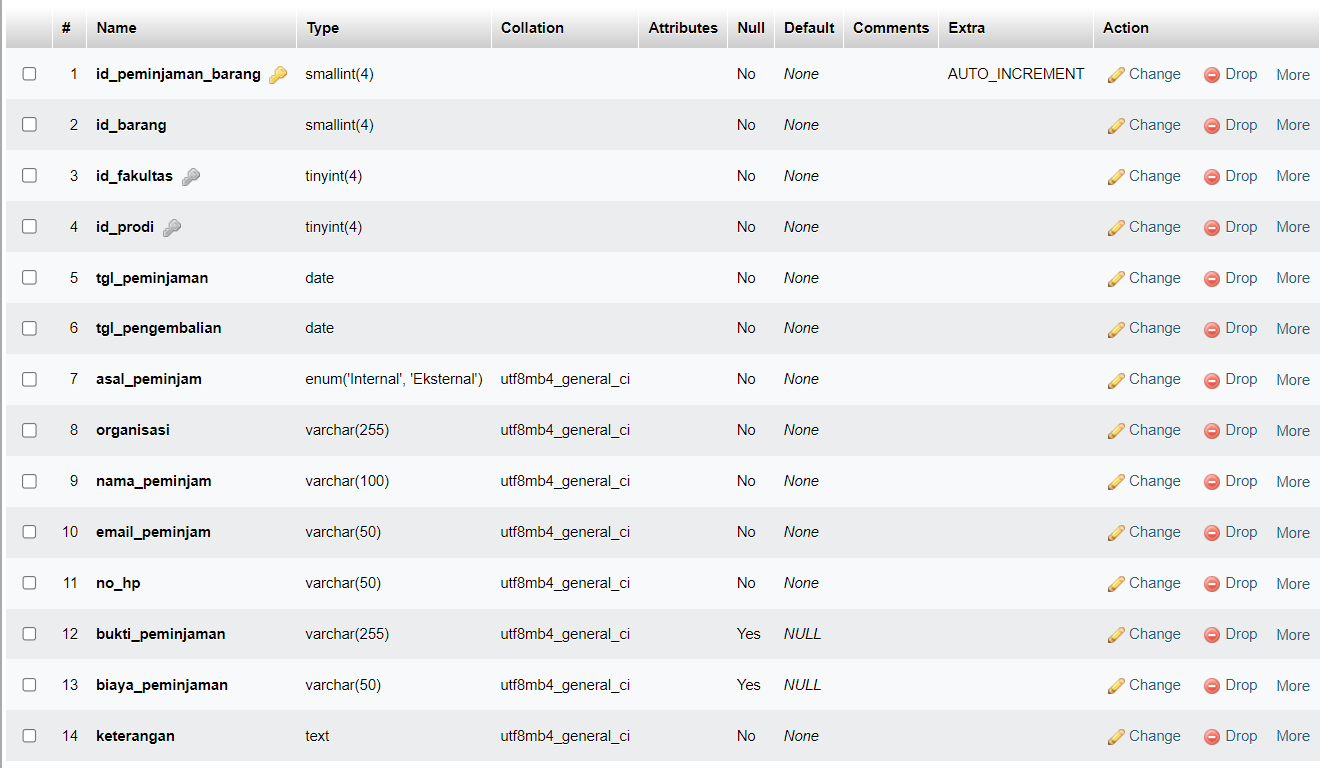
\includegraphics[width=0.82\linewidth]{konten//gambar/Tampilan database tabel peminjaman_barang.png}
          \caption{Tampilan \textit{Database} Tabel peminjaman\_barang}
          \label{fig:enter-label}
        \end{figure}

  \item Struktur Tabel Peminjaman Ruangan
        Pada tabel data peminjaman\_ruangan terdiri dari kolom id\_peminjaman\_ruangan yang menjadi kunci utama dari tabel tersebut yang digunakan sebagai penanda agar tidak terjadi duplikasi data,	id\_fakultas menjadi kunci asing dalam tabel peminjaman ruangan karena nama fakultas diperlukan dalam pencatatan data peminjaman ruangan,	id\_prodi menjadi kunci asing dalam tabel peminjaman ruangan karena nama prodi diperlukan dalam pencatatan data peminjaman ruangan,	id\_ruangan menjadi kunci asing dalam tabel peminjaman ruangan karena nama ruangan diperlukan dalam pencatatan data peminjaman ruangan yang akan dipinjam, asal\_peminjam merupakan kolom untuk membedakan antara peminjam internal dan peminjam eksternal,	organisasi merupakan kolom untuk menyimpan nama organisasi dari peminjam,	nama\_peminjam merupakan kolom untuk menyimpan nama dari peminjam, email\_peminjam merupakan kolom untuk menyimpan email dari peminjam, no\_hp merupakan kolom untuk menyimpan nomor telepon dari peminjam eksternal, tgl\_peminjaman merupakan kolom untuk menyimpan tanggal ruangan dipinjam, lama\_peminjaman merupakan kolom untuk menyimpan lama ruangan dipinjam,	biaya\_peminjaman merupakan kolom untuk menampilkan biaya peminjaman pada peminjam eksternal, bukti\_peminjaman merupakan kolom untuk menyimpan dokumen surat peminjaman, keterangan merupakan kolom untuk menyimpan data keperluan peminjaman yang diajukan oleh peminjam. Tampilan dapat dilihat pada Gambar 4.8.

        \begin{figure}
          \centering
          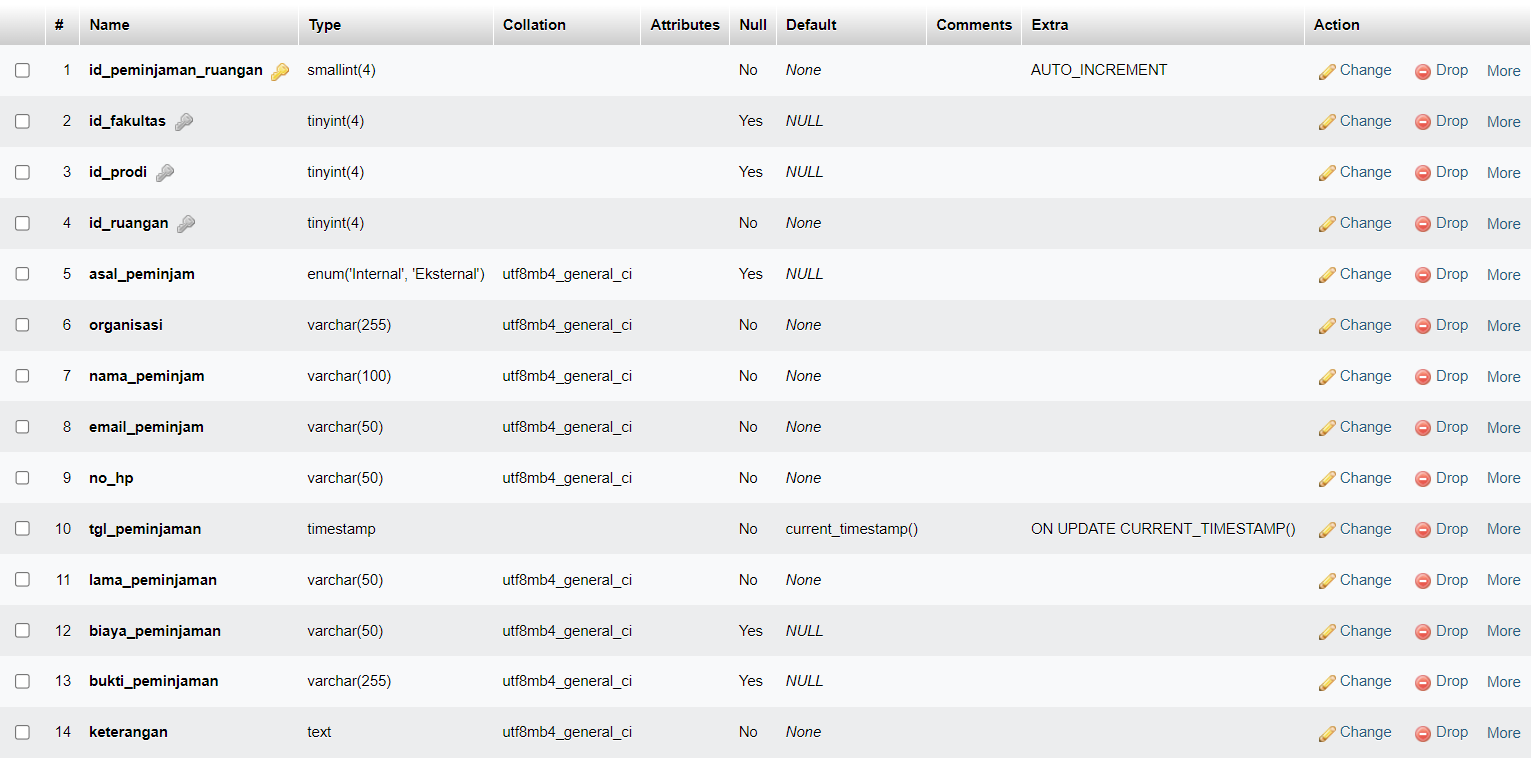
\includegraphics[width=0.82\linewidth]{konten//gambar/Tampilan database tabel peminjaman_ruangan.png}
          \caption{Tampilan \textit{Database} Tabel peminjaman\_ruangan}
          \label{fig:enter-label}
        \end{figure}

  \item Struktur Tabel Pemusnahan Barang
        Pada tabel data pemusnahan\_barang terdiri dari kolom
        id\_musnah yang menjadi kunci utama dari tabel tersebut yang digunakan sebagai penanda agar tidak terjadi duplikasi data, id\_barang menjadi kunci asing dalam tabel pemusnahan barang karena nama barang diperlukan dalam pencatatan data pemusnahan barang, tgl\_pemusnahan merupakan kolom untuk menyimpan tanggal dilakukannya pemusnahan barang, bukti\_pemusnahan merupakan kolom untuk menyimpan dokumen bukti pemusnahan, waktu untuk mendeteksi kapan waktu dimusnahkannya barang, alasan merupakan kolom untuk menyimpan alasan dilakukannya pemusnahan barang. Tampilan dapat dilihat pada Gambar 4.9.

        \begin{figure}
          \centering
          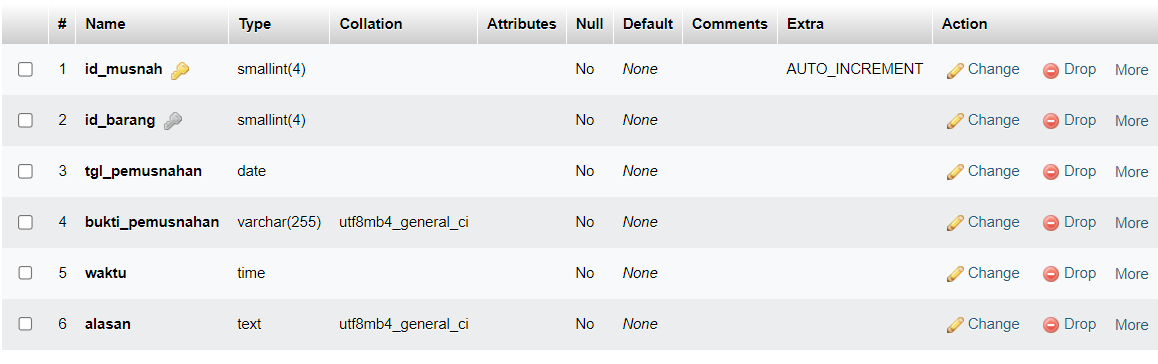
\includegraphics[width=0.82\linewidth]{konten//gambar/Tampilan database tabel pemusnahan_barang.png}
          \caption{Tampilan \textit{Database} Tabel pemusnahan\_barang}
          \label{fig:enter-label}
        \end{figure}

  \item Struktur Tabel Pendanaan
        Pada tabel data pendanaan terdiri dari kolom id\_pendanaan yang menjadi kunci utama dari tabel tersebut yang digunakan sebagai penanda agar tidak terjadi duplikasi data, jenis\_pendanaan merupakan kolom untuk menyimpan apa jenis pendanaannya, keterangan merupakan kolom untuk menyimpan data keterangan dari pendanaan. Tampilan dapat dilihat pada Gambar 4.10.

        \begin{figure}
          \centering
          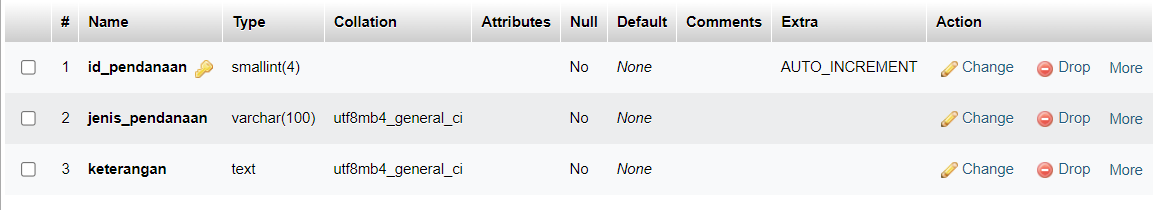
\includegraphics[width=0.82\linewidth]{konten//gambar/Tampilan database tabel pendanaan.png}
          \caption{Tampilan \textit{Database} Tabel pendanaan}
          \label{fig:enter-label}
        \end{figure}

  \item Struktur Tabel Prodi
        Pada tabel data prodi terdiri dari kolom id\_prodi yang menjadi kunci utama dari tabel tersebut yang digunakan sebagai penanda agar tidak terjadi duplikasi data, id\_fakultas menjadi kunci asing dalam tabel prodi karena nama fakultas diperlukan dalam pencatatan data prodi, nama\_prodi merupakan kolom untuk mencatat nama prodi. Tampilan dapat dilihat pada Gambar 4.11.

        \begin{figure}
          \centering
          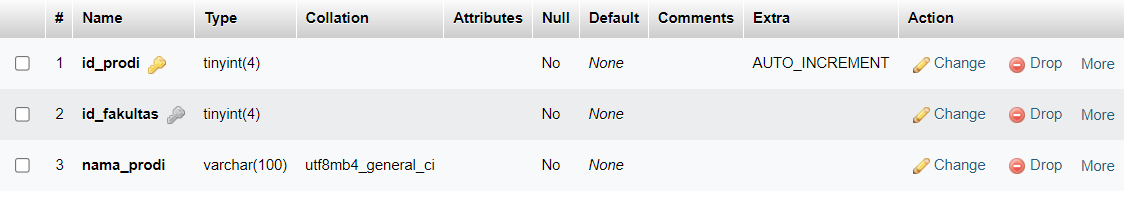
\includegraphics[width=0.82\linewidth]{konten//gambar/Tampilan database tabel prodi.png}
          \caption{Tampilan \textit{Database} Tabel prodi}
          \label{fig:enter-label}
        \end{figure}

  \item Struktur Tabel Referensi
        Pada tabel data referensi terdiri dari kolom id\_referensi yang menjadi kunci utama dari tabel tersebut yang digunakan sebagai penanda agar tidak terjadi duplikasi data, biaya kolom untuk menampilkan biaya peminjaman pada peminjam eksternal yang digunakan pada tabel peminjaman barang dan peminjaman ruangan. Tampilan dapat dilihat pada Gambar 4.12.

        \begin{figure}
          \centering
          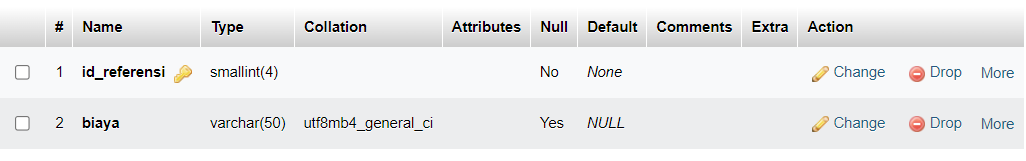
\includegraphics[width=0.82\linewidth]{konten//gambar/Tampilan database tabel referensi.png}
          \caption{Tampilan \textit{Database} Tabel referensi}
          \label{fig:enter-label}
        \end{figure}

  \item Struktur Tabel Ruangan
        Pada tabel data ruangan terdiri dari kolom id\_ruangan yang menjadi kunci utama dari tabel tersebut yang digunakan sebagai penanda agar tidak terjadi duplikasi data, id\_gedung menjadi kunci asing dalam tabel ruangan karena nama gedung diperlukan dalam pencatatan data ruangan, nama\_ruangan adalah kolom yang menyimpan nama ruangan yang dicatat, deskripsi\_ruangan menjelaskan detail tentang ruangan yang dicatat, gambar\_ruangan merupakan kolom untuk menyimpan data gambar dari ruangan yang dicatat. Tampilan dapat dilihat pada Gambar 4.13.

        \begin{figure}
          \centering
          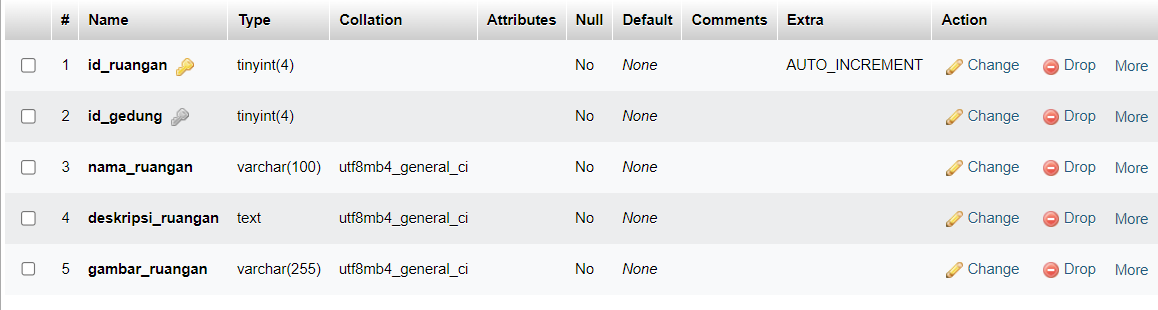
\includegraphics[width=0.82\linewidth]{konten//gambar/Tampilan database tabel ruangan.png}
          \caption{Tampilan \textit{Database} Tabel ruangan}
          \label{fig:enter-label}
        \end{figure}

  \item Struktur Tabel User
        Pada tabel data user terdiri dari kolom id\_user yang menjadi kunci utama dari tabel tersebut yang digunakan sebagai penanda agar tidak terjadi duplikasi data, nama merupakan kolom yang menyimpan nama pengguna, foto merupakan kolom untuk menyimpan foto profil pengguna, no\_identitas merupakan kolom yang digunakan untuk menyimpan data NIM, NIP, atau NIK dari pengguna, \textit{username} merupakan kolom yang digunakan untuk menyimpan \textit{username} pengguna, password\_hash merupakan kolom yang digunakan untuk menyimpan \textit{password} pengguna, email merupakan kolom yang digunakan untuk menyimpan email pengguna, role\_user merupakan kolom yang digunakan untuk menyimpan level akses pengguna. Tampilan dapat dilihat pada Gambar 4.14.

        \begin{figure}
          \centering
          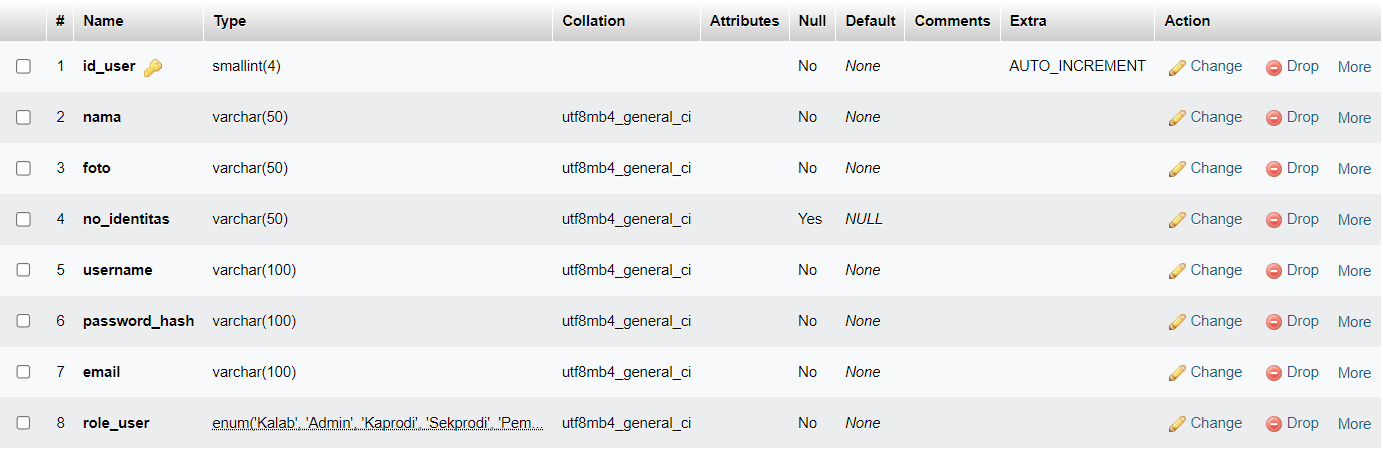
\includegraphics[width=0.82\linewidth]{konten//gambar/Tampilan database tabel user.png}
          \caption{Tampilan \textit{Database} Tabel user}
          \label{fig:enter-label}
        \end{figure}

\end{enumerate}

% -----------------------------------------------------------------------------%
\section{Implementasi Kode Pemrograman}
\subsection{\textit{Routes}}
\textit{Routes} dalam konsep MVC \textit{(Model-View-Controller)} adalah mekanisme yang digunakan untuk mengatur bagaimana permintaan (\textit{requests}) dari pengguna atau klien akan ditangani oleh aplikasi web. \textit{Routes} menentukan hubungan antara URL yang diminta oleh pengguna dengan \textit{controller} yang akan menangani permintaan tersebut \cite{kelvin2022sistem}.

\begin{enumerate}
  \item \textit{Routes} dalam implementasi sistem informasi inventaris laboratorium pada data barang dapat dilihat pada Gambar 4.15.

        \begin{figure}
          \centering
          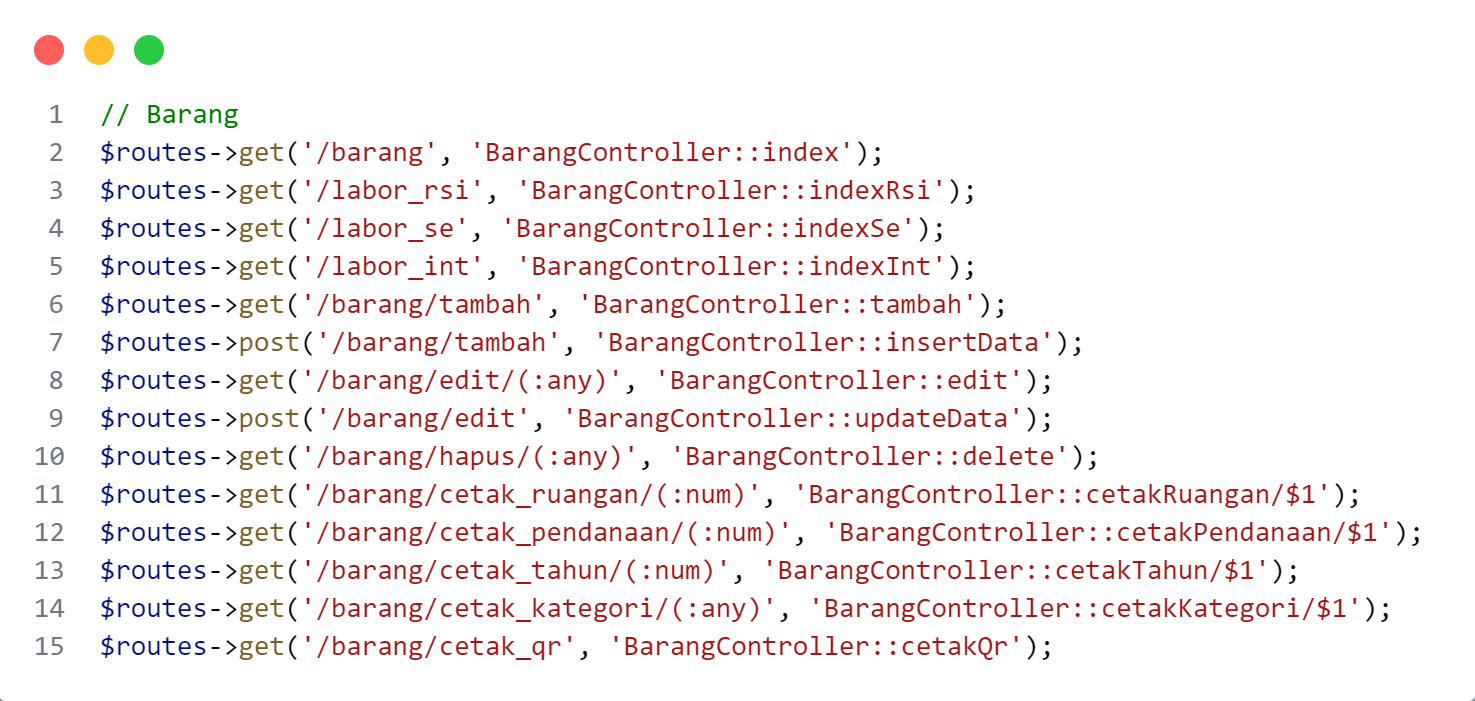
\includegraphics[width=0.82\linewidth]{konten//gambar/routes barang.png}
          \caption{\textit{Routes} Barang}
          \label{fig:enter-label}
        \end{figure}

  \item \textit{Routes} dalam implementasi sistem informasi inventaris laboratorium pada data dokumentasi dapat dilihat pada Gambar 4.16.

        \begin{figure}
          \centering
          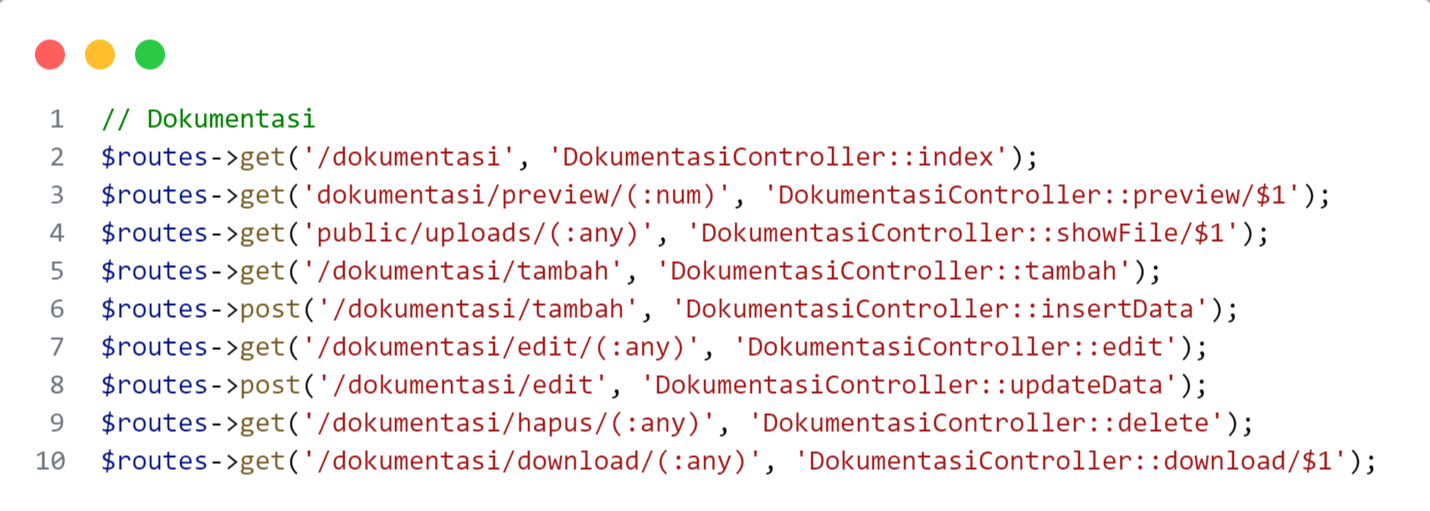
\includegraphics[width=0.82\linewidth]{konten//gambar/routes dokumentasi.png}
          \caption{\textit{Routes} Dokumentasi}
          \label{fig:enter-label}
        \end{figure}

  \item \textit{Routes} dalam implementasi sistem informasi inventaris laboratorium pada data fakultas dapat dilihat pada Gambar 4.17.

        \begin{figure}
          \centering
          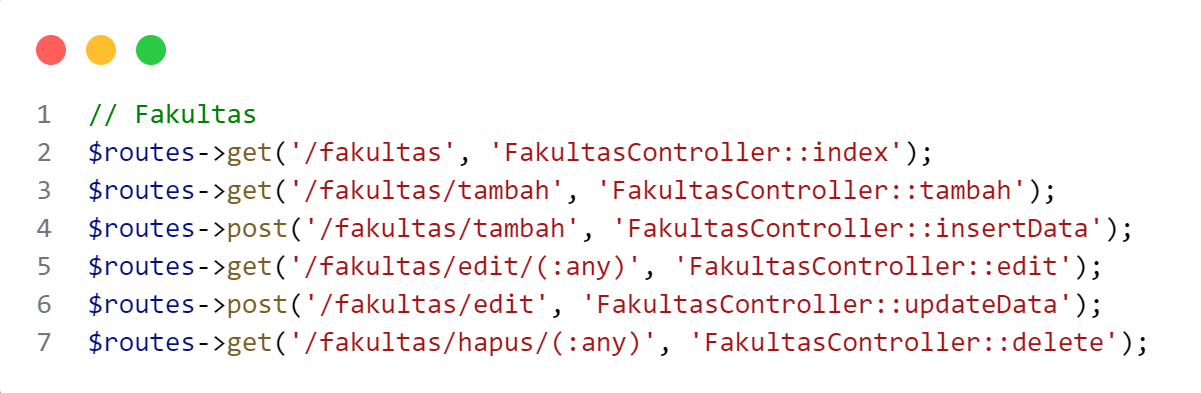
\includegraphics[width=0.82\linewidth]{konten//gambar/routes fakultas.png}
          \caption{\textit{Routes} Fakultas}
          \label{fig:enter-label}
        \end{figure}

  \item \textit{Routes} dalam implementasi sistem informasi inventaris laboratorium pada data gedung dapat dilihat pada Gambar 4.18.

        \begin{figure}
          \centering
          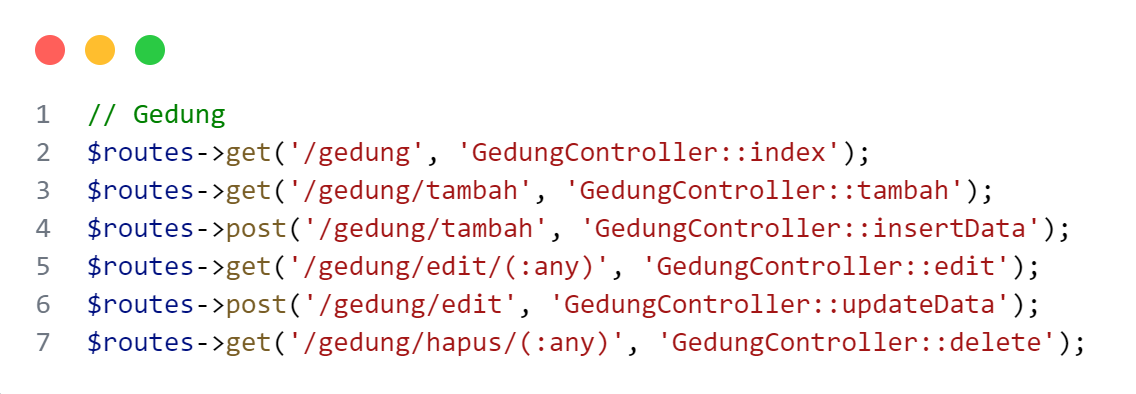
\includegraphics[width=0.82\linewidth]{konten//gambar/routes gedung.png}
          \caption{\textit{Routes} Gedung}
          \label{fig:enter-label}
        \end{figure}

  \item \textit{Routes} dalam implementasi sistem informasi inventaris laboratorium pada data \textit{maintenance} dapat dilihat pada Gambar 4.19.

        \begin{figure}
          \centering
          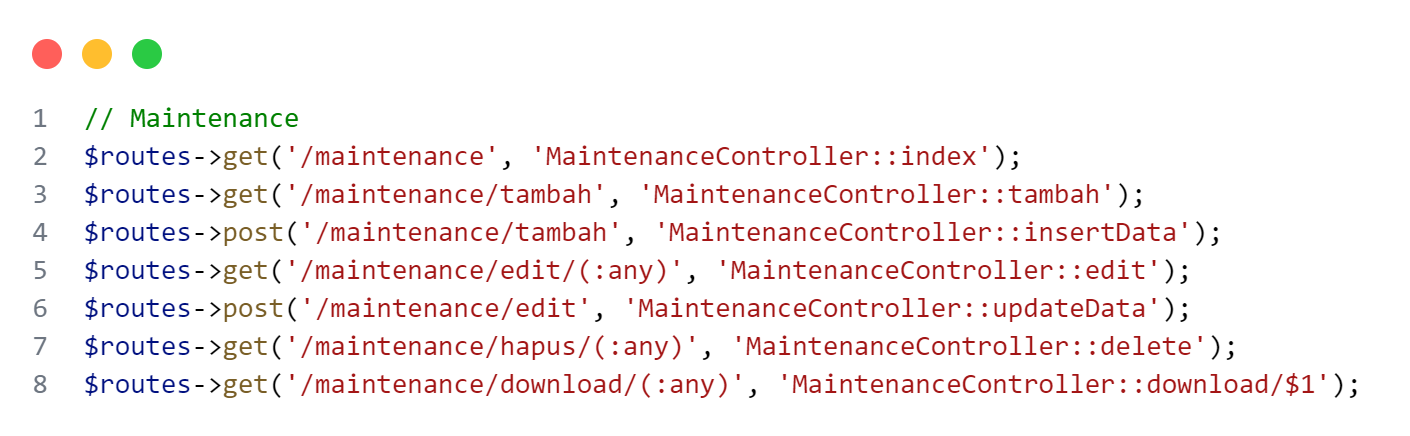
\includegraphics[width=0.82\linewidth]{konten//gambar/routes maintenance.png}
          \caption{\textit{Routes Maintenance}}
          \label{fig:enter-label}
        \end{figure}

  \item \textit{Routes} dalam implementasi sistem informasi inventaris laboratorium pada data peminjaman barang dapat dilihat pada Gambar 4.20.

        \begin{figure}
          \centering
          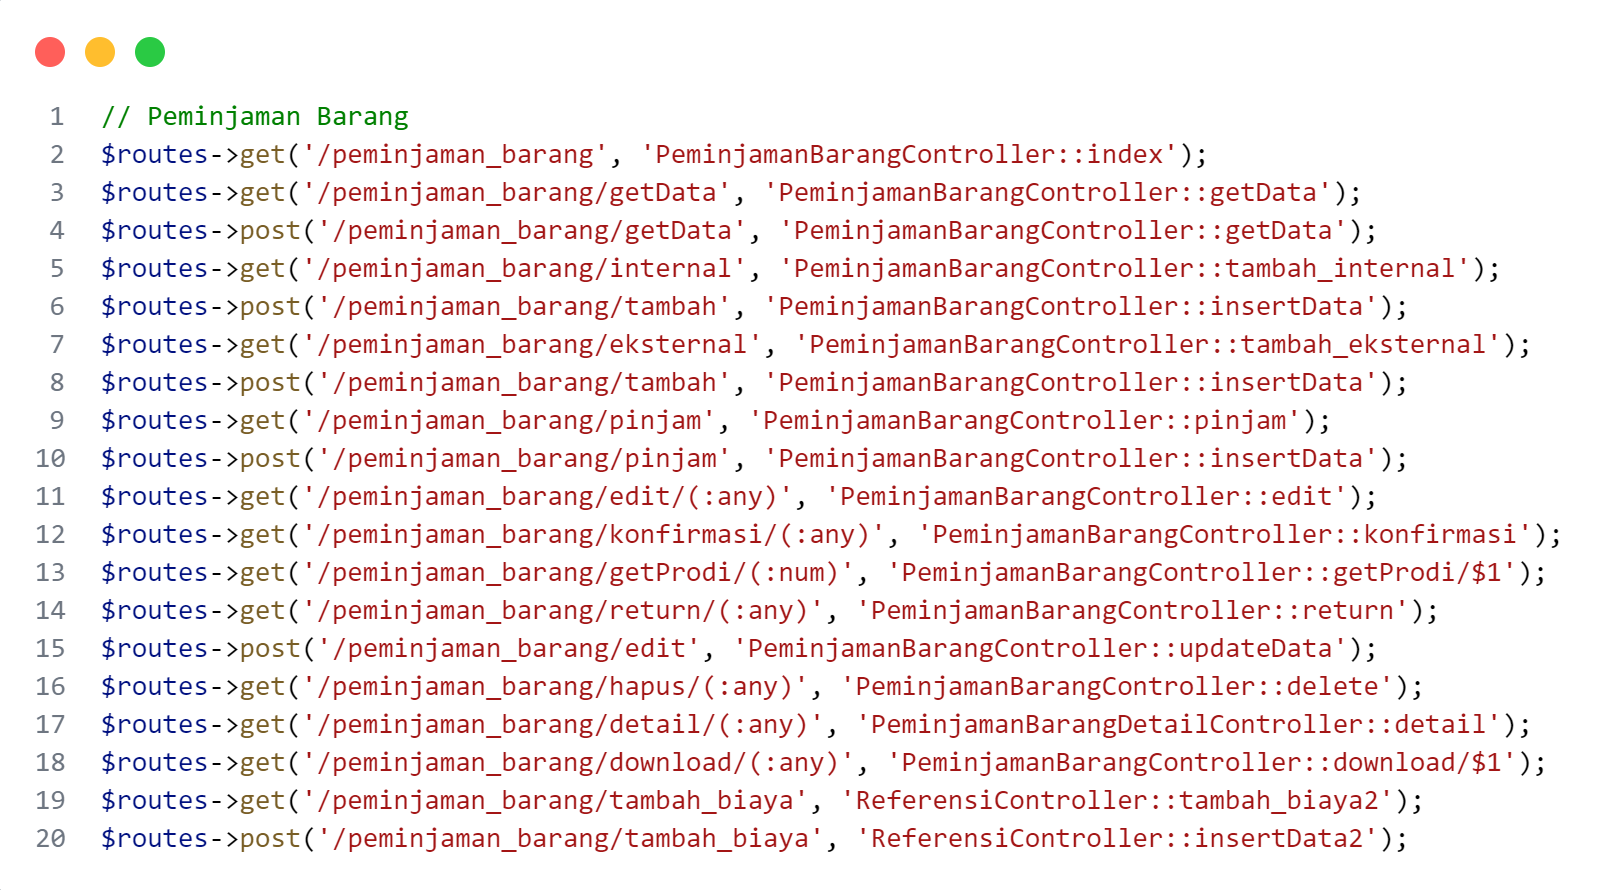
\includegraphics[width=0.82\linewidth]{konten//gambar/routes peminjaman barang.png}
          \caption{\textit{Routes} Peminjaman Barang}
          \label{fig:enter-label}
        \end{figure}

  \item \textit{Routes} dalam implementasi sistem informasi inventaris laboratorium pada data peminjaman ruangan dapat dilihat pada Gambar 4.21.

        \begin{figure}
          \centering
          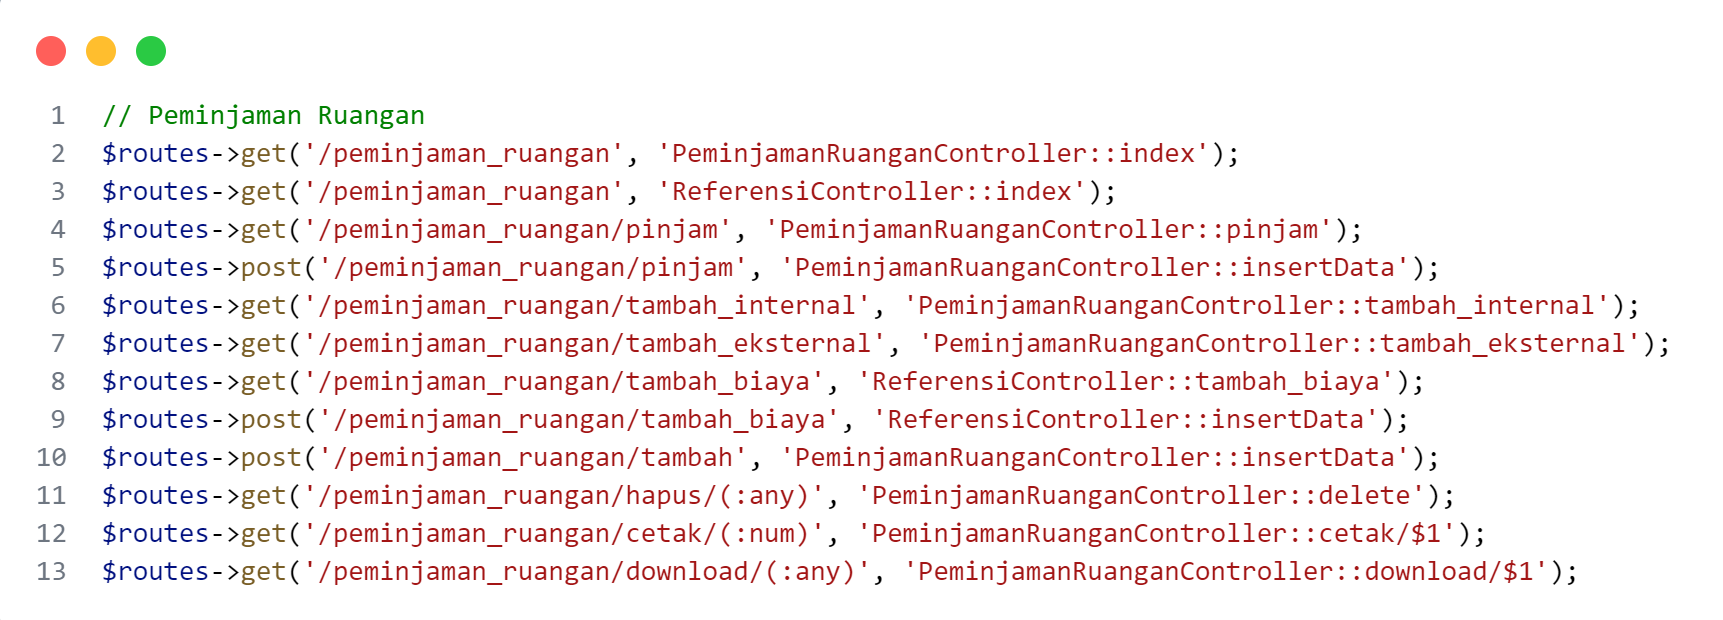
\includegraphics[width=0.82\linewidth]{konten//gambar/routes peminjaman ruangan.png}
          \caption{\textit{Routes} Peminjaman Ruangan}
          \label{fig:enter-label}
        \end{figure}

  \item \textit{Routes} dalam implementasi sistem informasi inventaris laboratorium pada data pemusnahan barang dapat dilihat pada Gambar 4.22.

        \begin{figure}
          \centering
          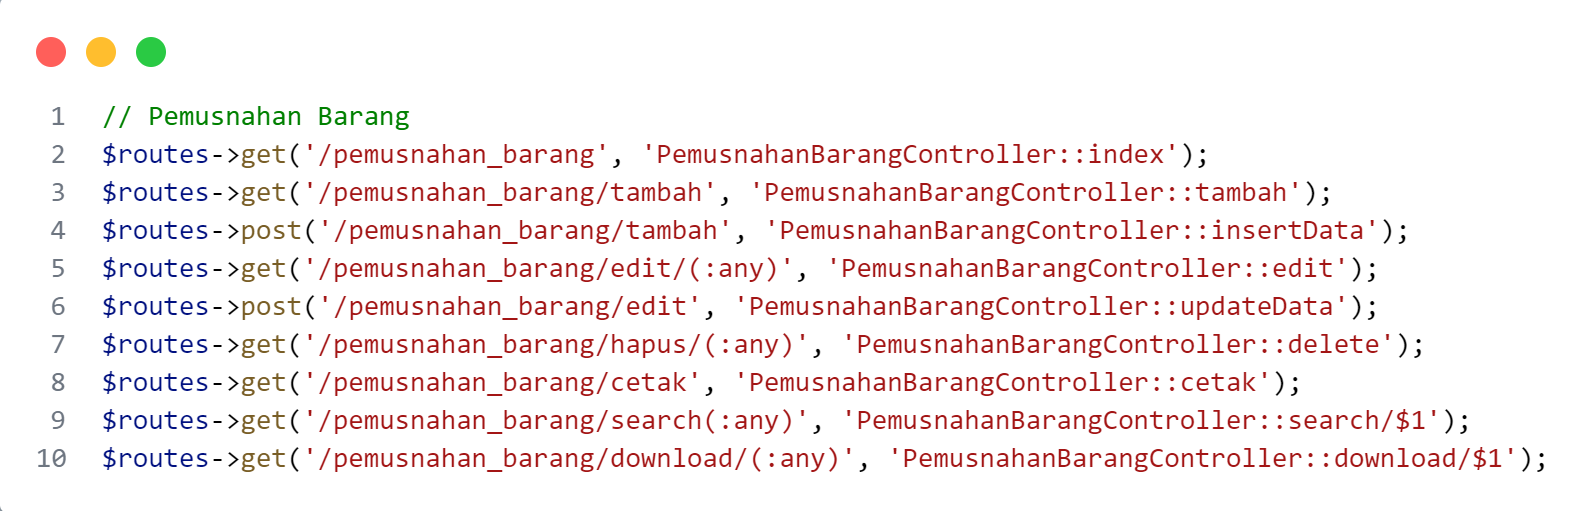
\includegraphics[width=0.82\linewidth]{konten//gambar/routes pemusnahan barang.png}
          \caption{\textit{Routes} Pemusnahan Barang}
          \label{fig:enter-label}
        \end{figure}

  \item \textit{Routes} dalam implementasi sistem informasi inventaris laboratorium pada data pendanaan dapat dilihat pada Gambar 4.23.

        \begin{figure}
          \centering
          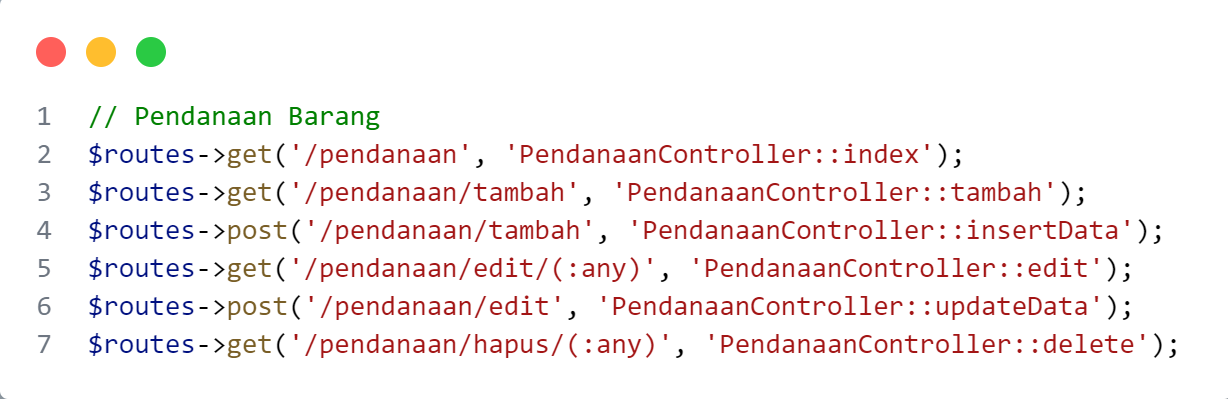
\includegraphics[width=0.82\linewidth]{konten//gambar/routes pendanaan.png}
          \caption{\textit{Routes} Pendanaan}
          \label{fig:enter-label}
        \end{figure}

  \item \textit{Routes} dalam implementasi sistem informasi inventaris laboratorium pada data prodi dapat dilihat pada Gambar 4.24.

        \begin{figure}
          \centering
          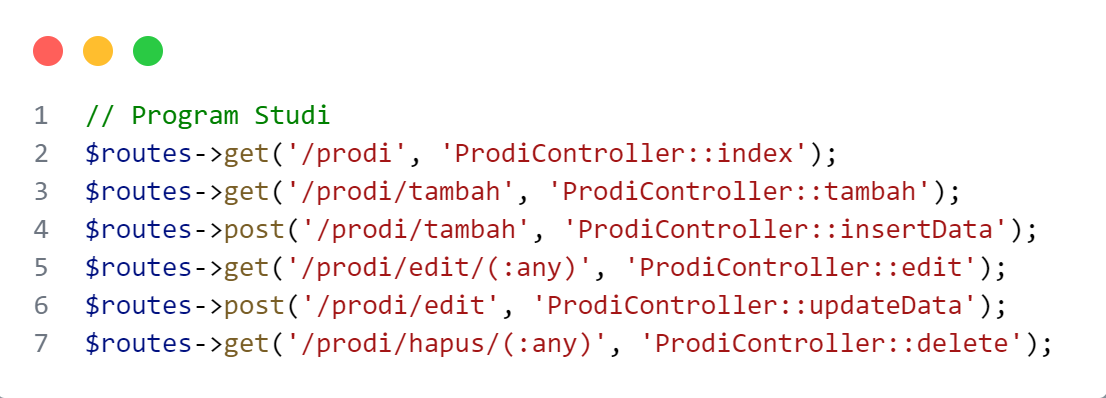
\includegraphics[width=0.82\linewidth]{konten//gambar/routes prodi.png}
          \caption{\textit{Routes} Prodi}
          \label{fig:enter-label}
        \end{figure}

  \item \textit{Routes} dalam implementasi sistem informasi inventaris laboratorium pada data ruangan dapat dilihat pada Gambar 4.25.

        \begin{figure}
          \centering
          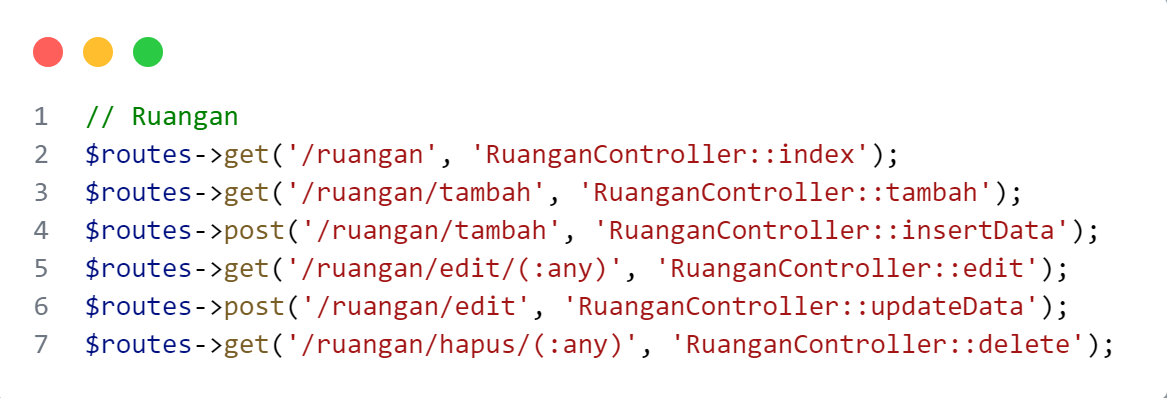
\includegraphics[width=0.82\linewidth]{konten//gambar/routes ruangan.png}
          \caption{\textit{Routes} Ruangan}
          \label{fig:enter-label}
        \end{figure}

  \item \textit{Routes} dalam implementasi sistem informasi inventaris laboratorium pada data \textit{user} dapat dilihat pada Gambar 4.26.

        \begin{figure}
          \centering
          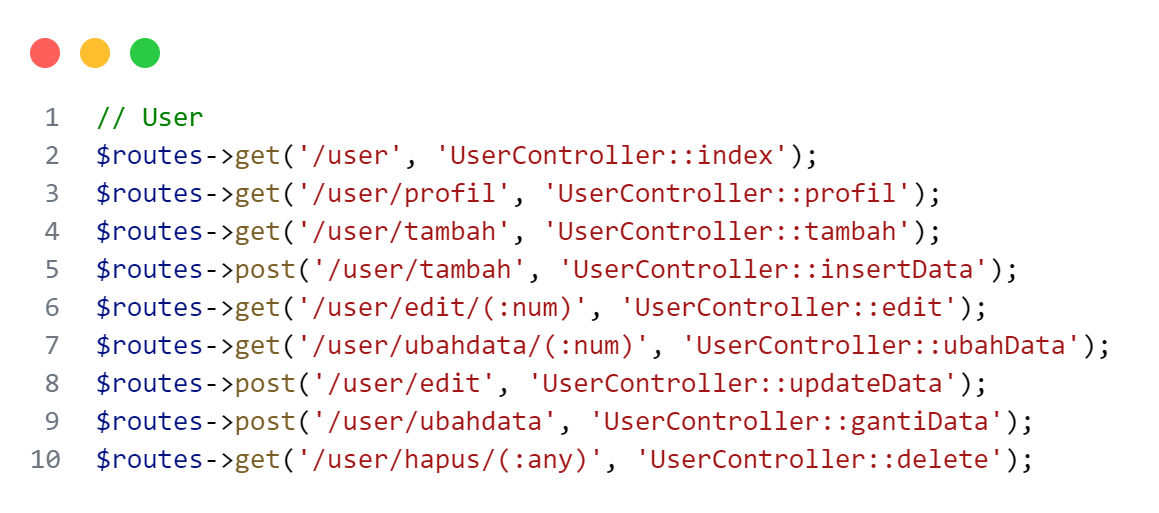
\includegraphics[width=0.82\linewidth]{konten//gambar/routes user.png}
          \caption{\textit{Routes} \textit{User}}
          \label{fig:enter-label}
        \end{figure}
\end{enumerate}

\subsection{Model}
Model adalah komponen yang bertanggung jawab untuk mengatur data, aturan bisnis, dan logika aplikasi. Ini merupakan representasi dari data dalam aplikasi. Model mengelola semua operasi data, seperti pengambilan, pembaruan, dan penyimpanan data \cite{firdaus2020rancang}.

\begin{enumerate}
  \item Model dalam implementasi sistem informasi inventaris laboratorium pada data barang dapat dilihat pada Gambar 4.27.

        \begin{figure}
          \centering
          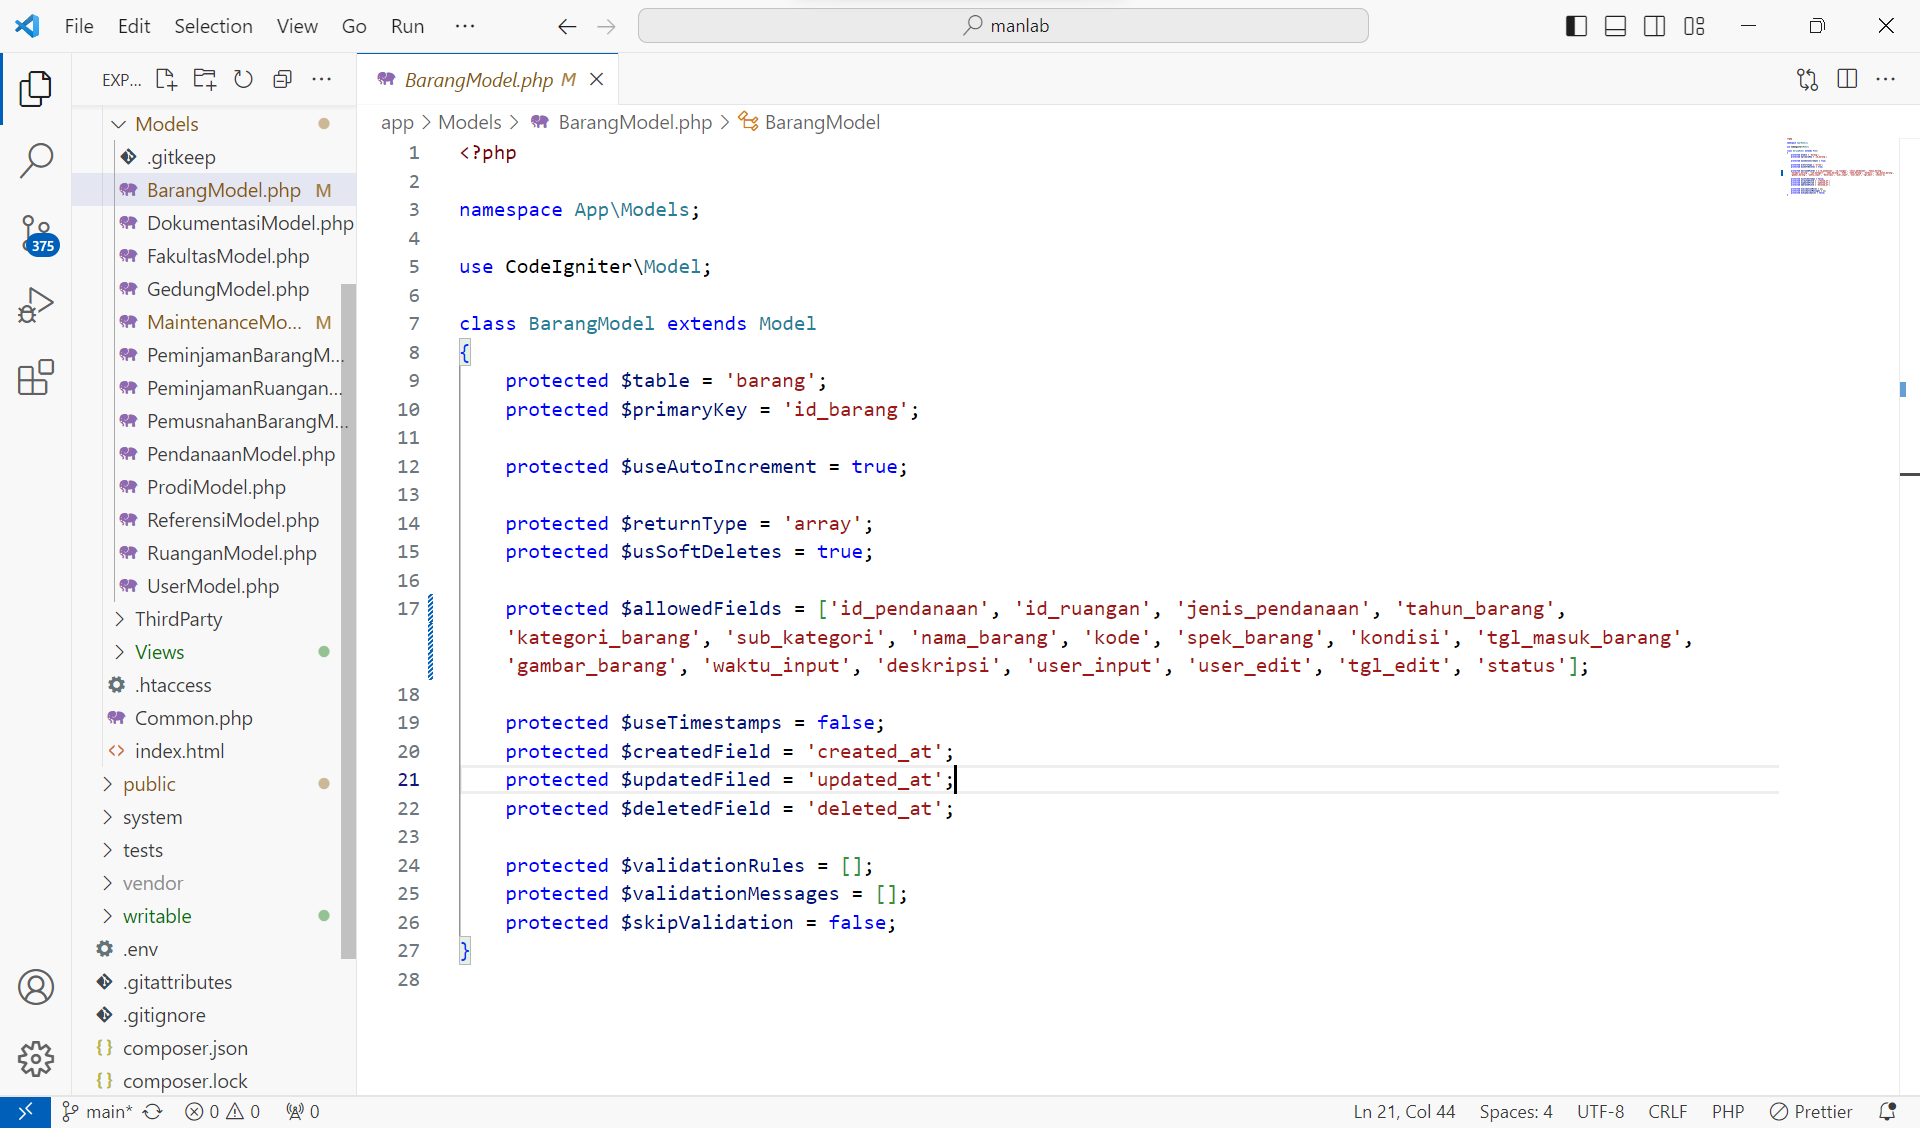
\includegraphics[width=0.82\linewidth]{konten//gambar/barang model.png}
          \caption{Model Barang}
          \label{fig:enter-label}
        \end{figure}

  \item Model dalam implementasi sistem informasi inventaris laboratorium pada data dokumentasi dapat dilihat pada Gambar 4.28.

        \begin{figure}
          \centering
          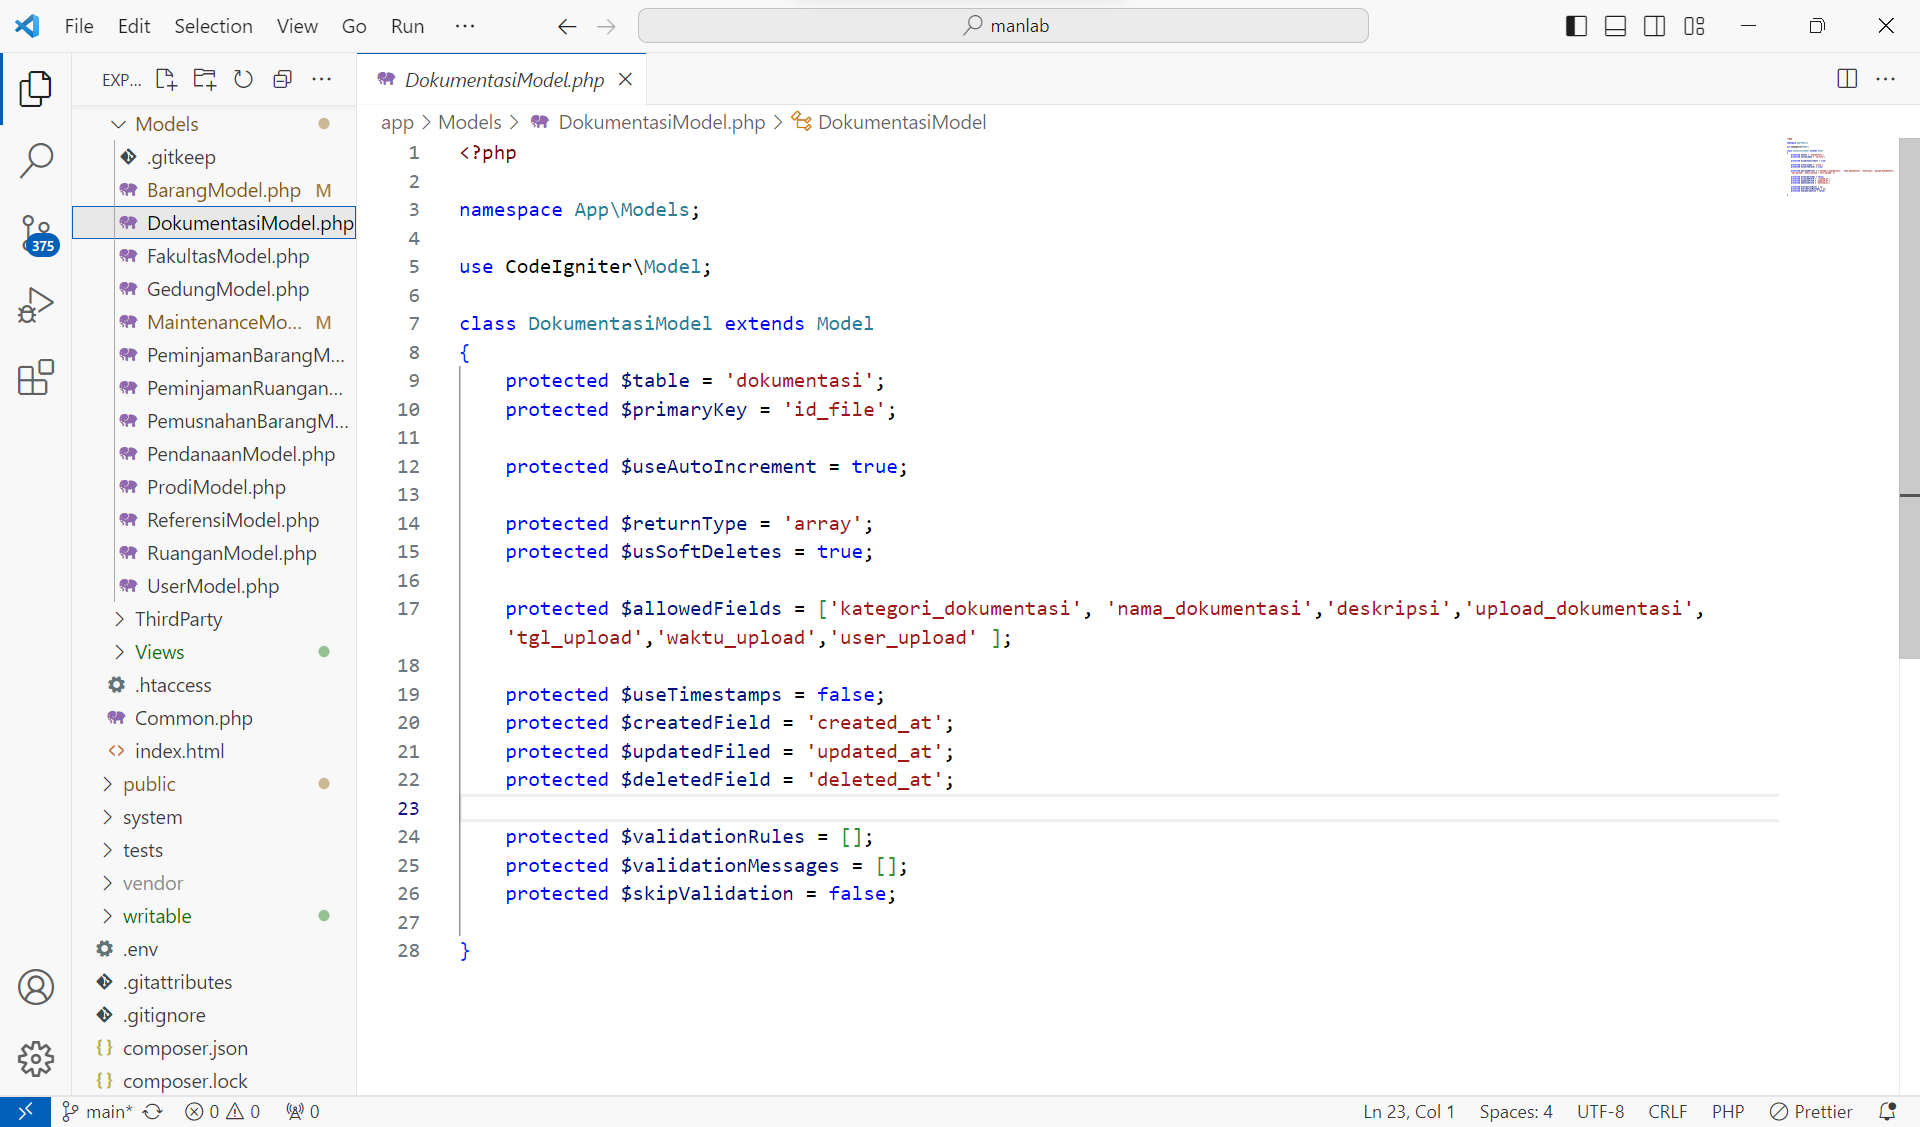
\includegraphics[width=0.82\linewidth]{konten//gambar/dokumentasi model.png}
          \caption{Model Dokumentasi}
          \label{fig:enter-label}
        \end{figure}

  \item Model dalam implementasi sistem informasi inventaris laboratorium pada data fakultas dapat dilihat pada Gambar 4.29.

        \begin{figure}
          \centering
          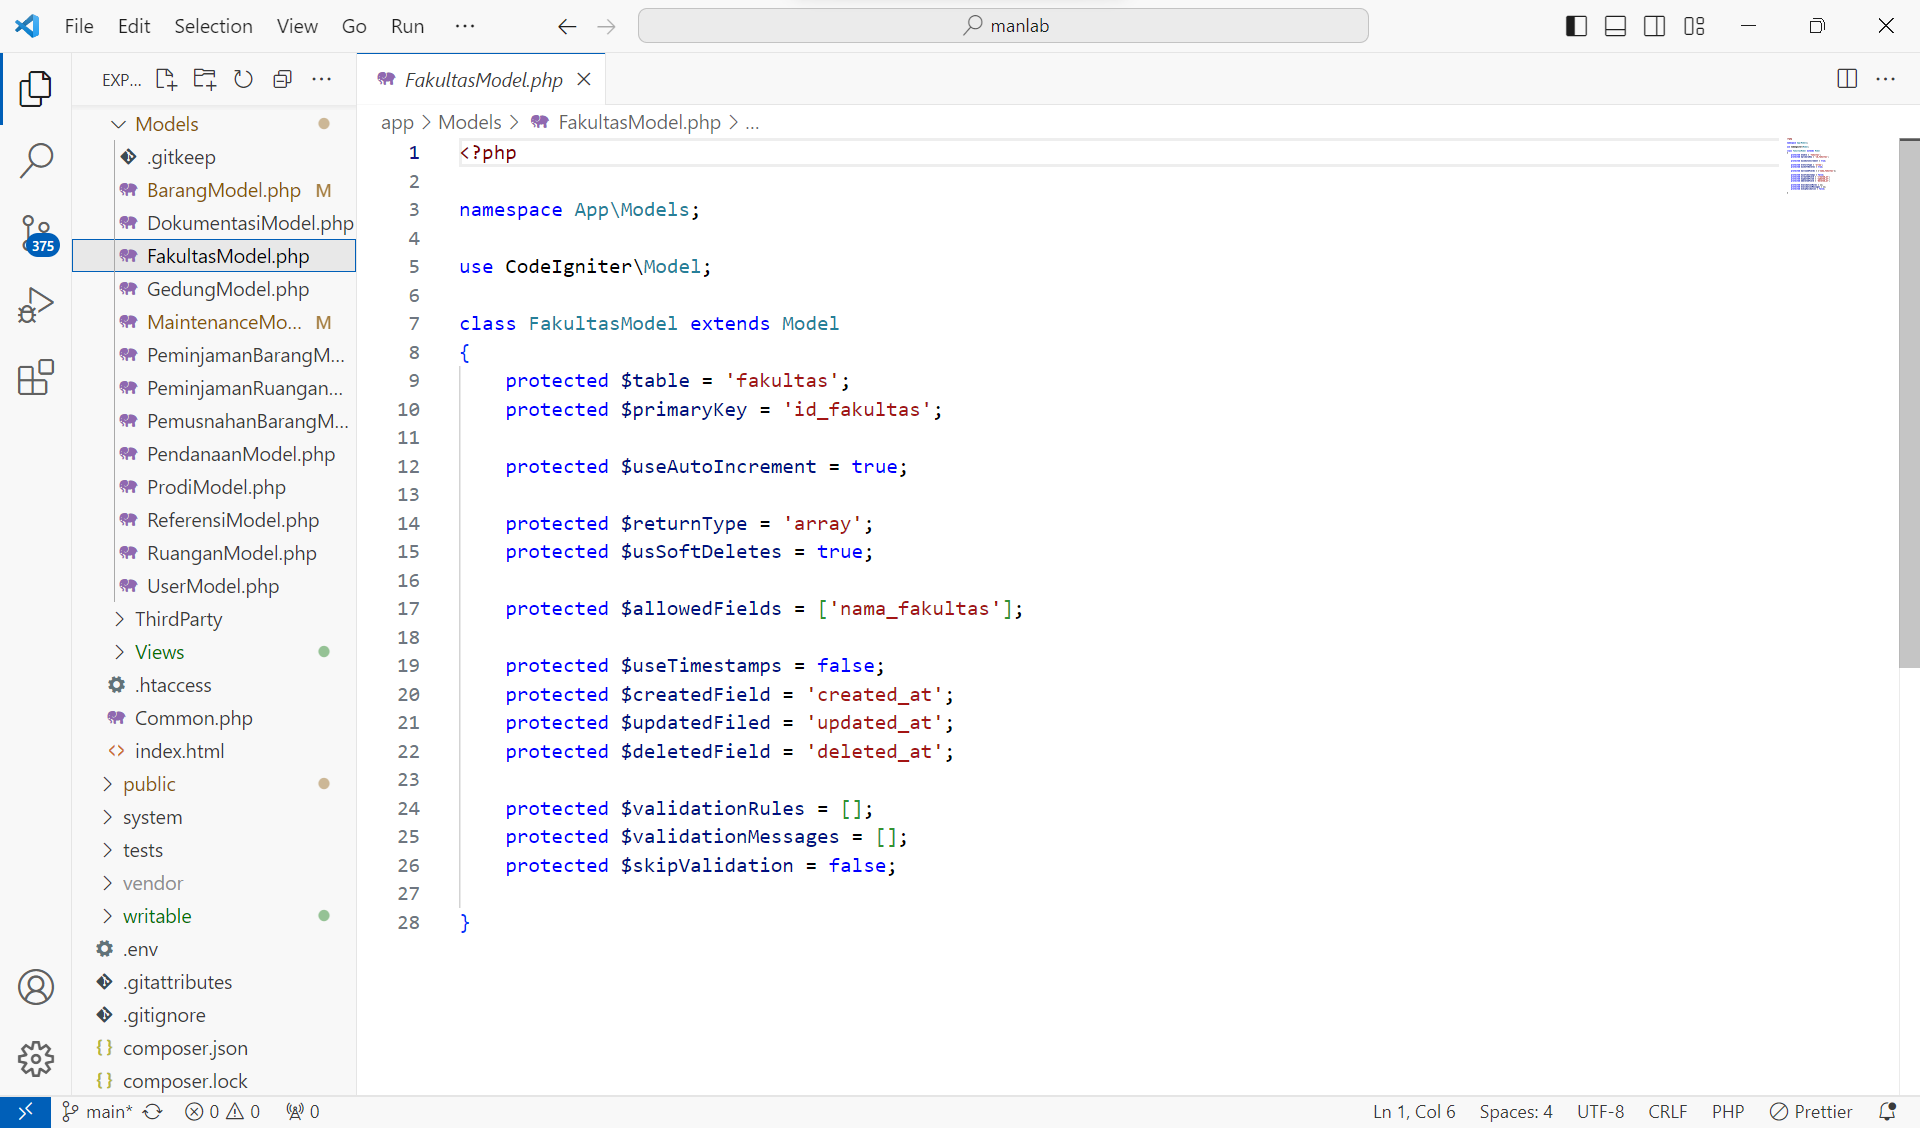
\includegraphics[width=0.82\linewidth]{konten//gambar/fakultas model.png}
          \caption{Model Fakultas}
          \label{fig:enter-label}
        \end{figure}

  \item Model dalam implementasi sistem informasi inventaris laboratorium pada data gedung dapat dilihat pada Gambar 4.30.

        \begin{figure}
          \centering
          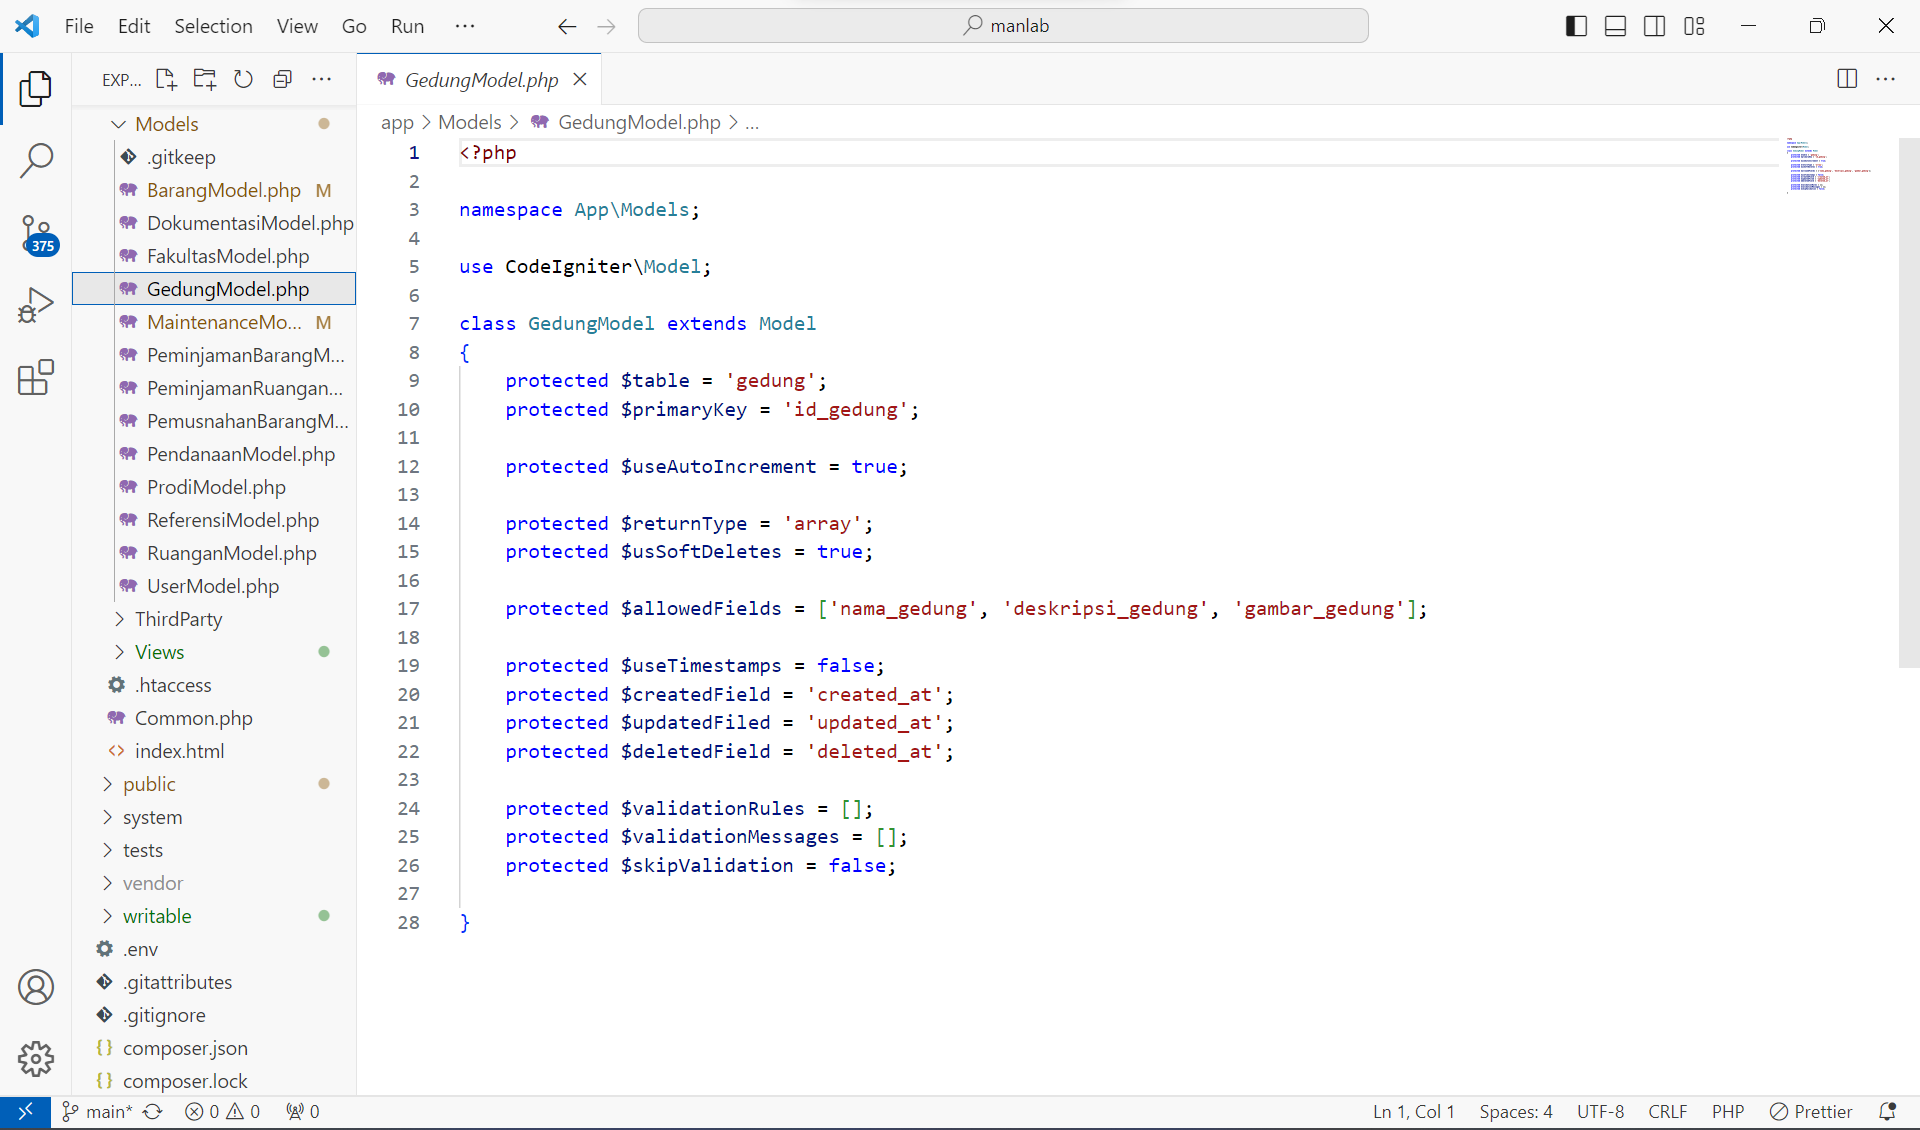
\includegraphics[width=0.82\linewidth]{konten//gambar/gedung model.png}
          \caption{Model Gedung}
          \label{fig:enter-label}
        \end{figure}

  \item Model dalam implementasi sistem informasi inventaris laboratorium pada data \textit{maintenance} dapat dilihat pada Gambar 4.31.

        \begin{figure}
          \centering
          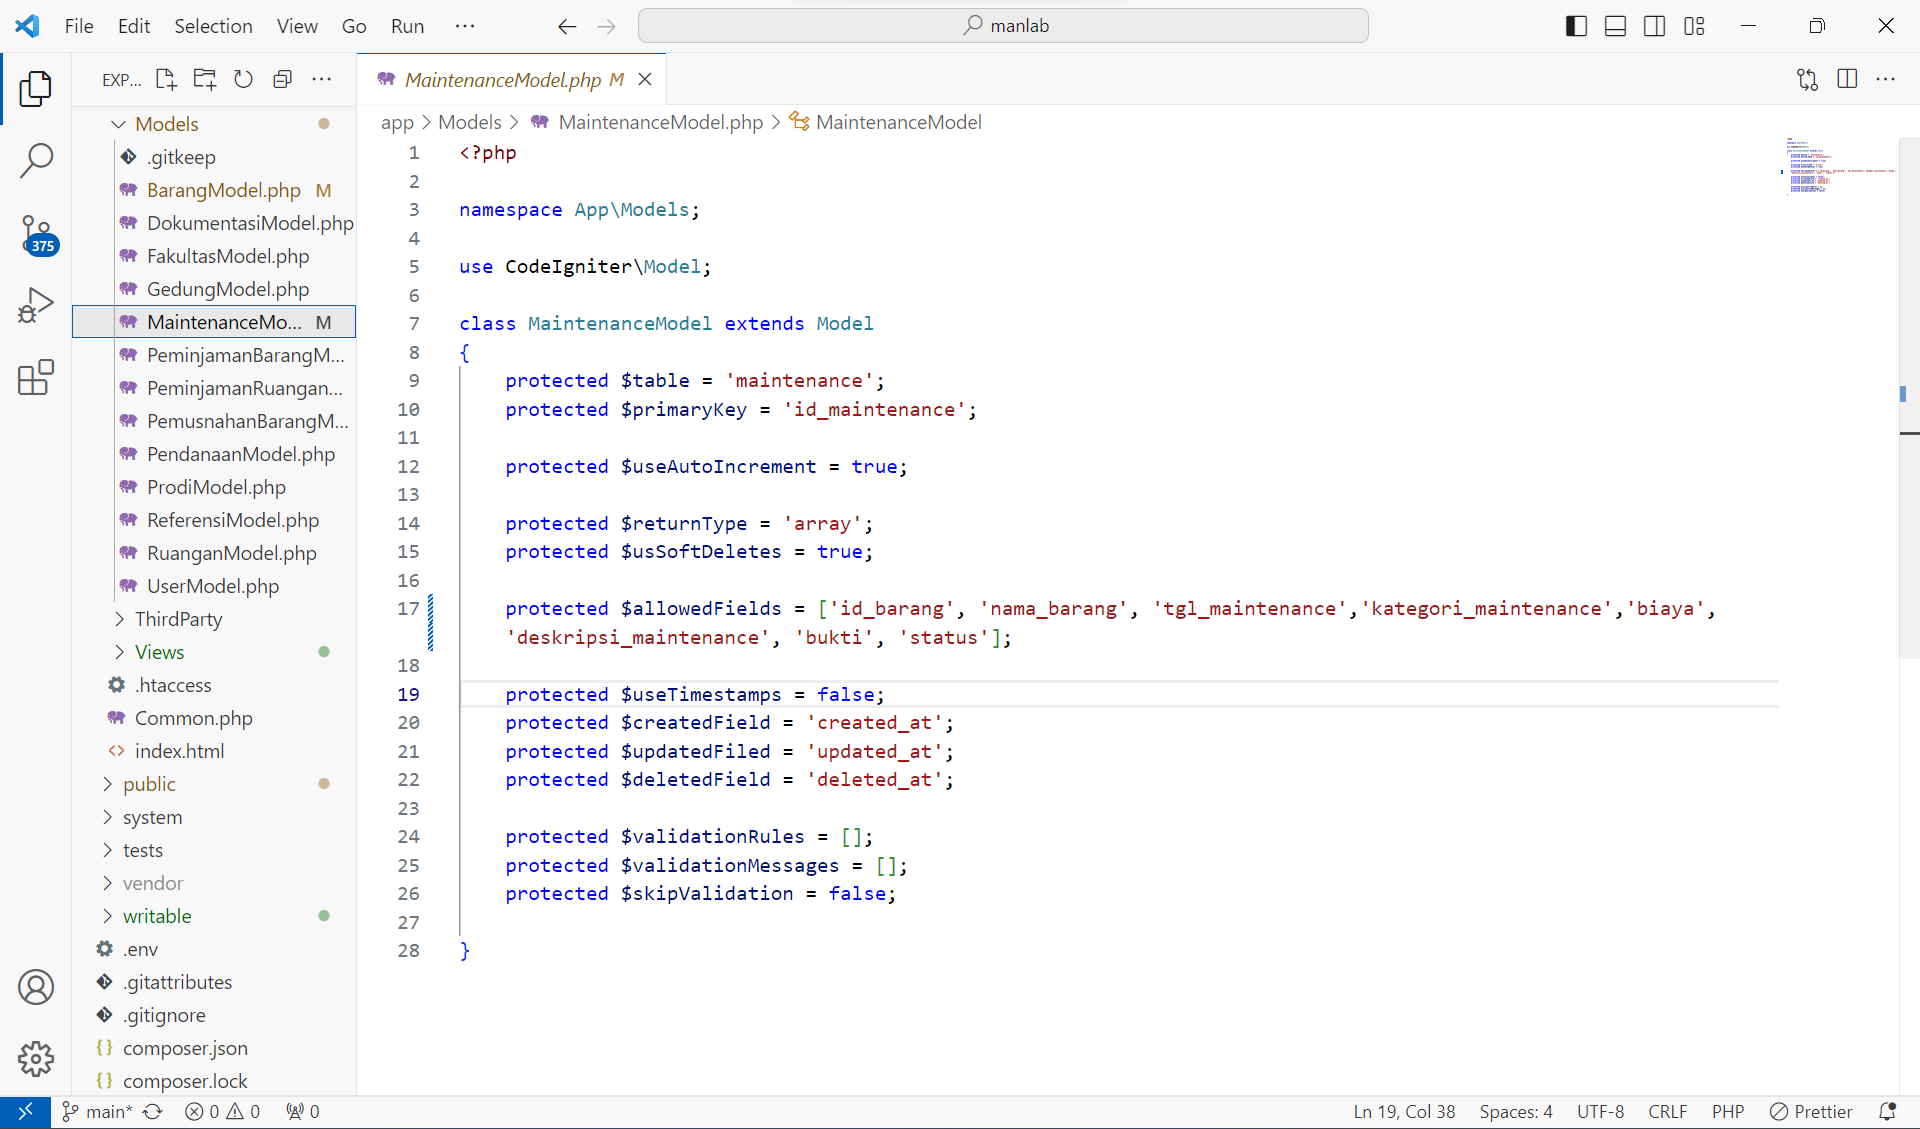
\includegraphics[width=0.82\linewidth]{konten//gambar/maintenance model.png}
          \caption{Model \textit{Maintenance}}
          \label{fig:enter-label}
        \end{figure}

  \item Model dalam implementasi sistem informasi inventaris laboratorium pada data peminjaman barang dapat dilihat pada Gambar 4.32.

        \begin{figure}
          \centering
          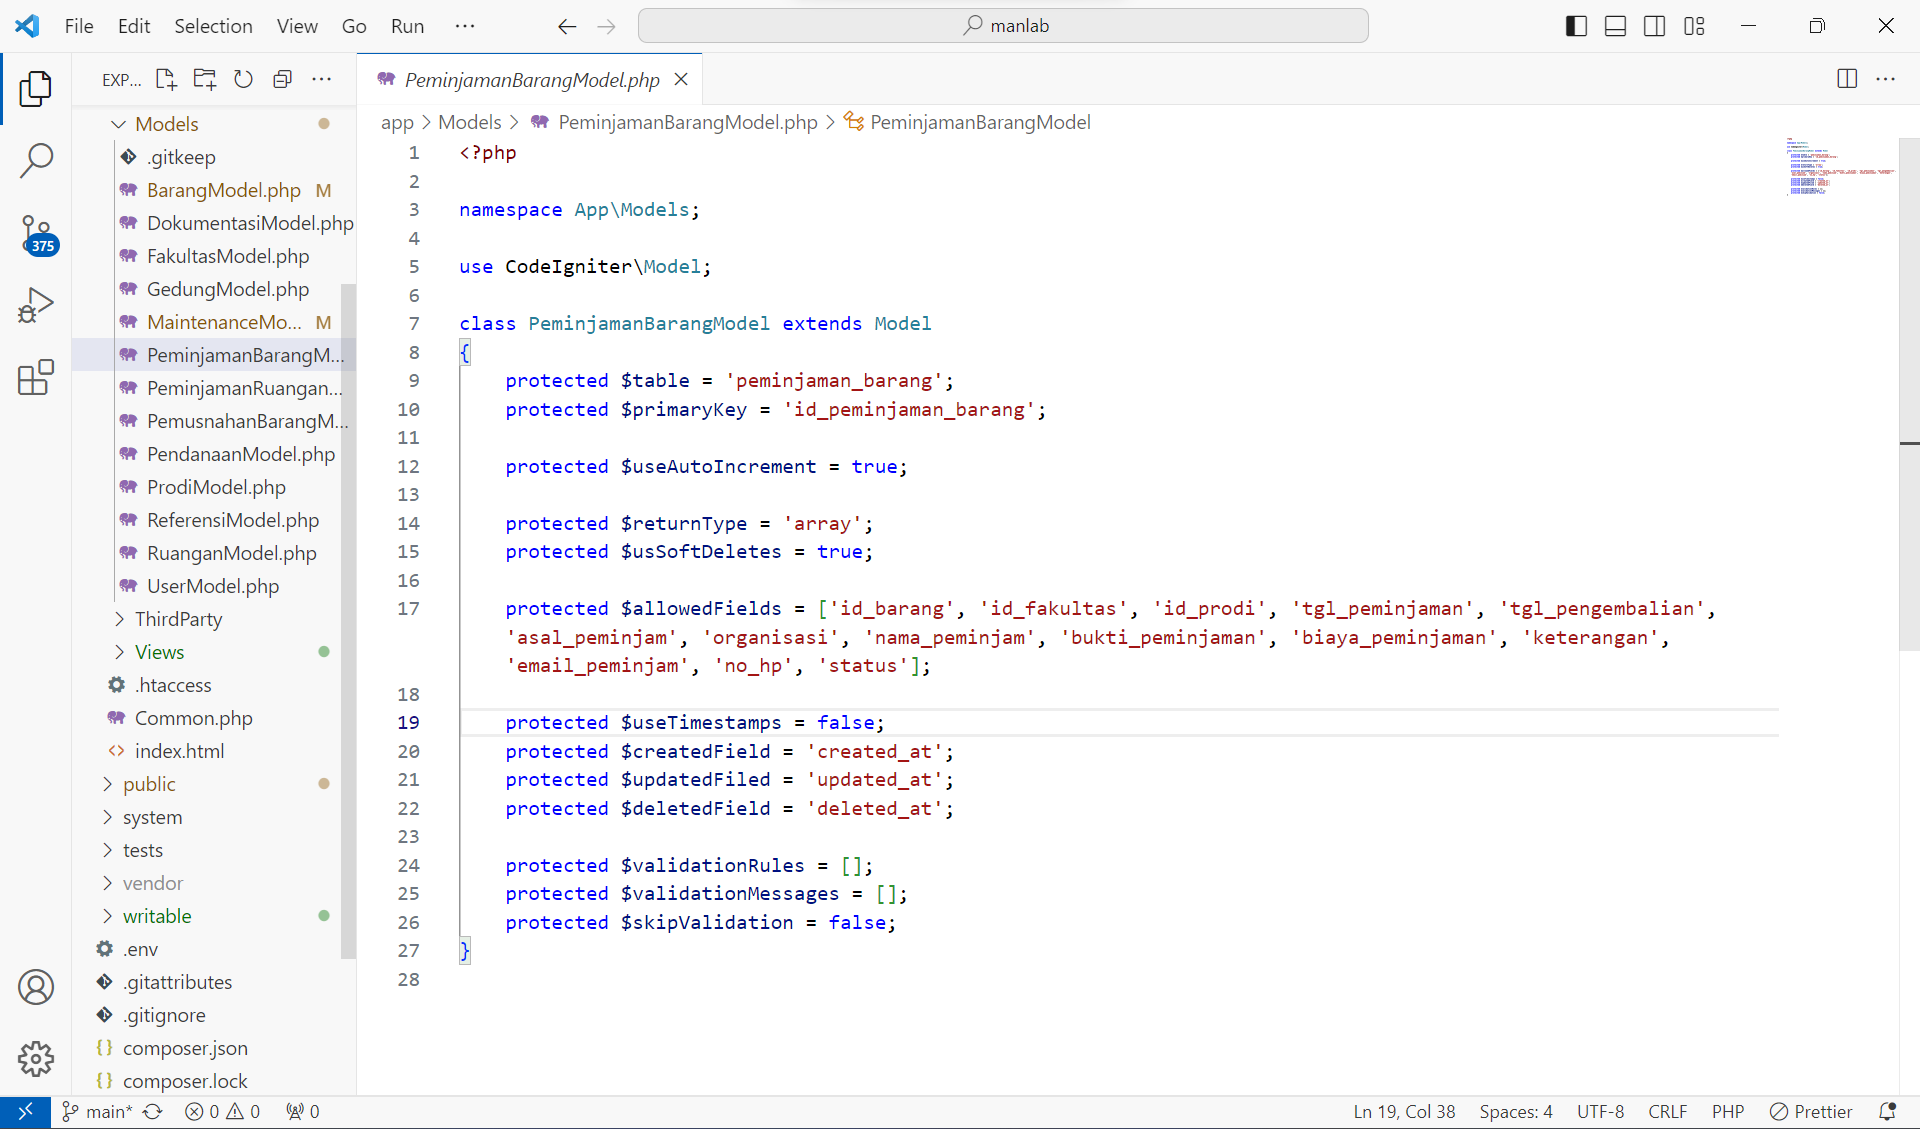
\includegraphics[width=0.82\linewidth]{konten//gambar/peminjaman barang model.png}
          \caption{Model Peminjaman Barang}
          \label{fig:enter-label}
        \end{figure}

  \item Model dalam implementasi sistem informasi inventaris laboratorium pada data peminjaman ruangan dapat dilihat pada Gambar 4.33.

        \begin{figure}
          \centering
          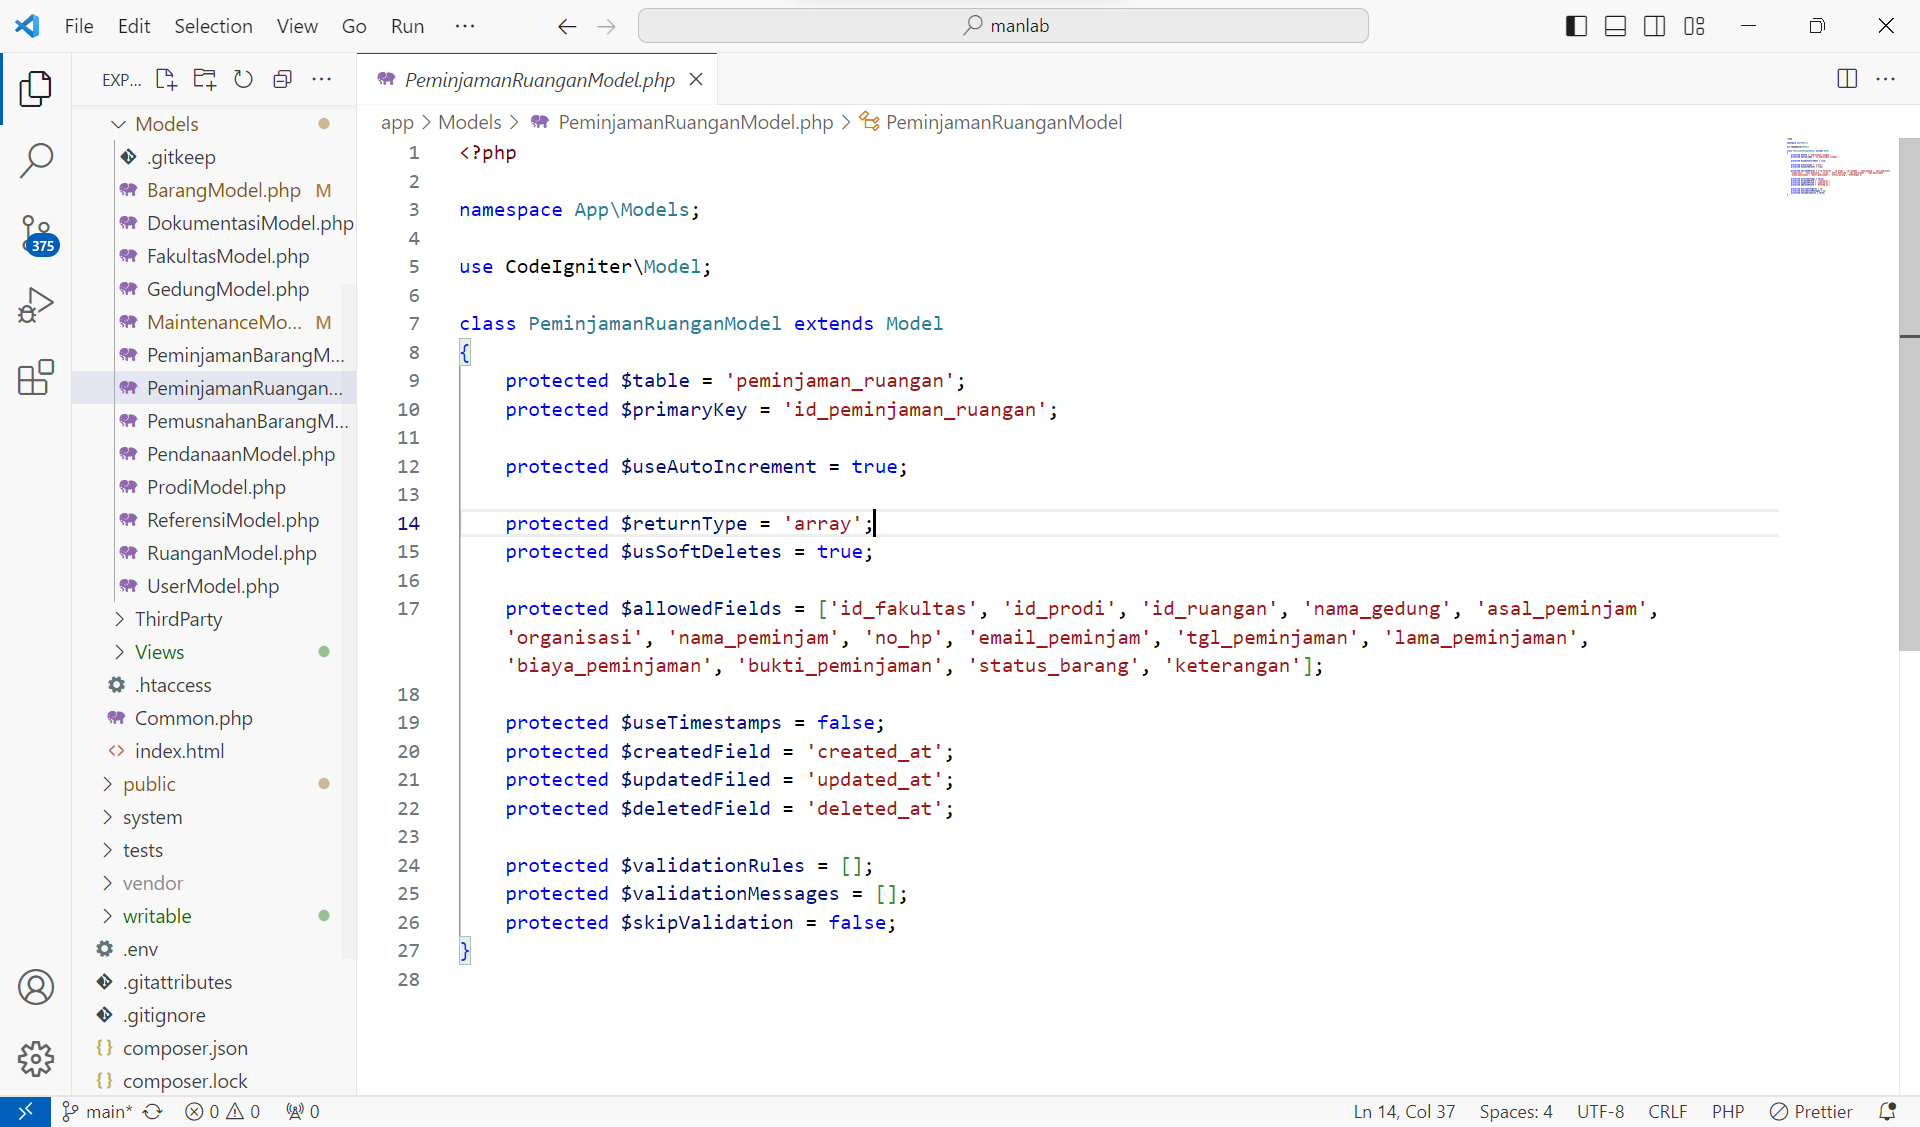
\includegraphics[width=0.82\linewidth]{konten//gambar/peminjaman ruangan model.png}
          \caption{Model Peminjaman Ruangan}
          \label{fig:enter-label}
        \end{figure}

  \item Model dalam implementasi sistem informasi inventaris laboratorium pada data pemusnahan barang dapat dilihat pada Gambar 4.34.

        \begin{figure}
          \centering
          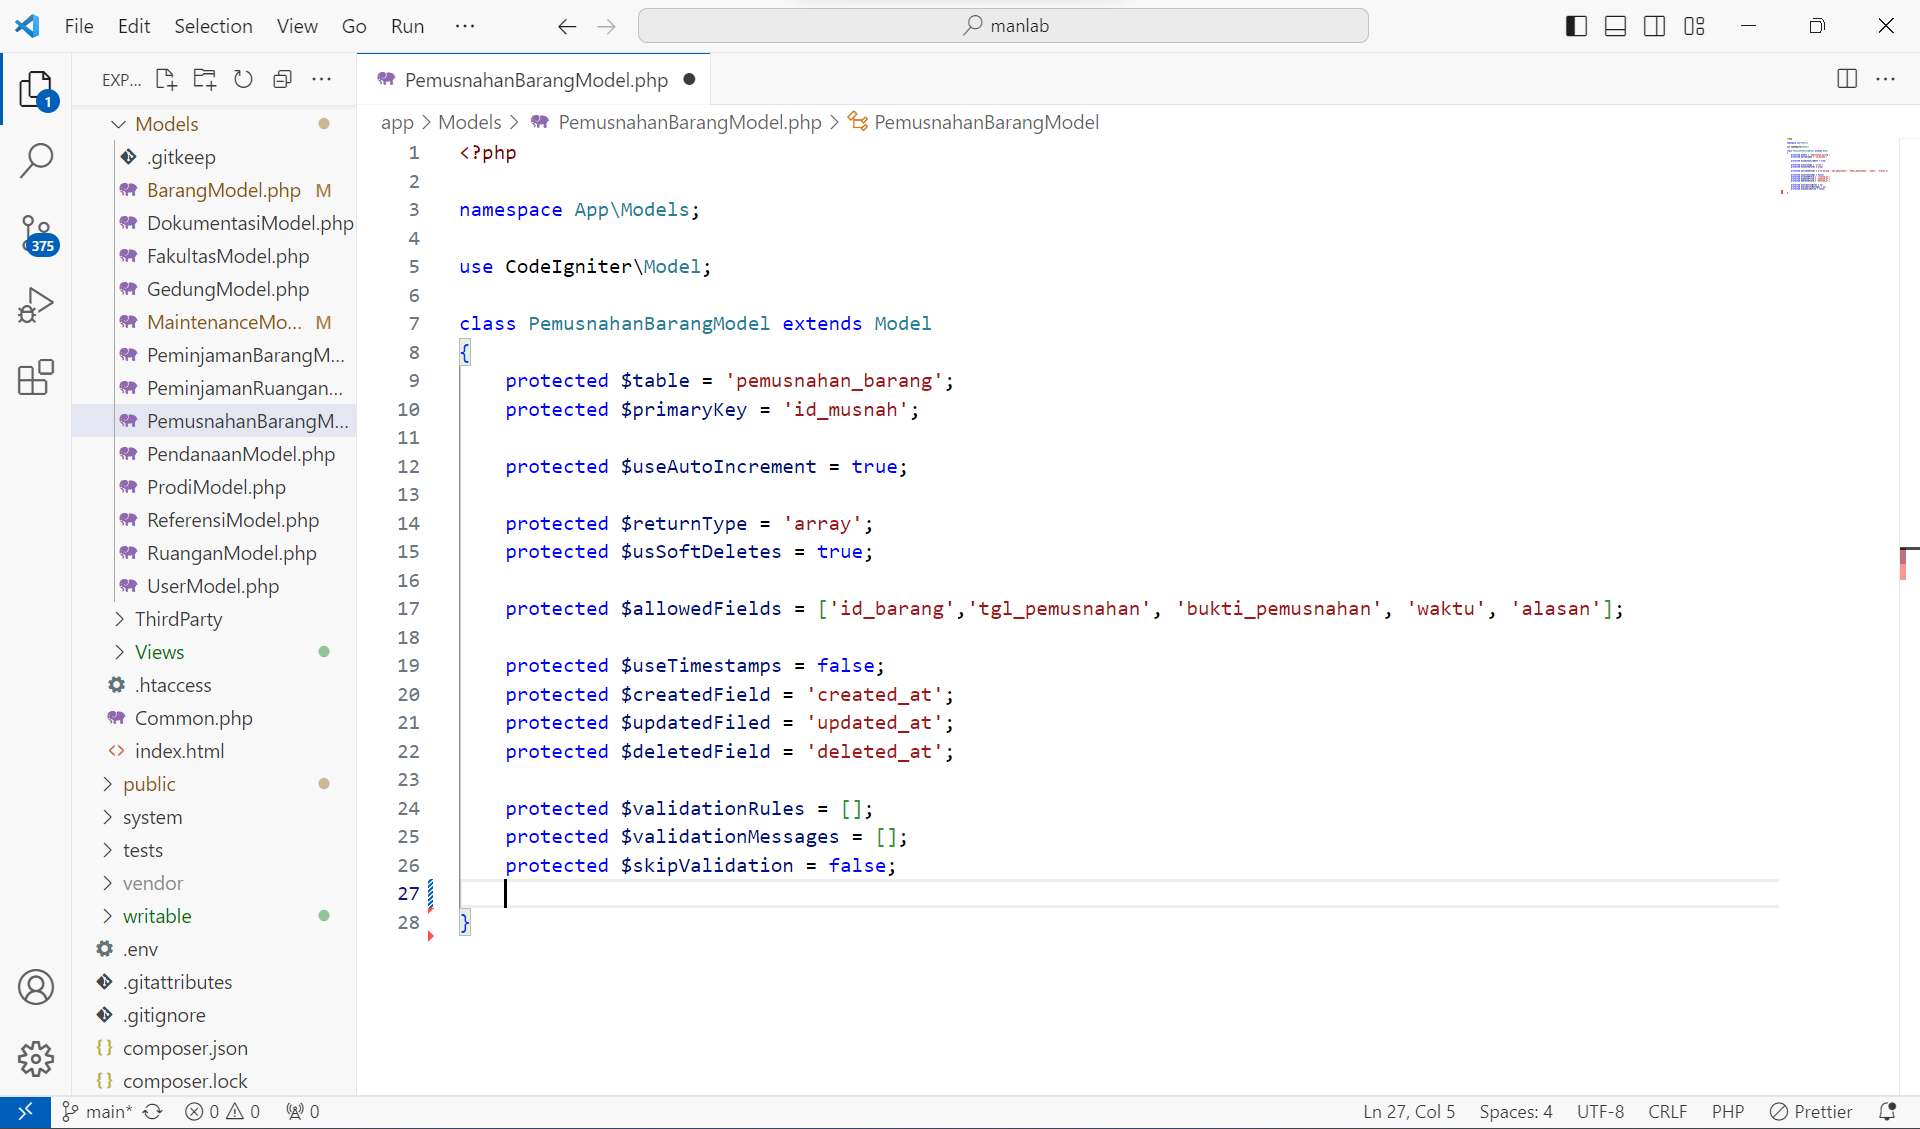
\includegraphics[width=0.82\linewidth]{konten//gambar/pemusnahan barang model.png}
          \caption{Model Pemusnahan Barang}
          \label{fig:enter-label}
        \end{figure}

  \item Model dalam implementasi sistem informasi inventaris laboratorium pada data pendanaan dapat dilihat pada Gambar 4.35.

        \begin{figure}
          \centering
          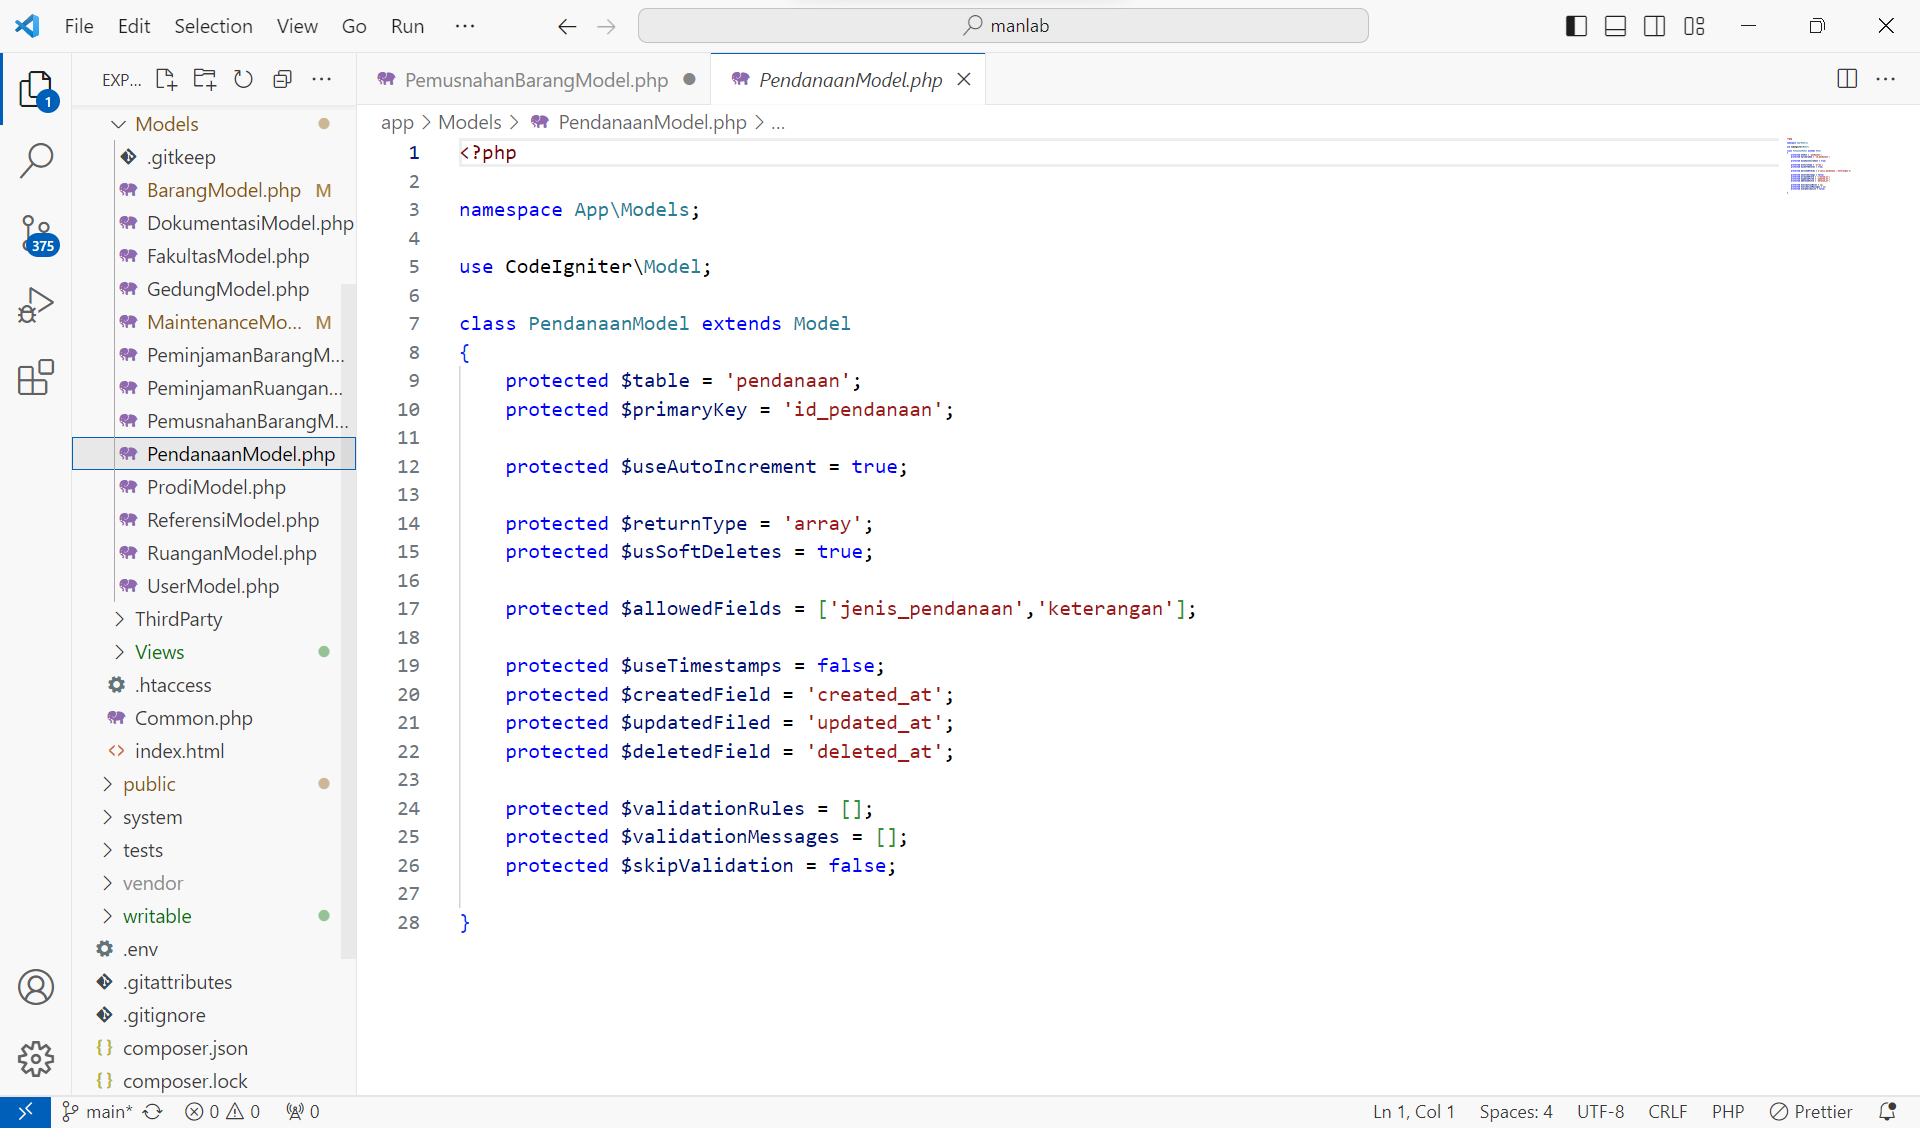
\includegraphics[width=0.82\linewidth]{konten//gambar/pendanaan model.png}
          \caption{Model Pendanaan}
          \label{fig:enter-label}
        \end{figure}

  \item Model dalam implementasi sistem informasi inventaris laboratorium pada data prodi dapat dilihat pada Gambar 4.36.

        \begin{figure}
          \centering
          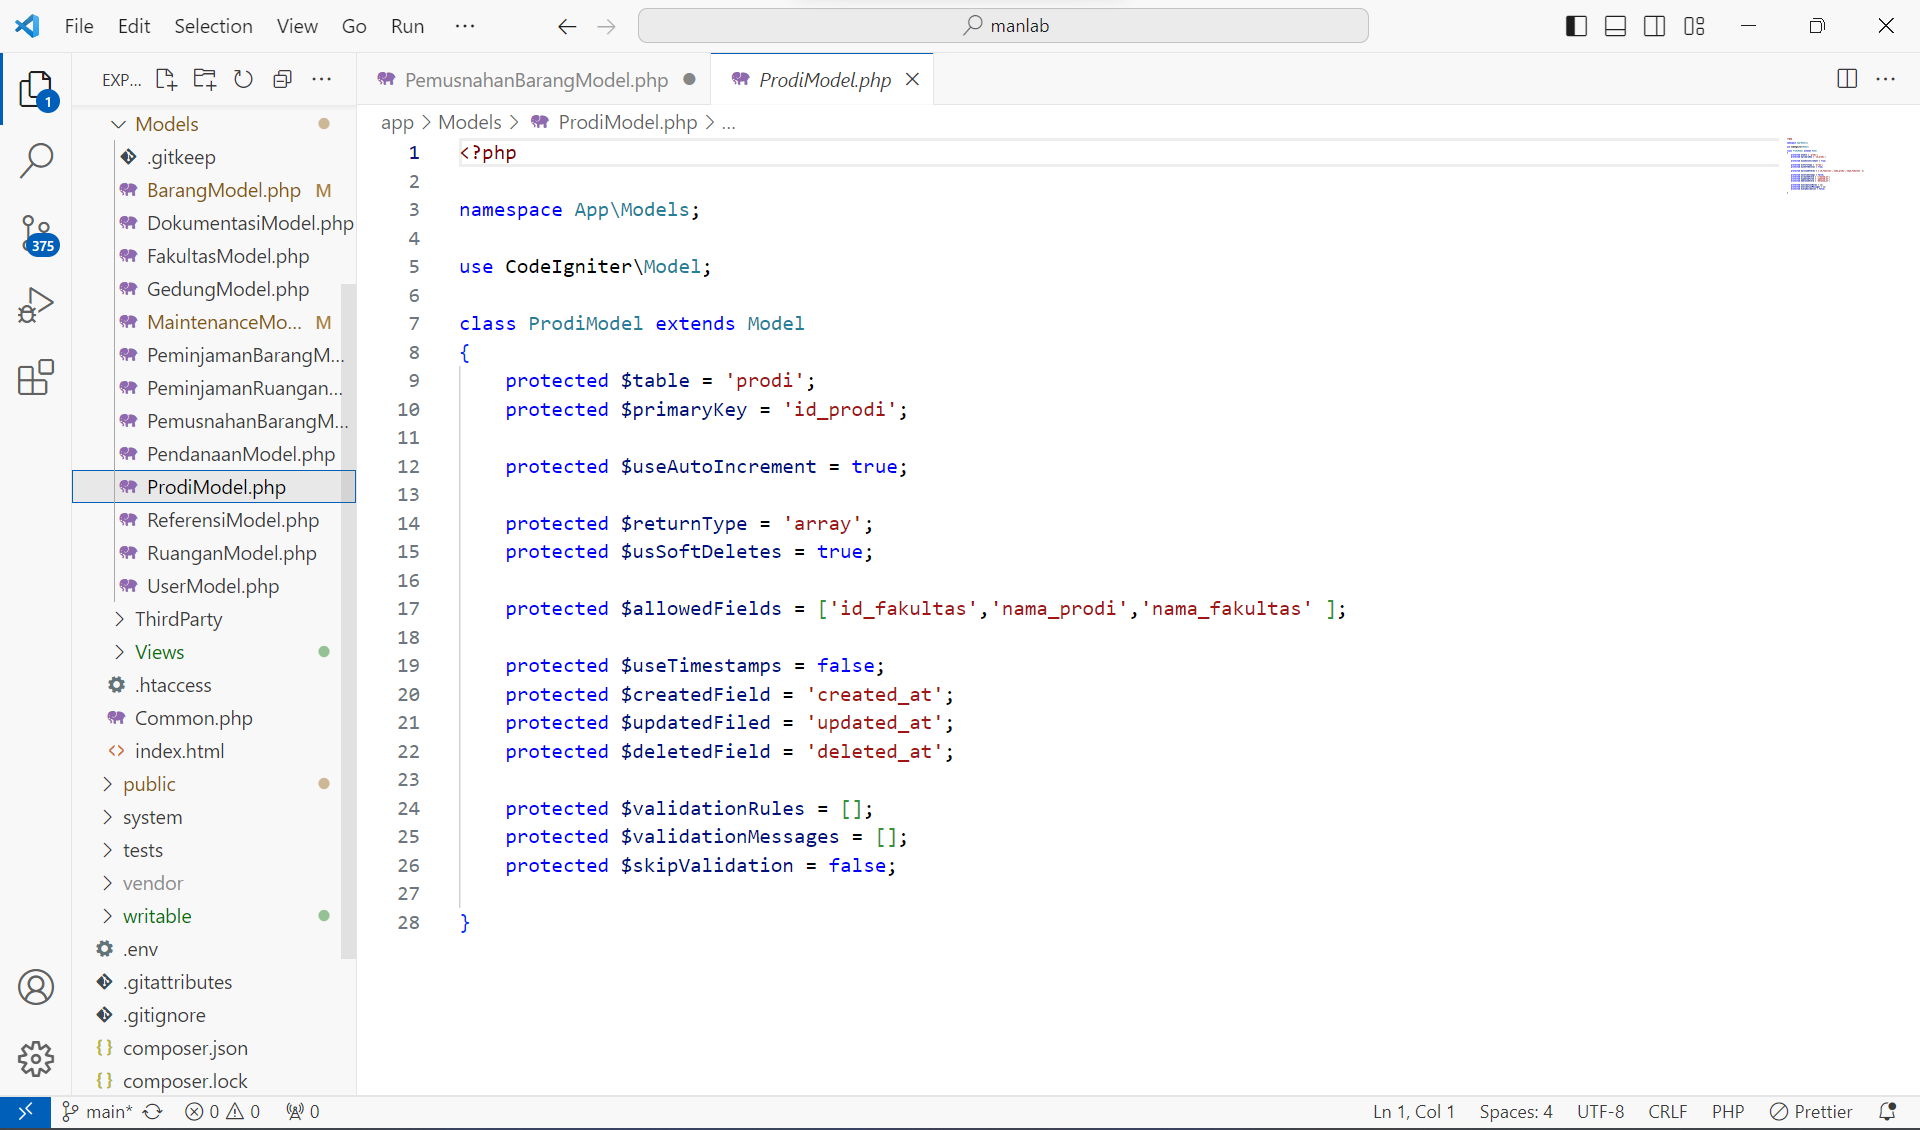
\includegraphics[width=0.82\linewidth]{konten//gambar/prodi model.png}
          \caption{Model Prodi}
          \label{fig:enter-label}
        \end{figure}

  \item Model dalam implementasi sistem informasi inventaris laboratorium pada data referensi dapat dilihat pada Gambar 4.37.

        \begin{figure}
          \centering
          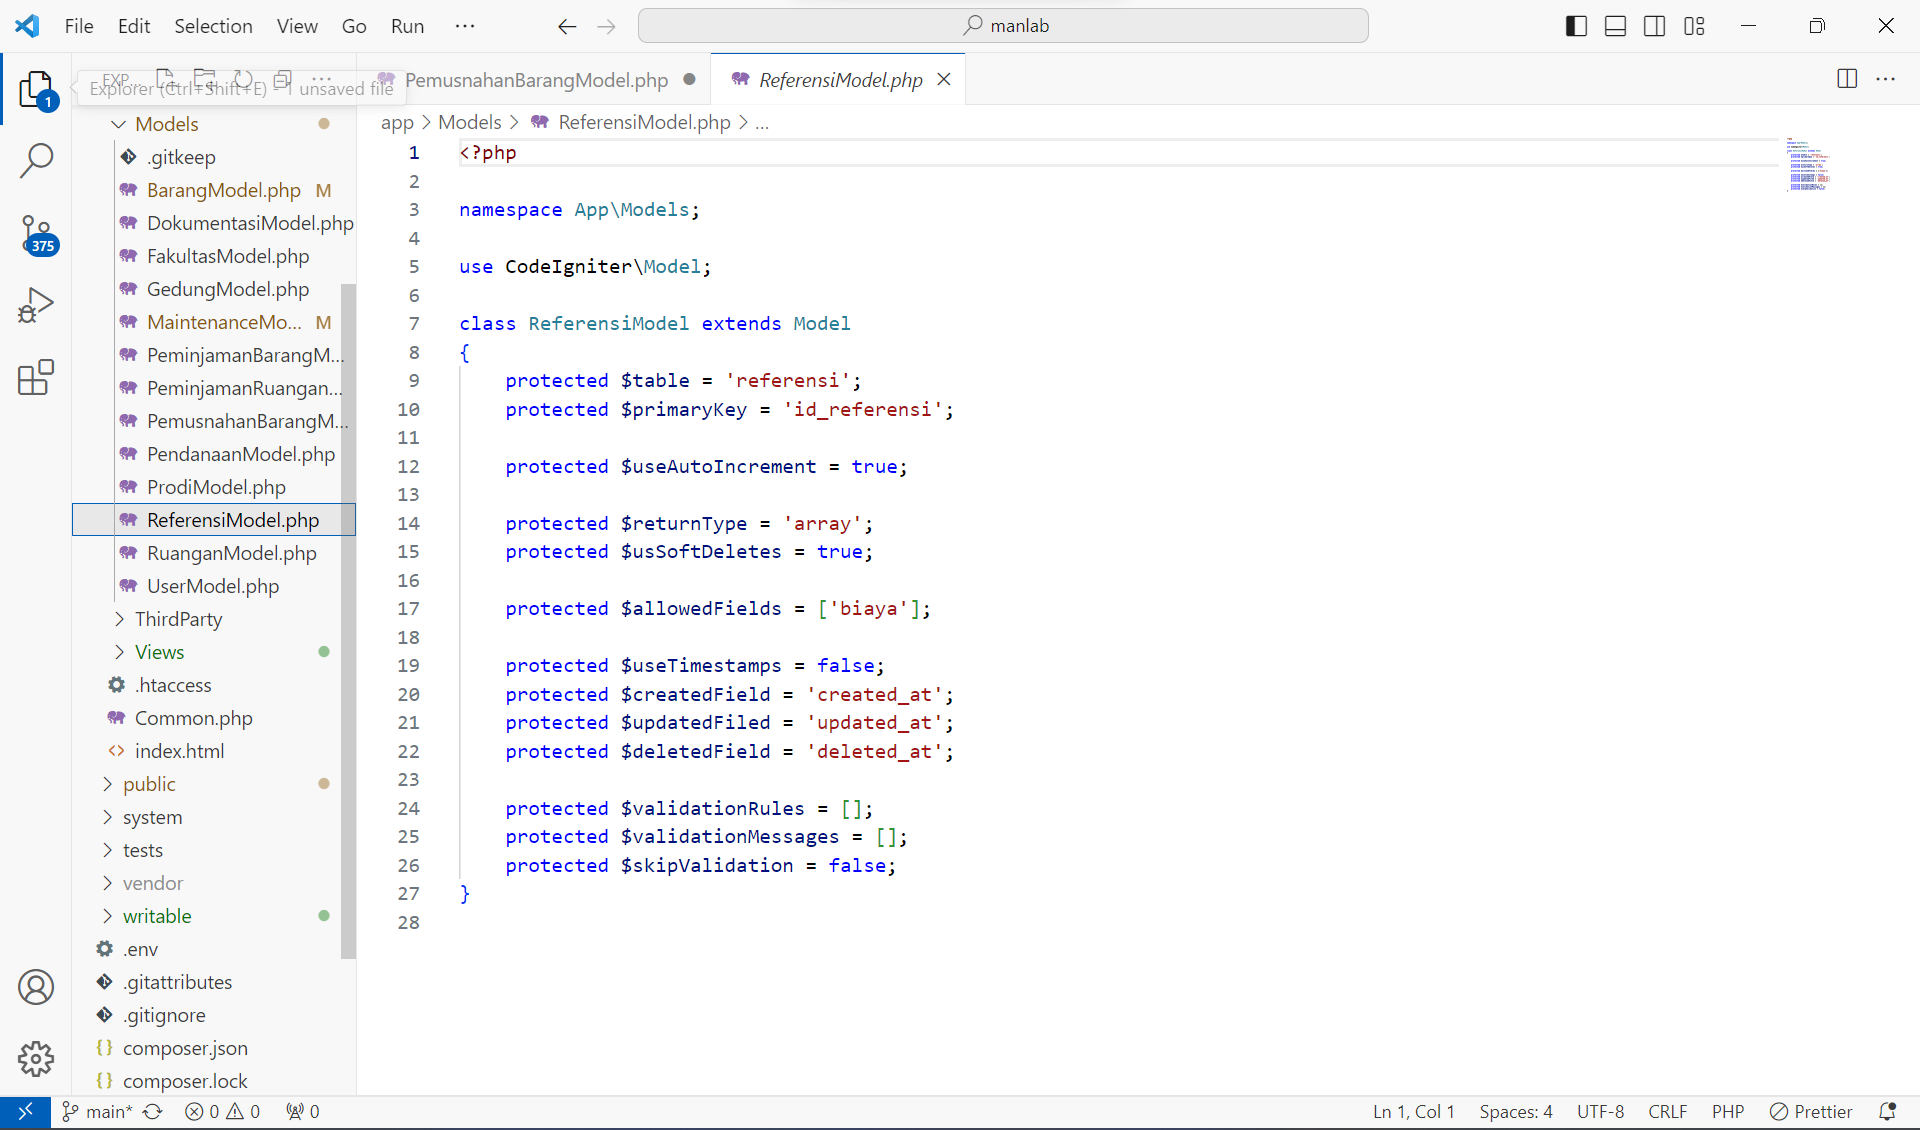
\includegraphics[width=0.82\linewidth]{konten//gambar/referensi model.png}
          \caption{Model Referensi}
          \label{fig:enter-label}
        \end{figure}

  \item Model dalam implementasi sistem informasi inventaris laboratorium pada data ruangan dapat dilihat pada Gambar 4.38.

        \begin{figure}
          \centering
          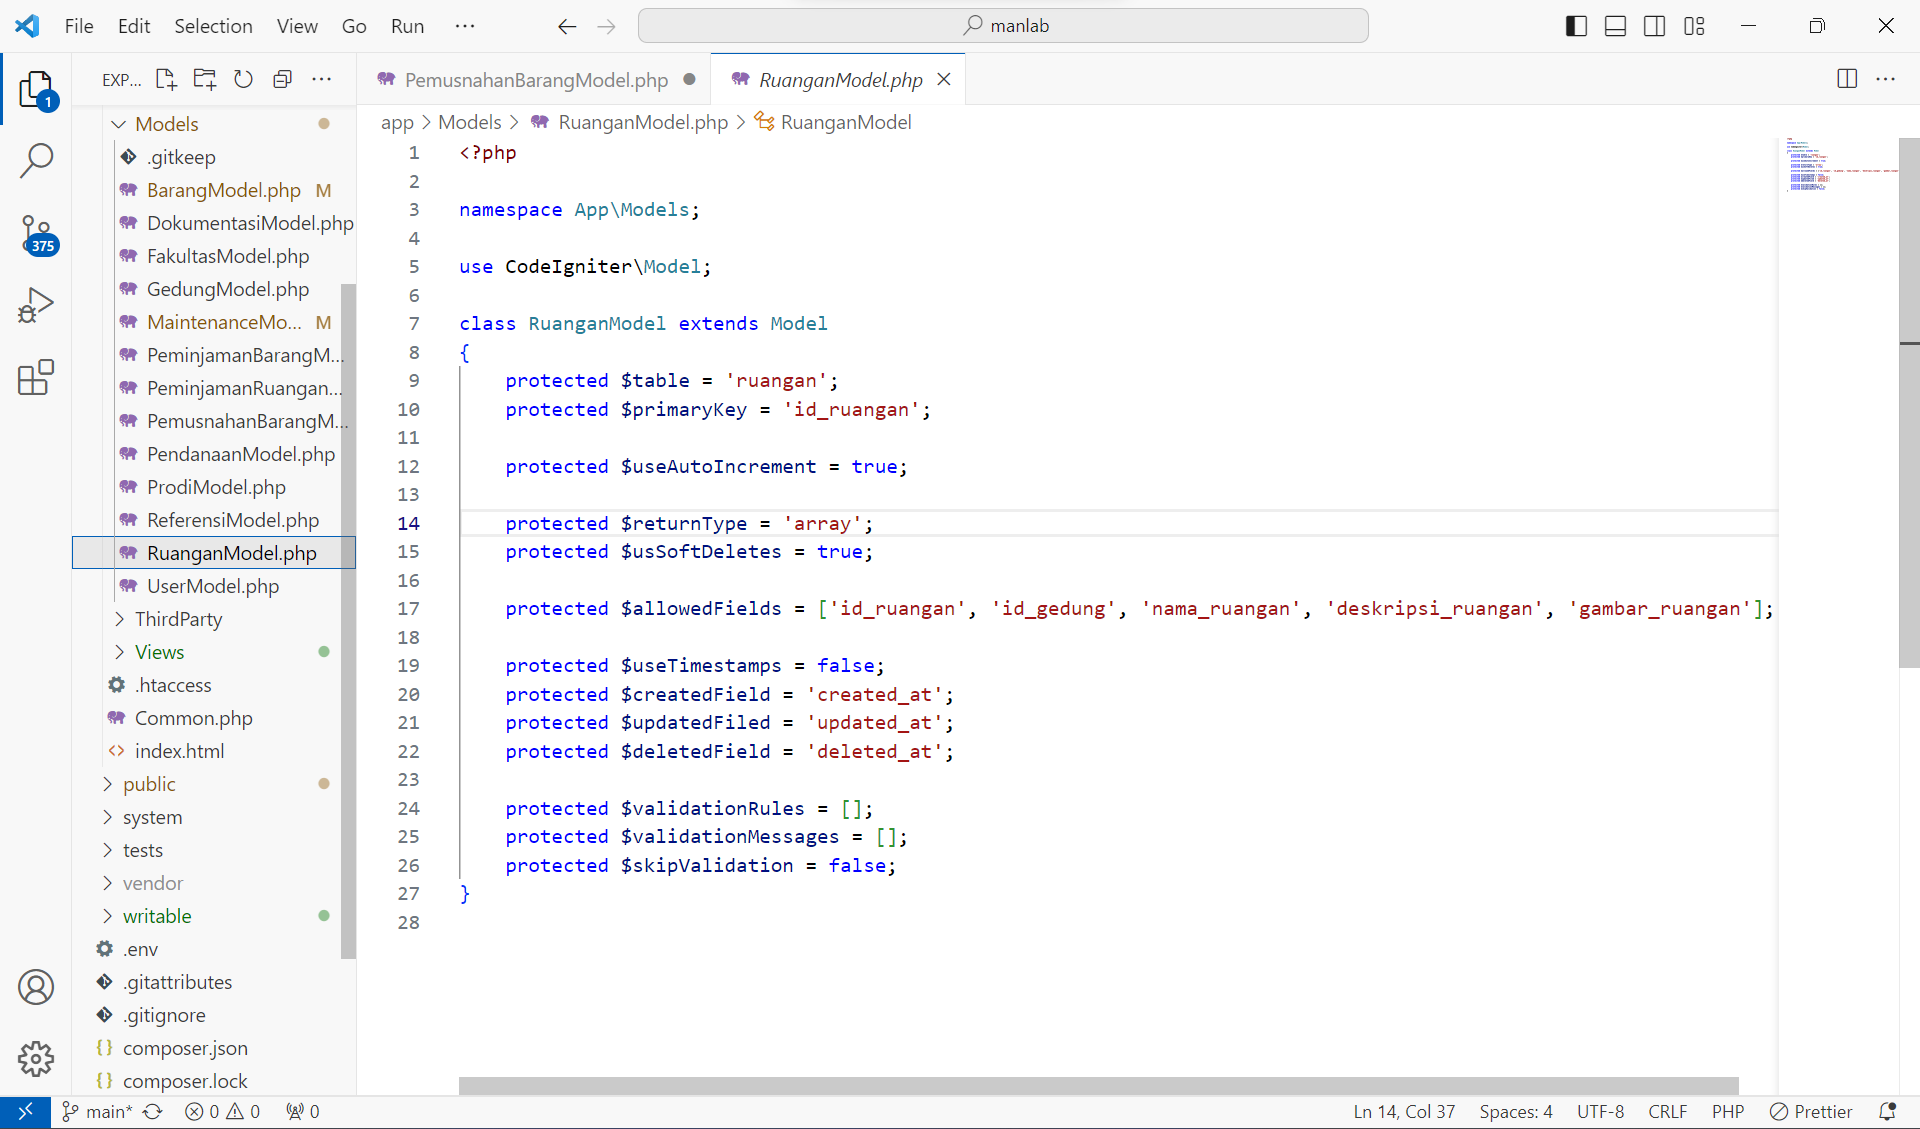
\includegraphics[width=0.82\linewidth]{konten//gambar/ruangan model.png}
          \caption{Model Ruangan}
          \label{fig:enter-label}
        \end{figure}

  \item Model dalam implementasi sistem informasi inventaris laboratorium pada data \textit{user} dapat dilihat pada Gambar 4.39.

        \begin{figure}
          \centering
          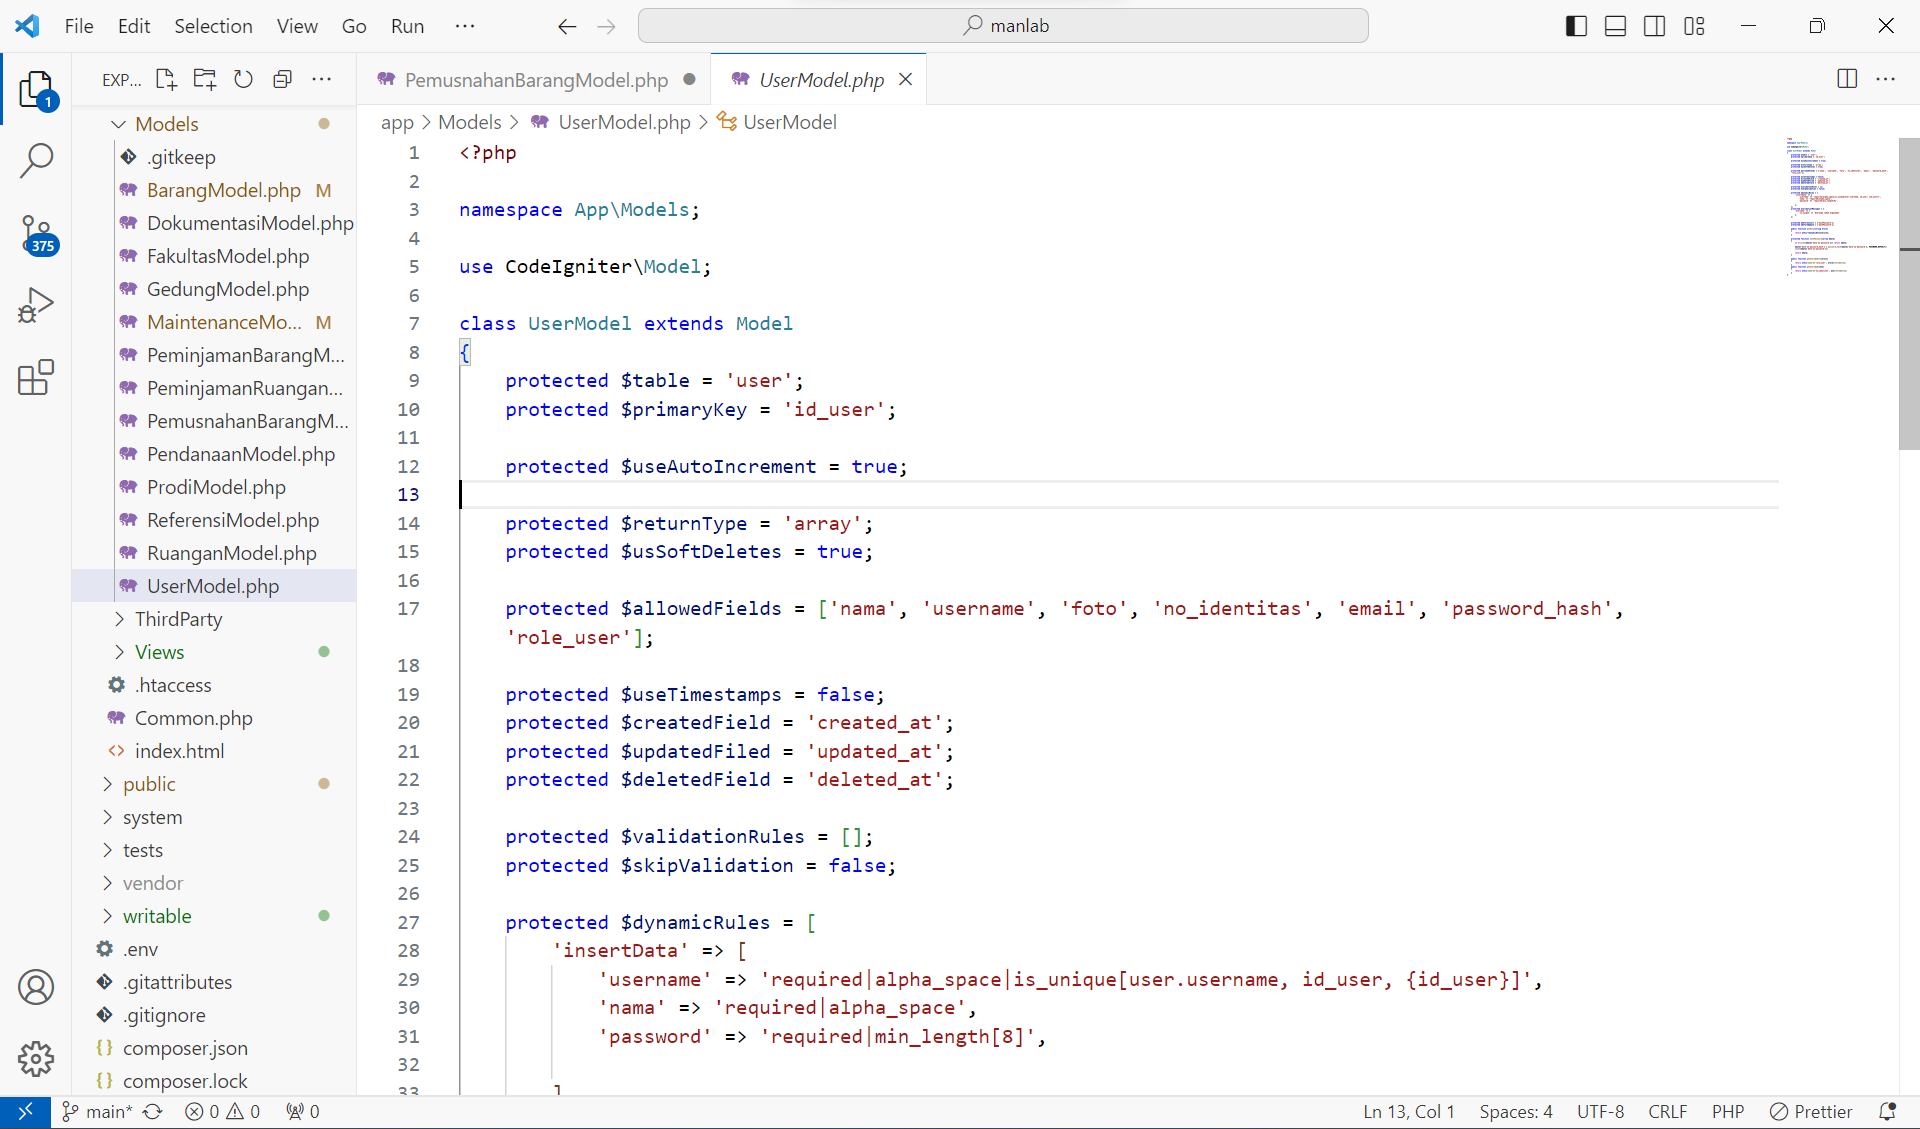
\includegraphics[width=0.82\linewidth]{konten//gambar/user model.png}
          \caption{Model \textit{User}}
          \label{fig:enter-label}
        \end{figure}

\end{enumerate}

\subsection{\textit{View}}
\textit{View }adalah komponen yang menampilkan antarmuka pengguna dan menampilkan data dari Model. \textit{View} mengamati perubahan pada Model dan \textit{Controller}, dan diperbarui sesuai keadaan terkini. Penggunaan \textit{View} memisahkan tugas penyajian dan manajemen data dalam aplikasi, yang memberikan fleksibilitas dan pemeliharaan yang lebih baik \cite{firdaus2020rancang}.

\begin{enumerate}
  \item \textit{View} dalam implementasi sistem informasi inventaris laboratorium pada data barang dapat dilihat pada Gambar 4.40.
        \begin{figure}
          \centering
          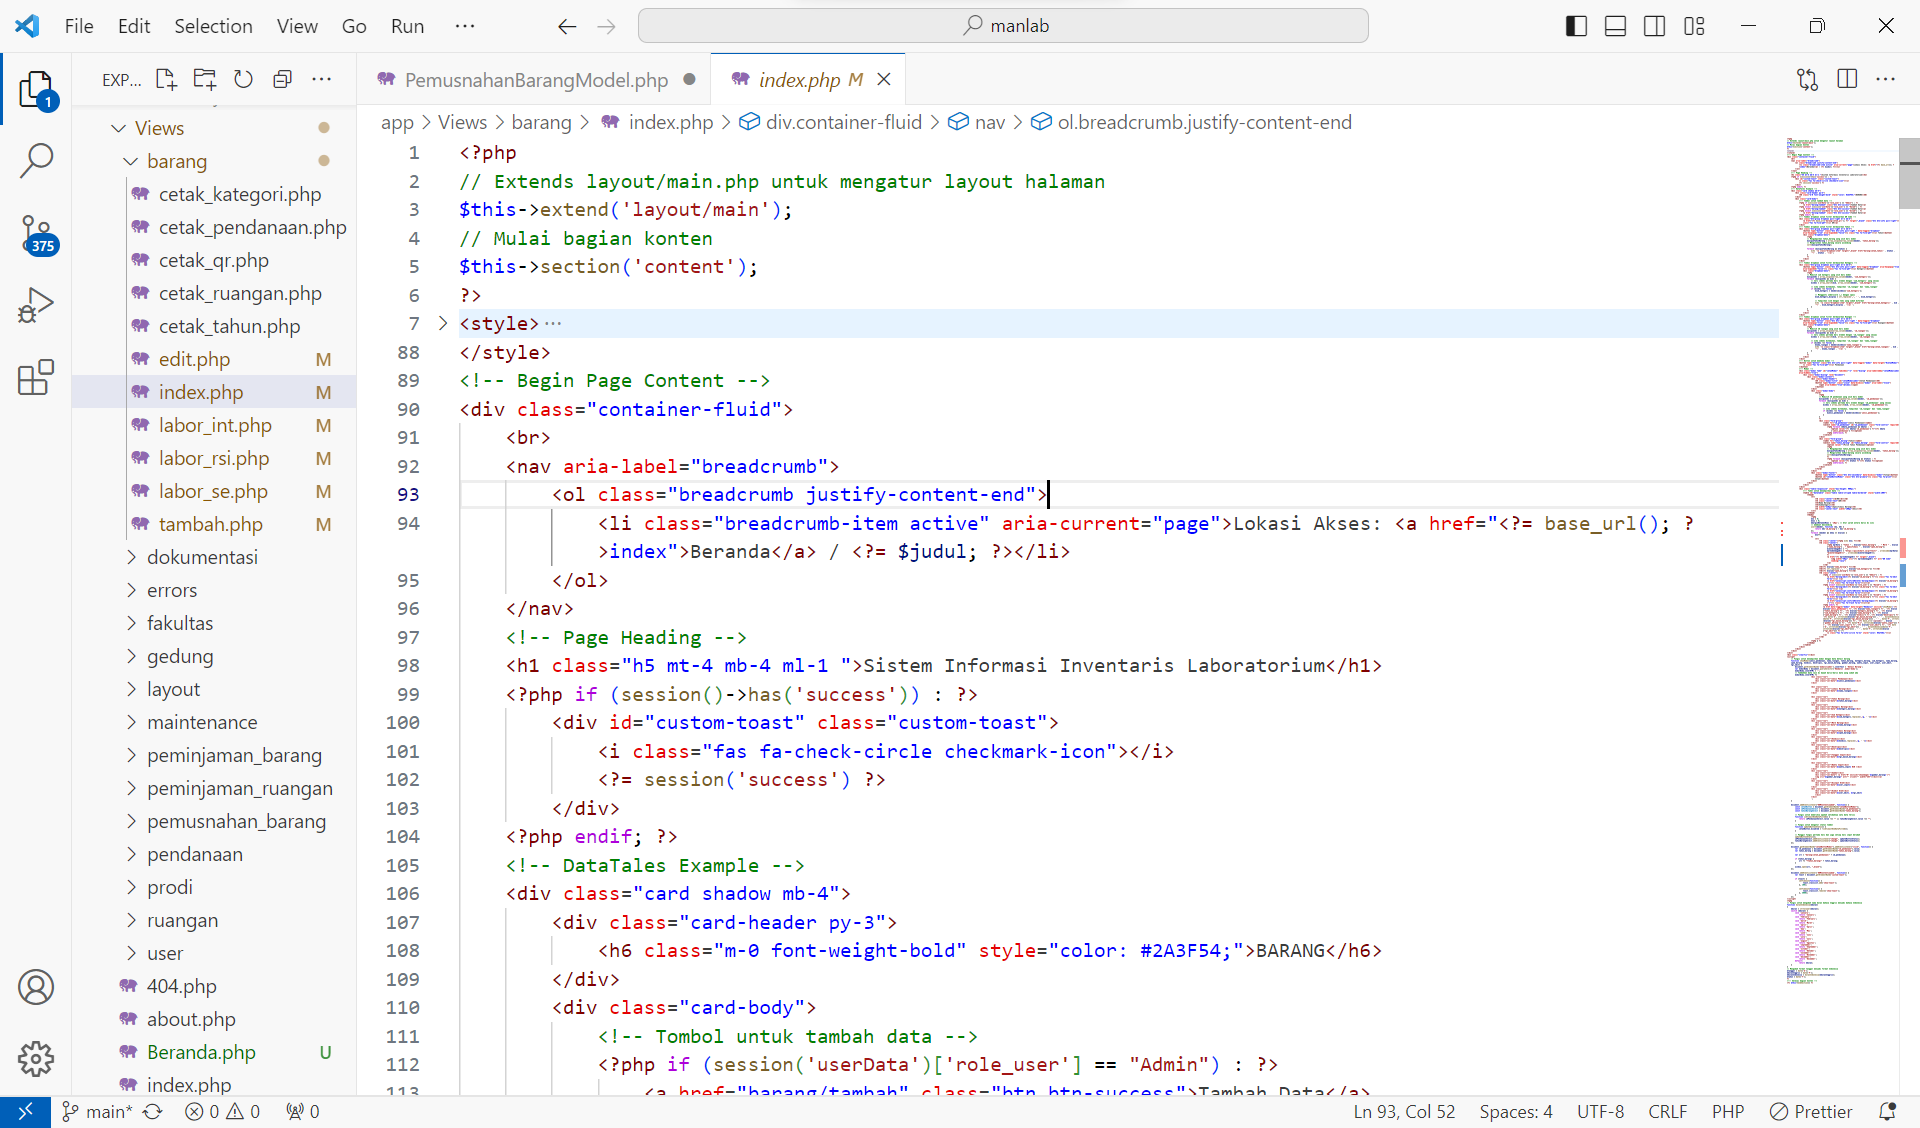
\includegraphics[width=0.82\linewidth]{konten//gambar/view barang.png}
          \caption{\textit{View} Barang}
          \label{fig:enter-label}
        \end{figure}

  \item \textit{View} dalam implementasi sistem informasi inventaris laboratorium pada data dokumentasi dapat dilihat pada Gambar 4.41.
        \begin{figure}
          \centering
          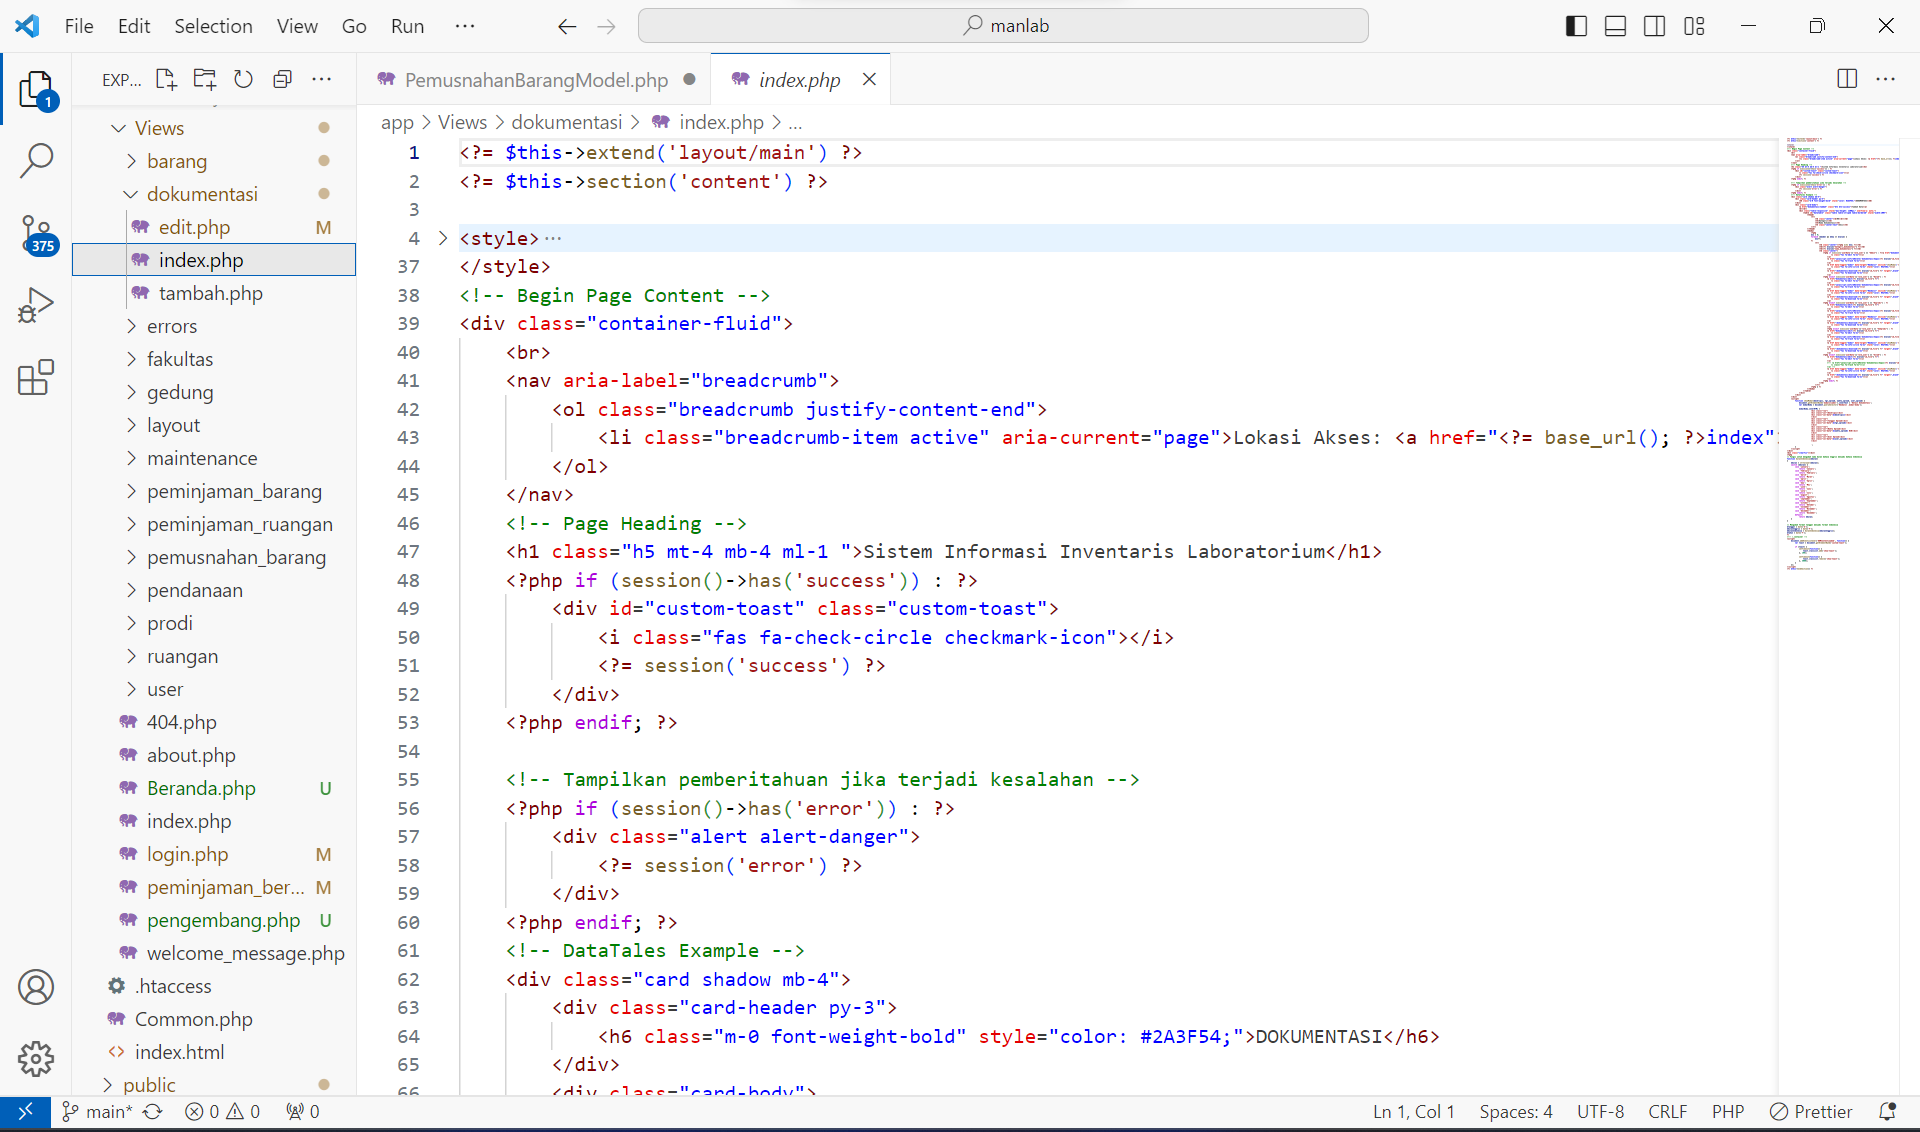
\includegraphics[width=0.82\linewidth]{konten//gambar/view dokumentasi.png}
          \caption{\textit{View} Dokumentasi}
          \label{fig:enter-label}
        \end{figure}

  \item \textit{View} dalam implementasi sistem informasi inventaris laboratorium pada data fakultas dapat dilihat pada Gambar 4.42.
        \begin{figure}
          \centering
          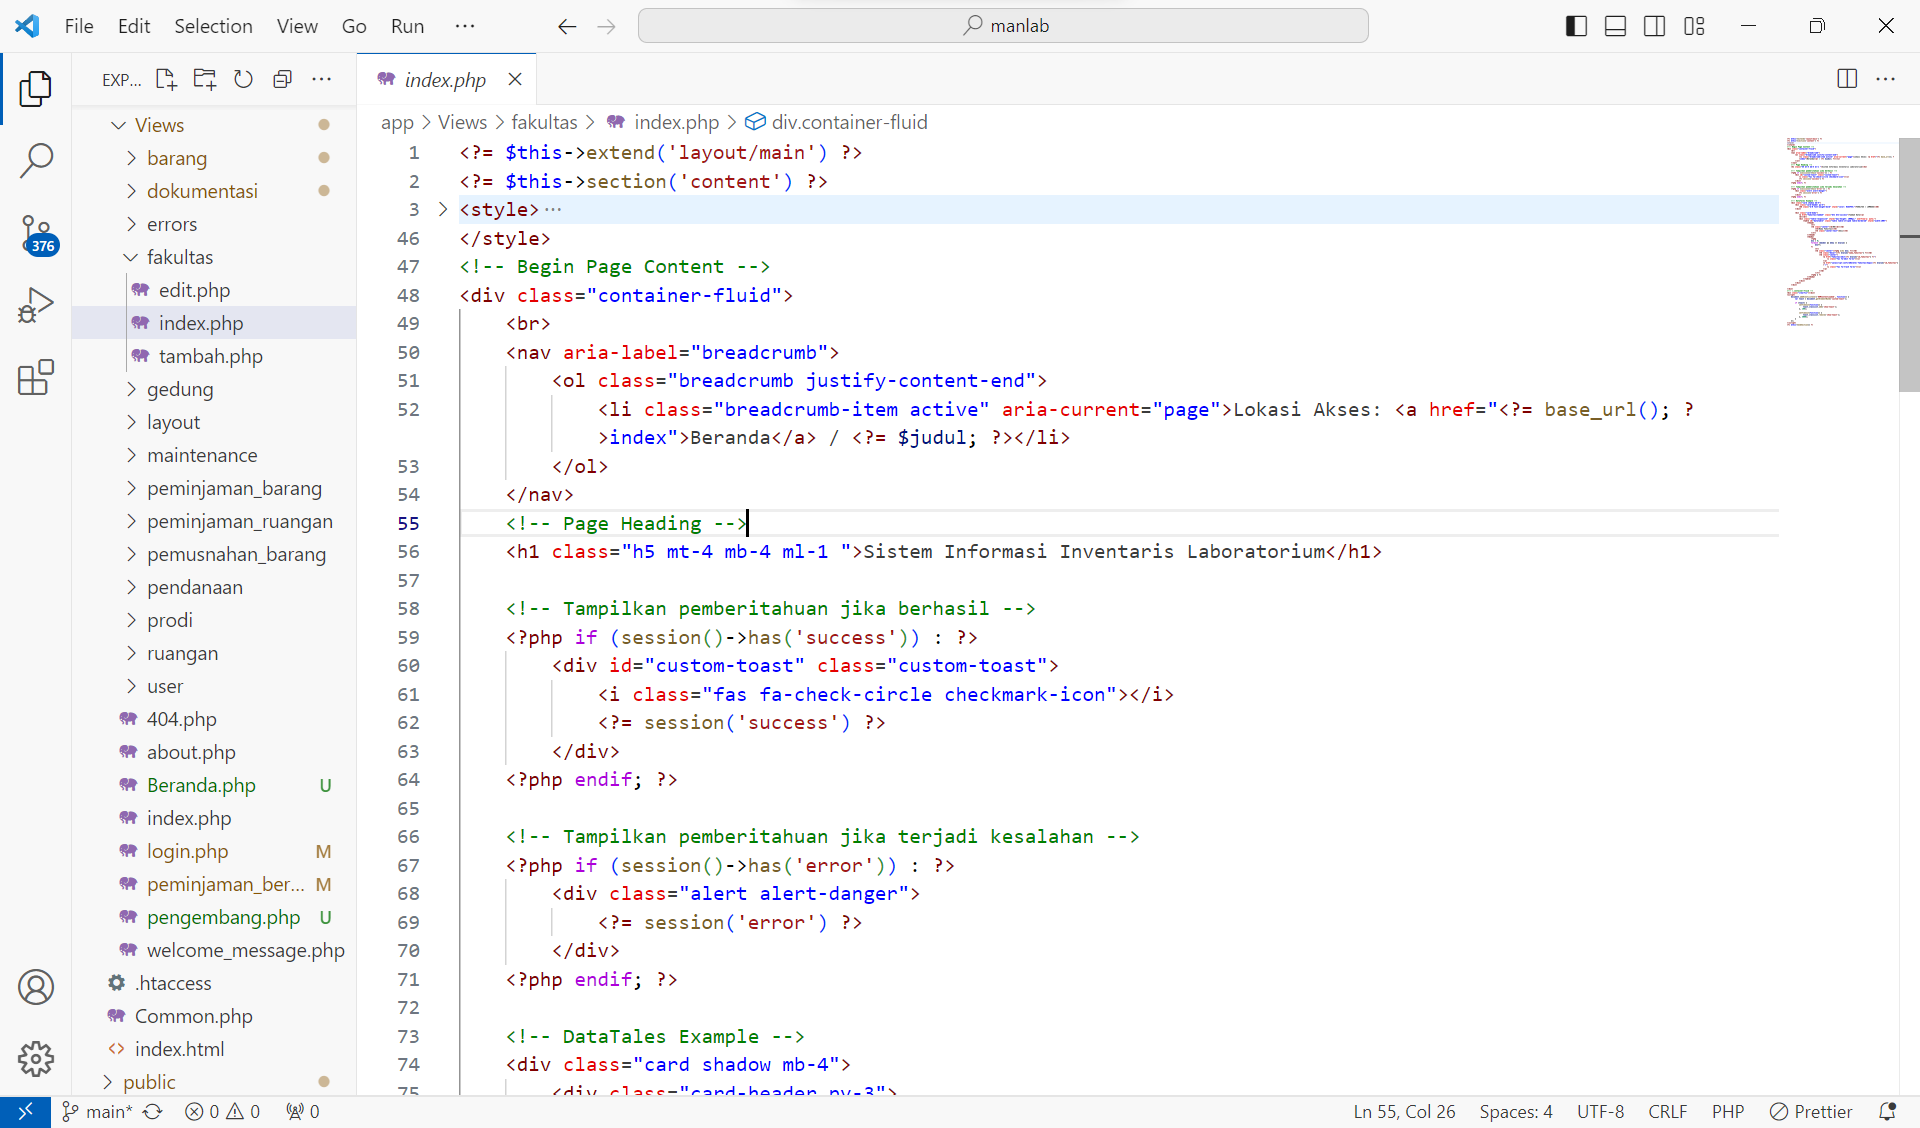
\includegraphics[width=0.82\linewidth]{konten//gambar/view fakultas.png}
          \caption{\textit{View} Fakultas}
          \label{fig:enter-label}
        \end{figure}

  \item \textit{View} dalam implementasi sistem informasi inventaris laboratorium pada data gedung dapat dilihat pada Gambar 4.43.
        \begin{figure}
          \centering
          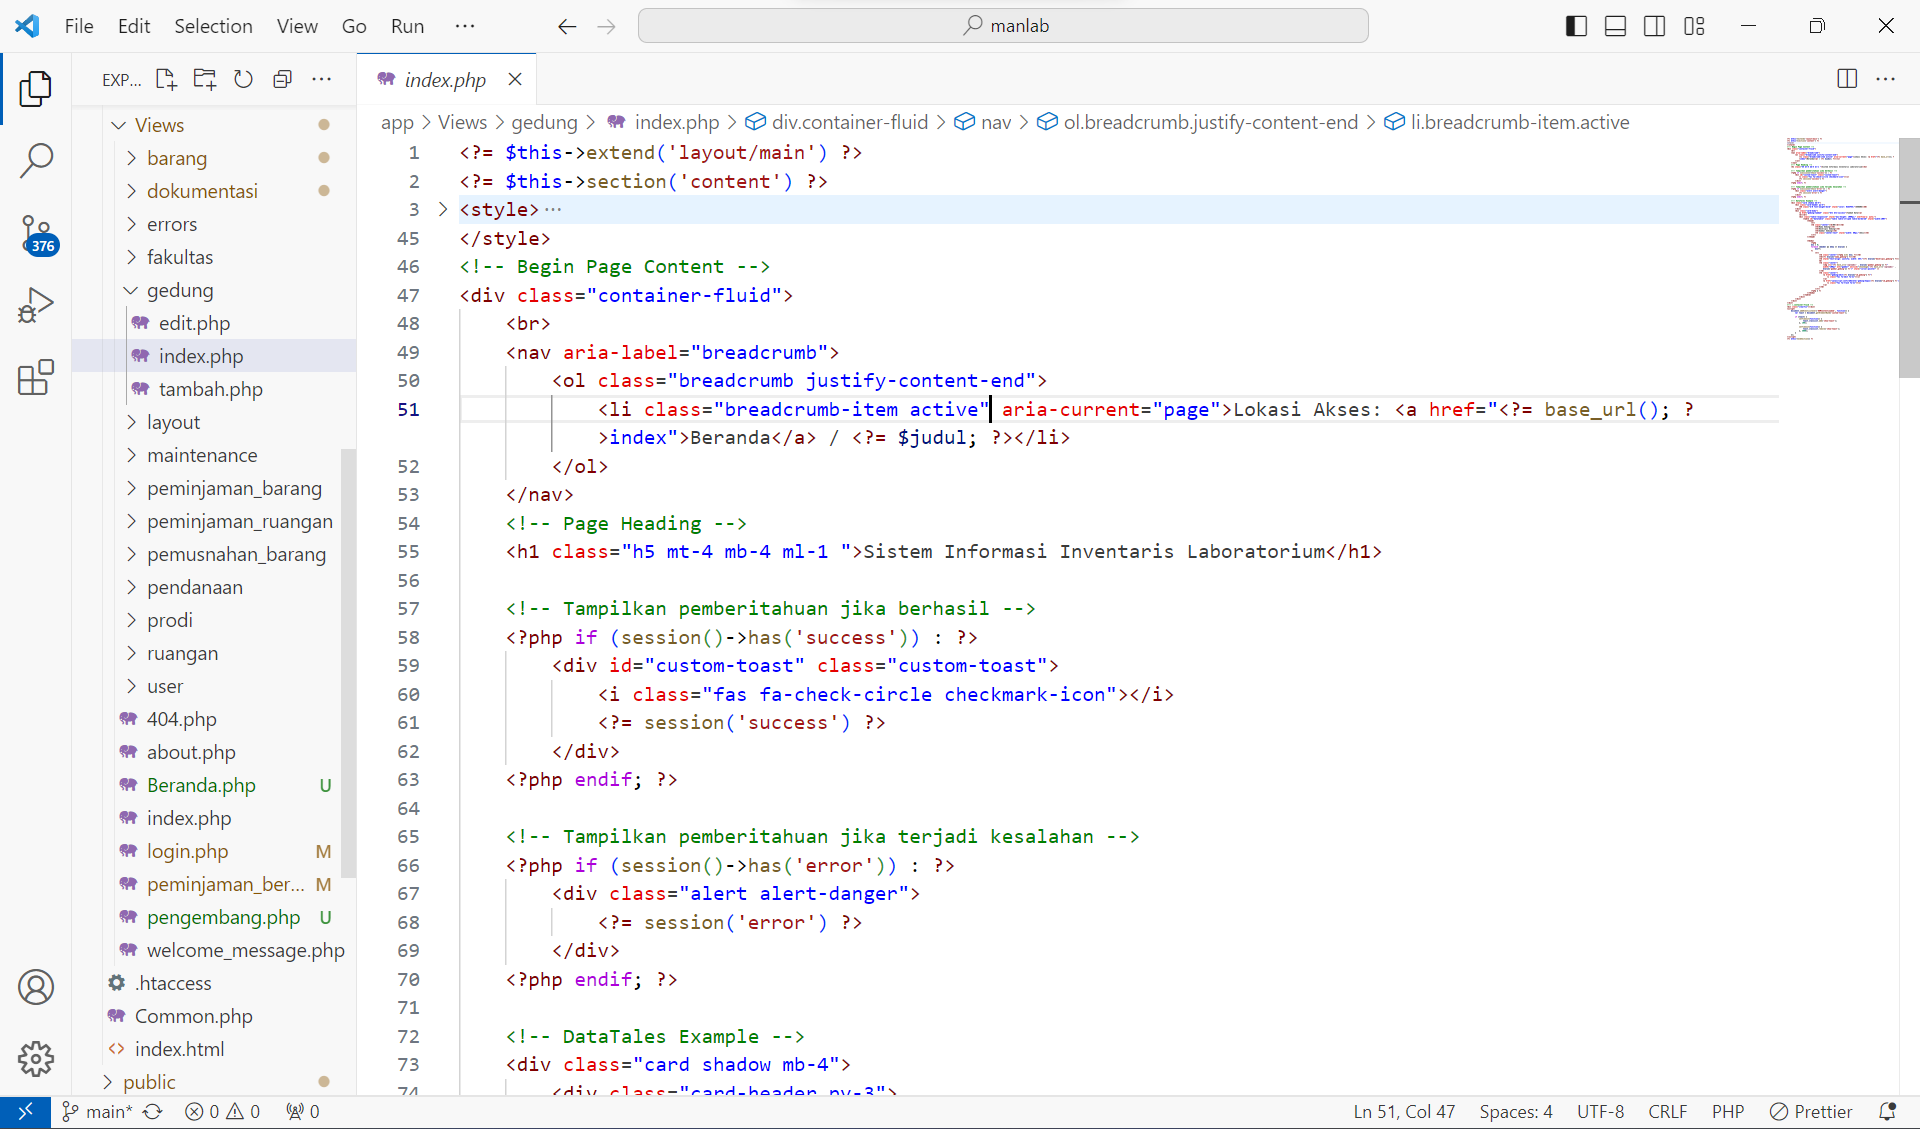
\includegraphics[width=0.82\linewidth]{konten//gambar/view gedung.png}
          \caption{\textit{View} Gedung}
          \label{fig:enter-label}
        \end{figure}

  \item \textit{View} dalam implementasi sistem informasi inventaris laboratorium pada data \textit{maintenance} dapat dilihat pada Gambar 4.44.
        \begin{figure}
          \centering
          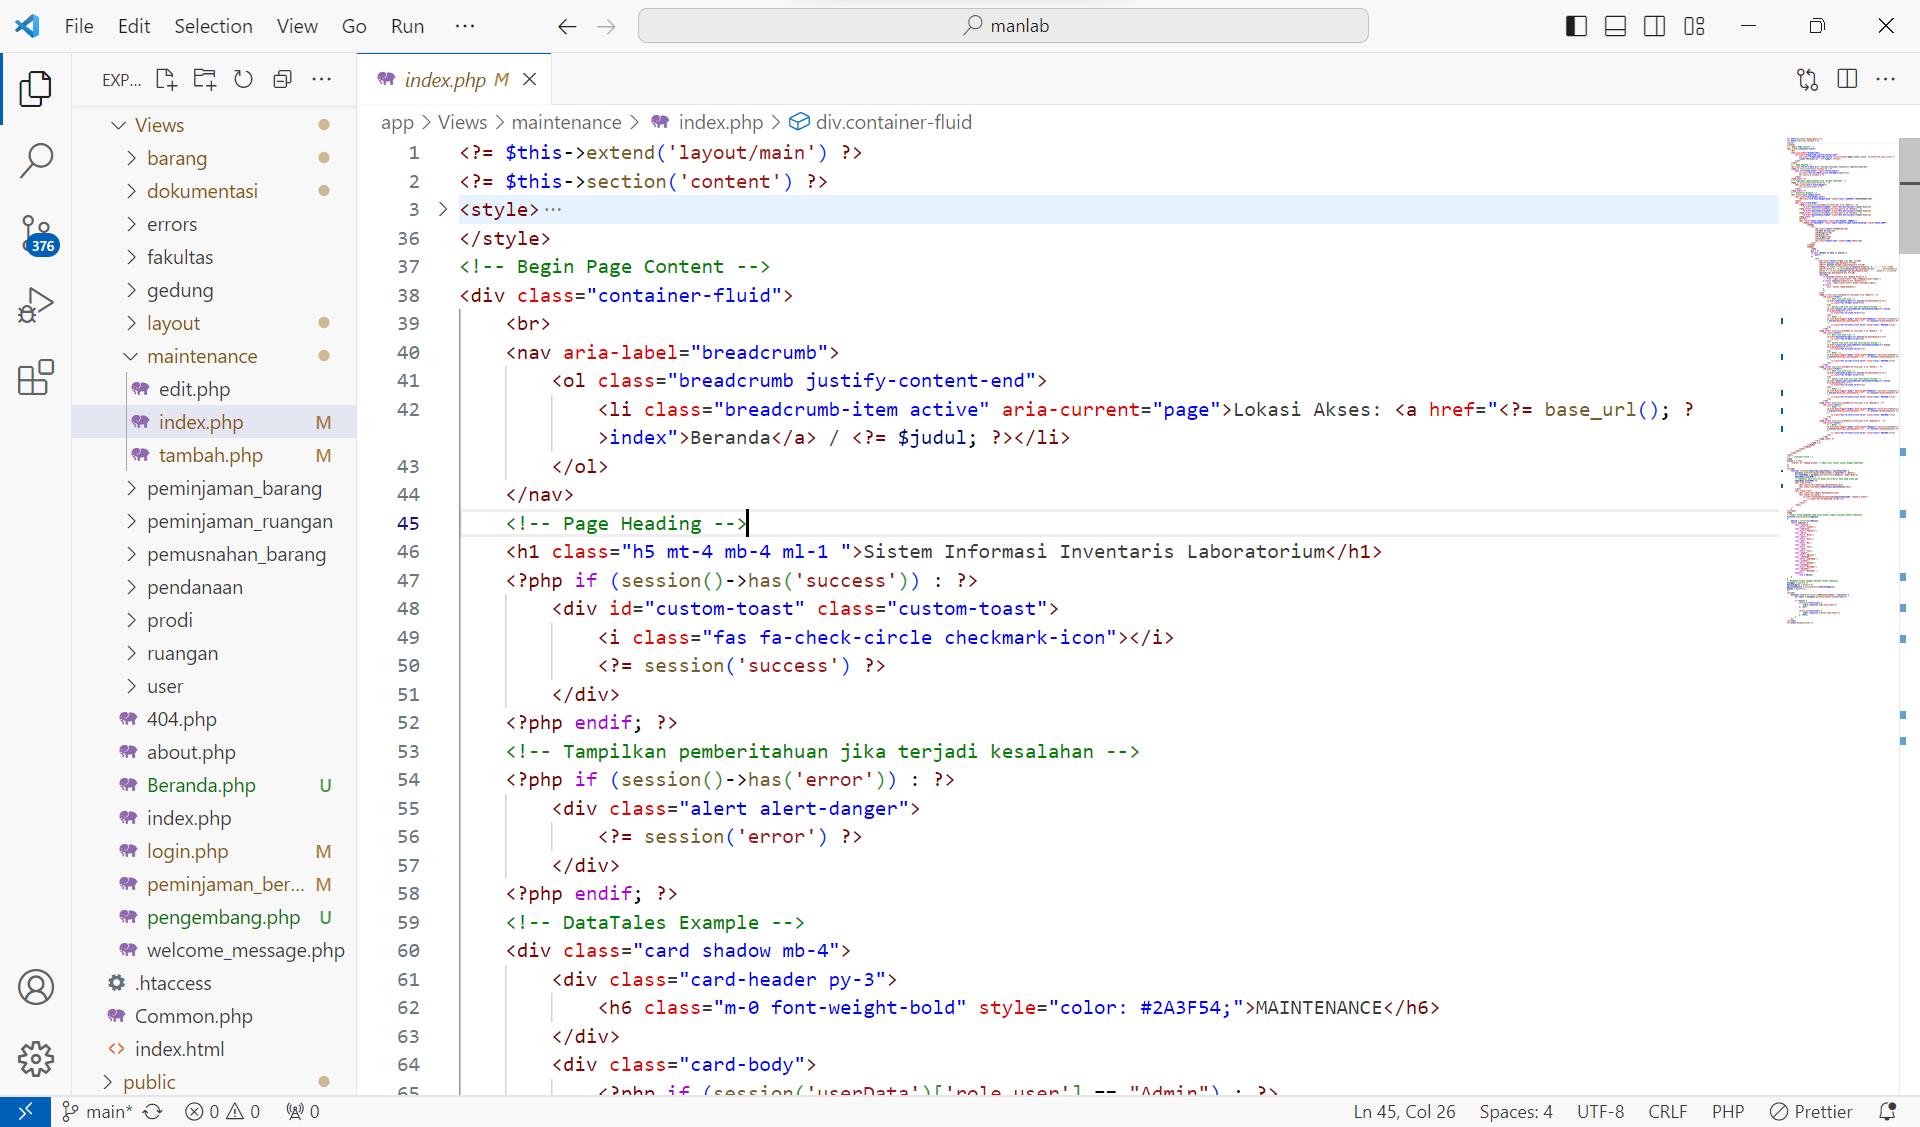
\includegraphics[width=0.82\linewidth]{konten//gambar/view maintenance.png}
          \caption{\textit{View Maintenance}}
          \label{fig:enter-label}
        \end{figure}

  \item \textit{View} dalam implementasi sistem informasi inventaris laboratorium pada data peminjaman barang dapat dilihat pada Gambar 4.45.
        \begin{figure}
          \centering
          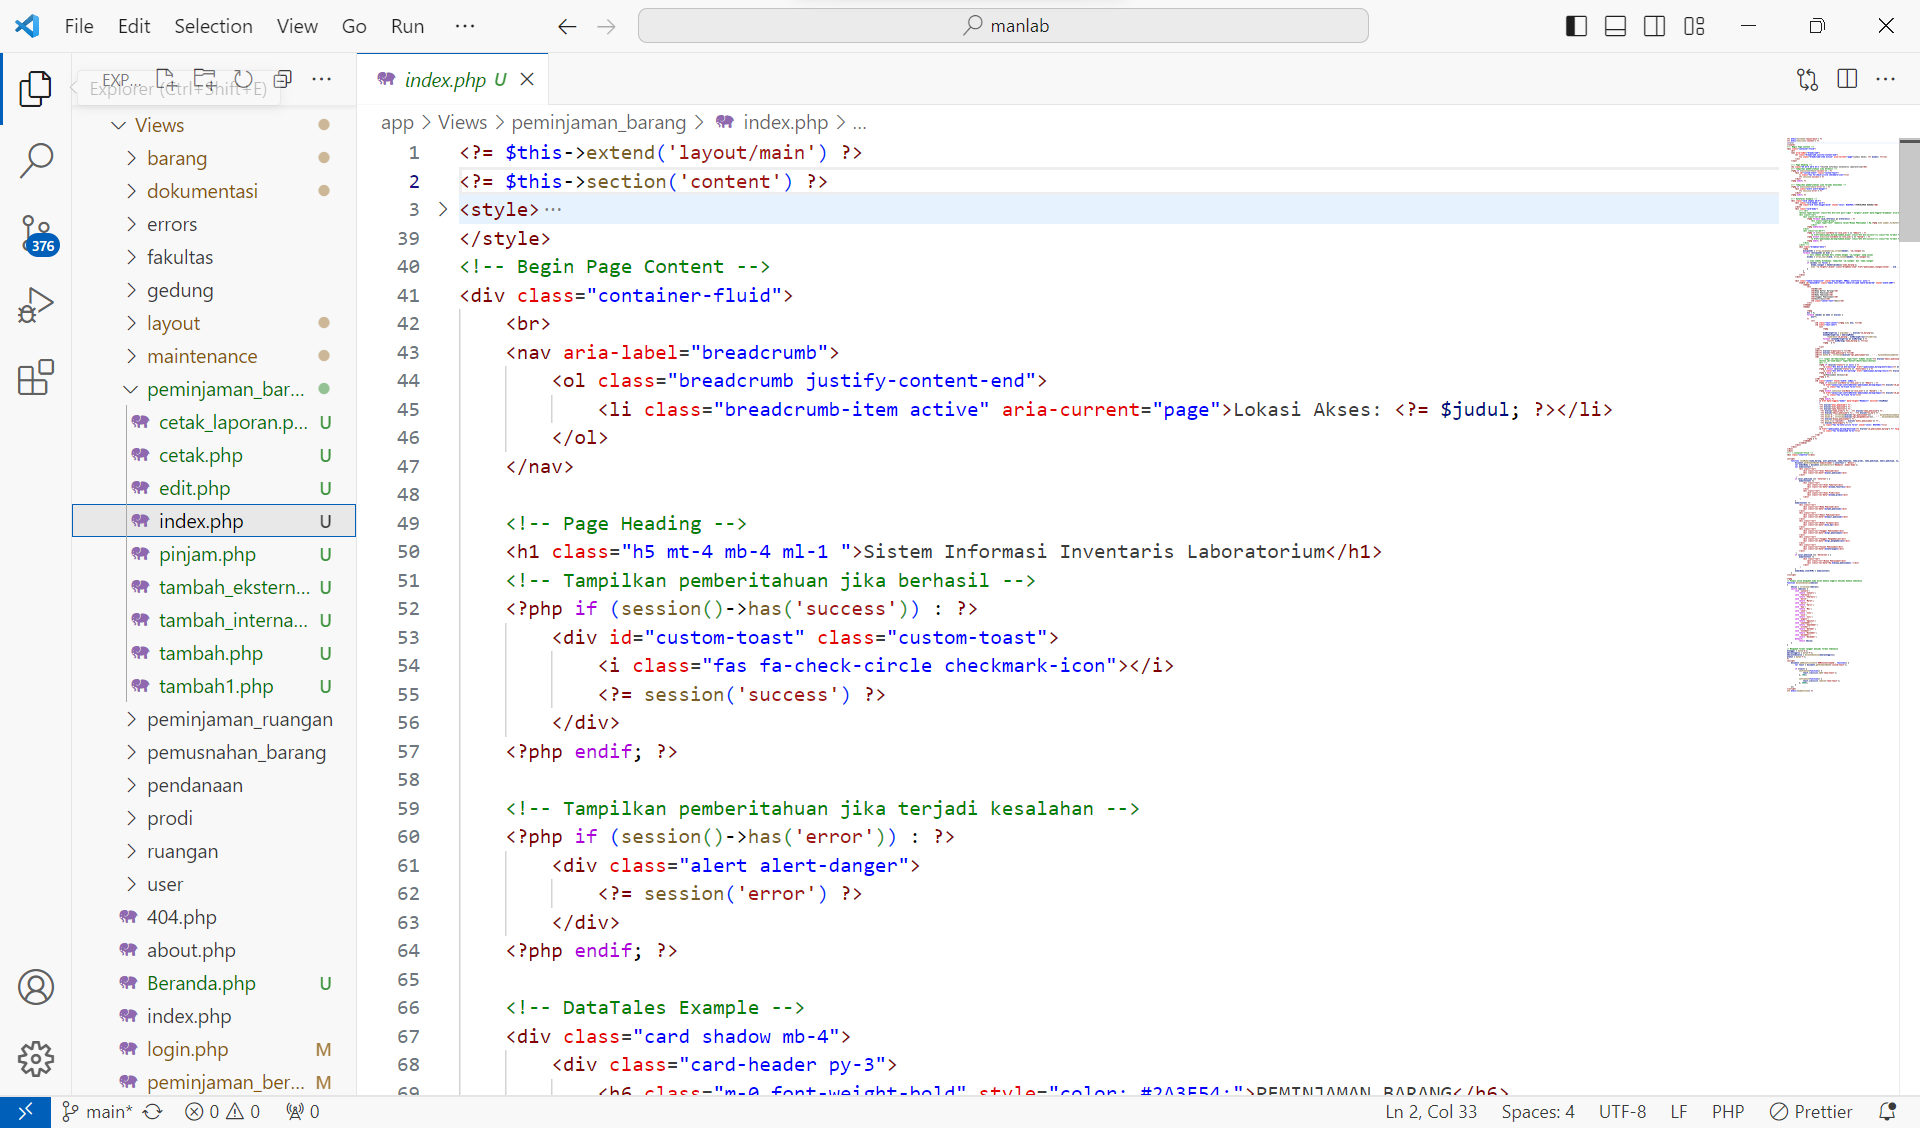
\includegraphics[width=0.82\linewidth]{konten//gambar/view peminjaman_barang.png}
          \caption{\textit{View} Peminjaman Barang}
          \label{fig:enter-label}
        \end{figure}

  \item \textit{View} dalam implementasi sistem informasi inventaris laboratorium pada data peminjaman ruangan dapat dilihat pada Gambar 4.46.
        \begin{figure}
          \centering
          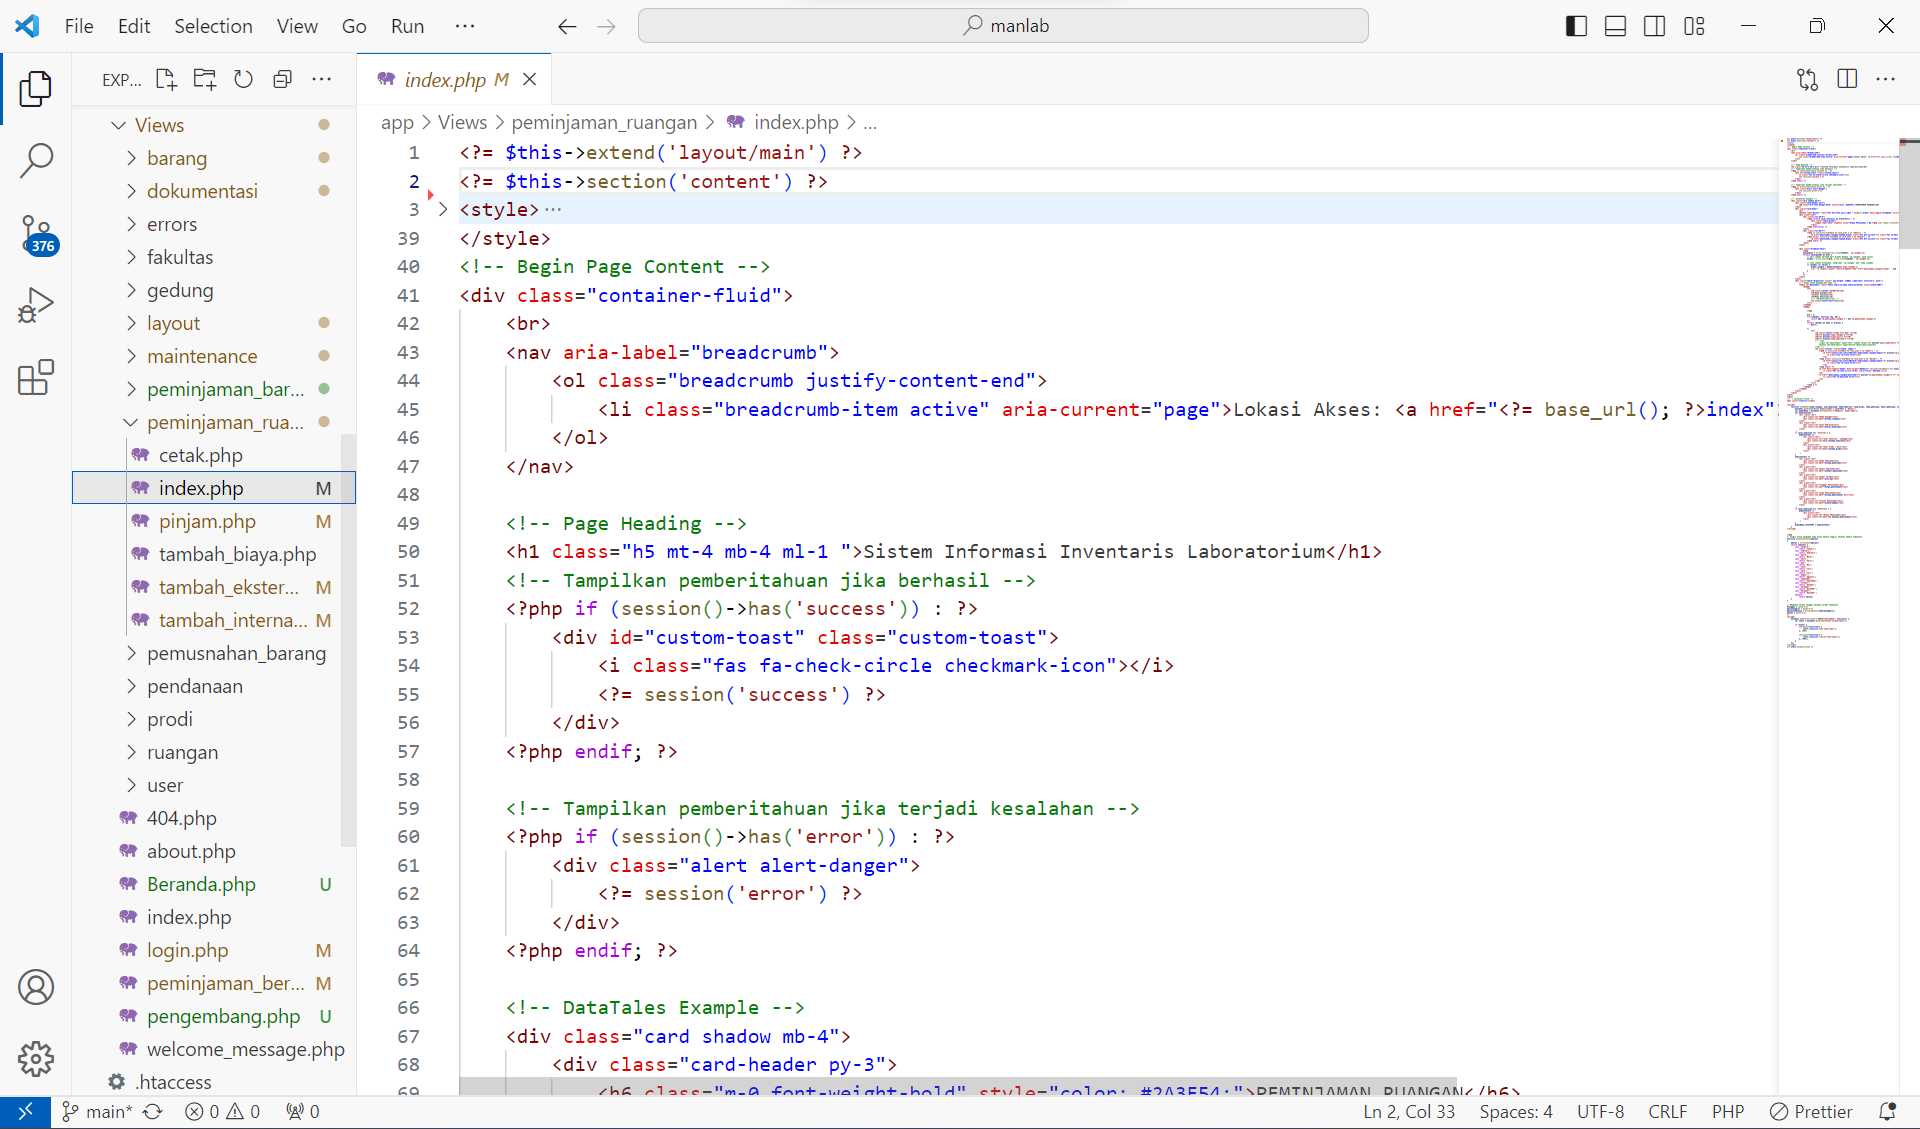
\includegraphics[width=0.82\linewidth]{konten//gambar/view peminjaman_ruangan.png}
          \caption{\textit{View} Peminjaman Ruangan}
          \label{fig:enter-label}
        \end{figure}

  \item \textit{View} dalam implementasi sistem informasi inventaris laboratorium pada data pemusnahan barang dapat dilihat pada Gambar 4.47.
        \begin{figure}
          \centering
          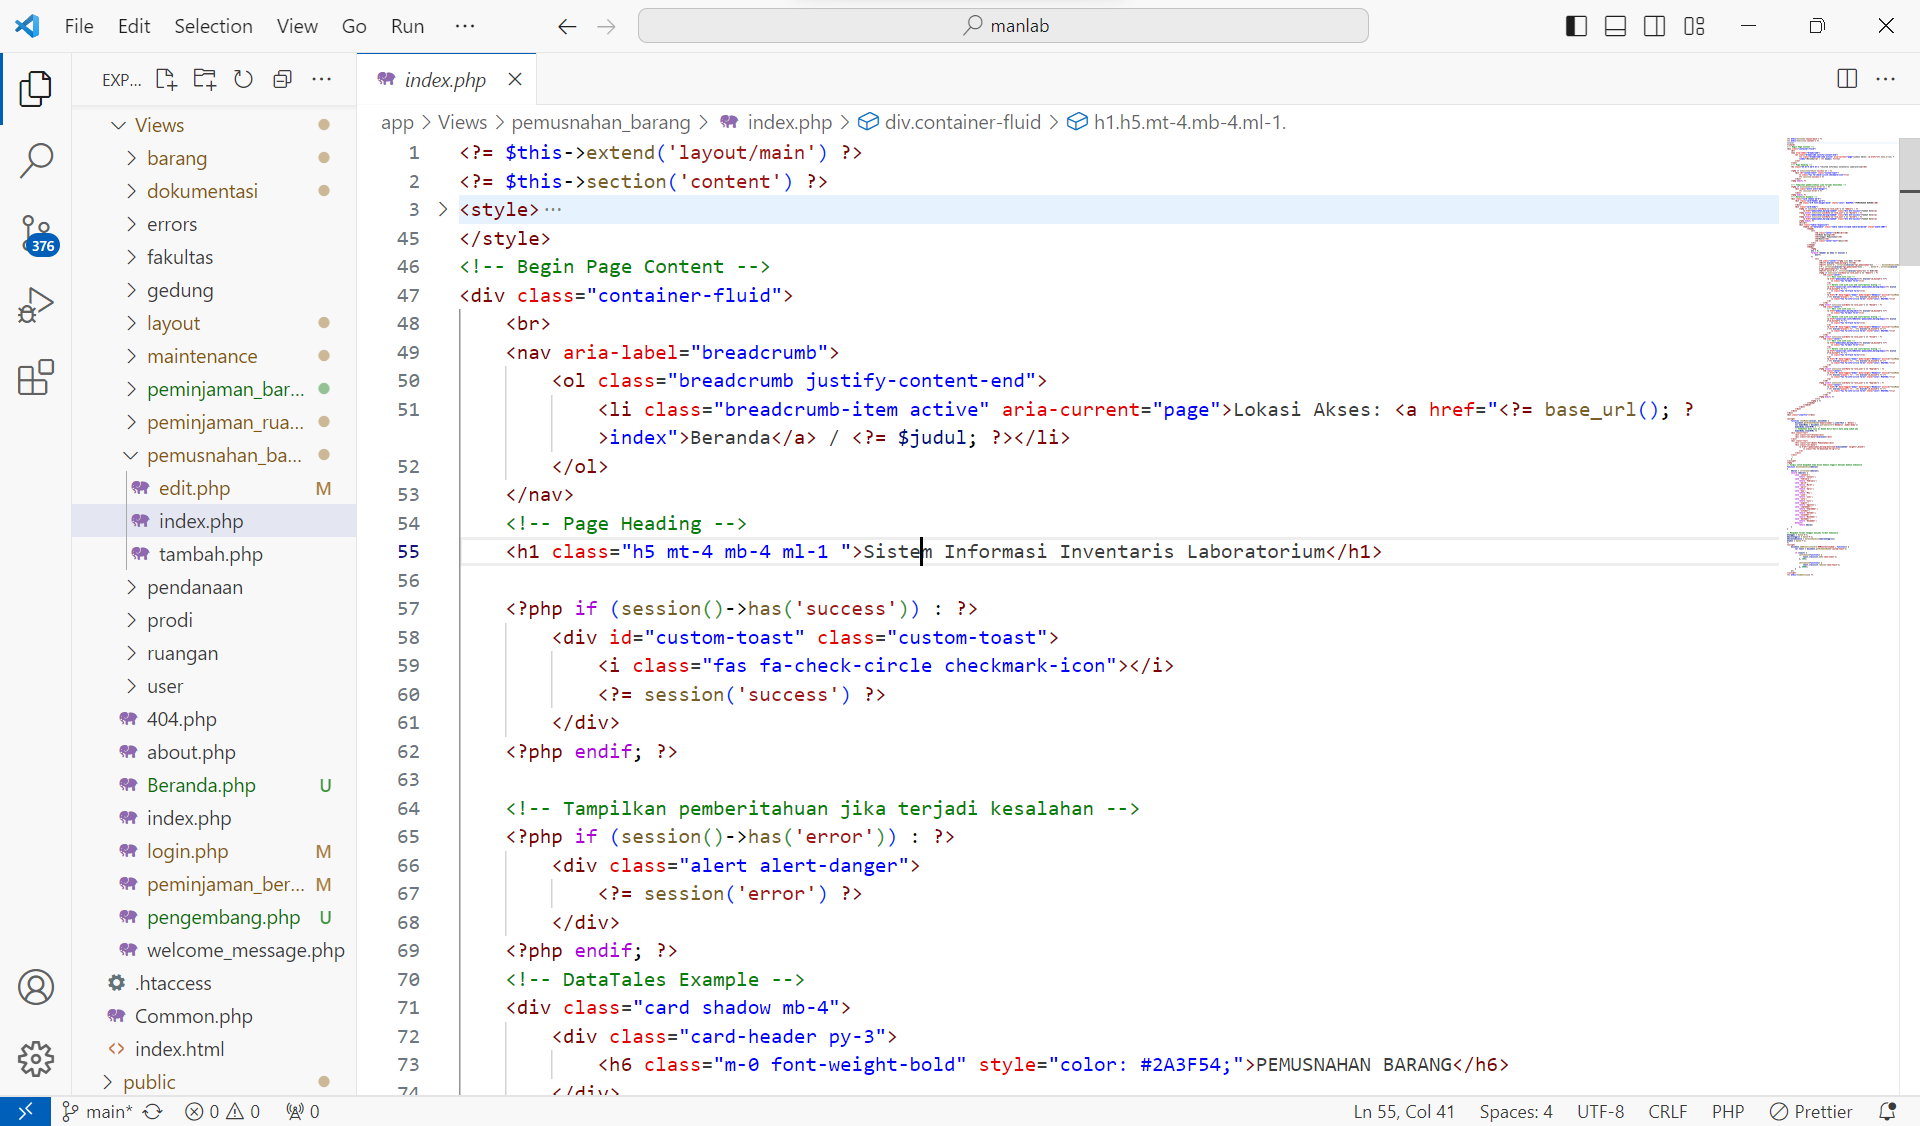
\includegraphics[width=0.82\linewidth]{konten//gambar/view pemusnahan_barang.png}
          \caption{\textit{View} Pemusnahan Barang}
          \label{fig:enter-label}
        \end{figure}

  \item \textit{View} dalam implementasi sistem informasi inventaris laboratorium pada data pendanaan dapat dilihat pada Gambar 4.48.
        \begin{figure}
          \centering
          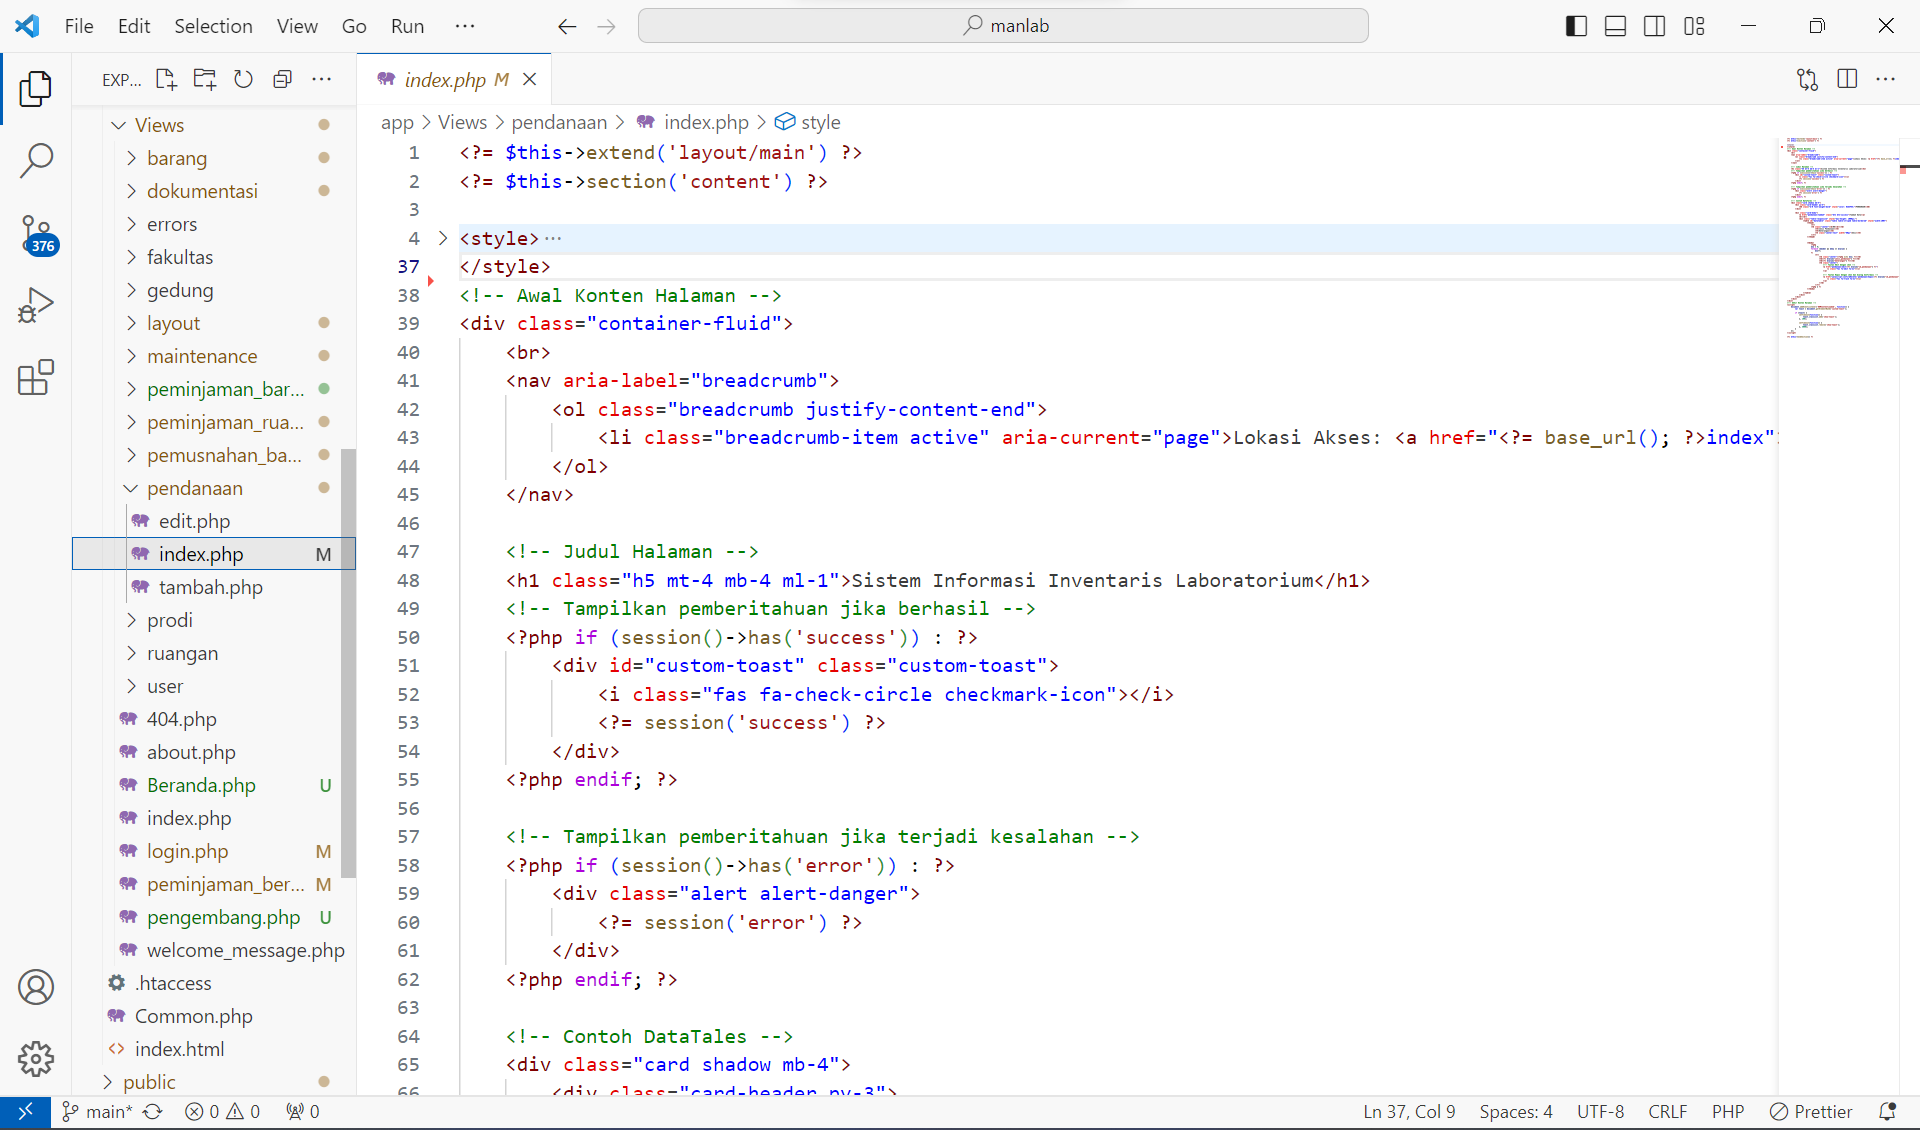
\includegraphics[width=0.82\linewidth]{konten//gambar/view pendanaan.png}
          \caption{\textit{View} Pendanaan}
          \label{fig:enter-label}
        \end{figure}

  \item \textit{View} dalam implementasi sistem informasi inventaris laboratorium pada data prodi dapat dilihat pada Gambar 4.49.
        \begin{figure}
          \centering
          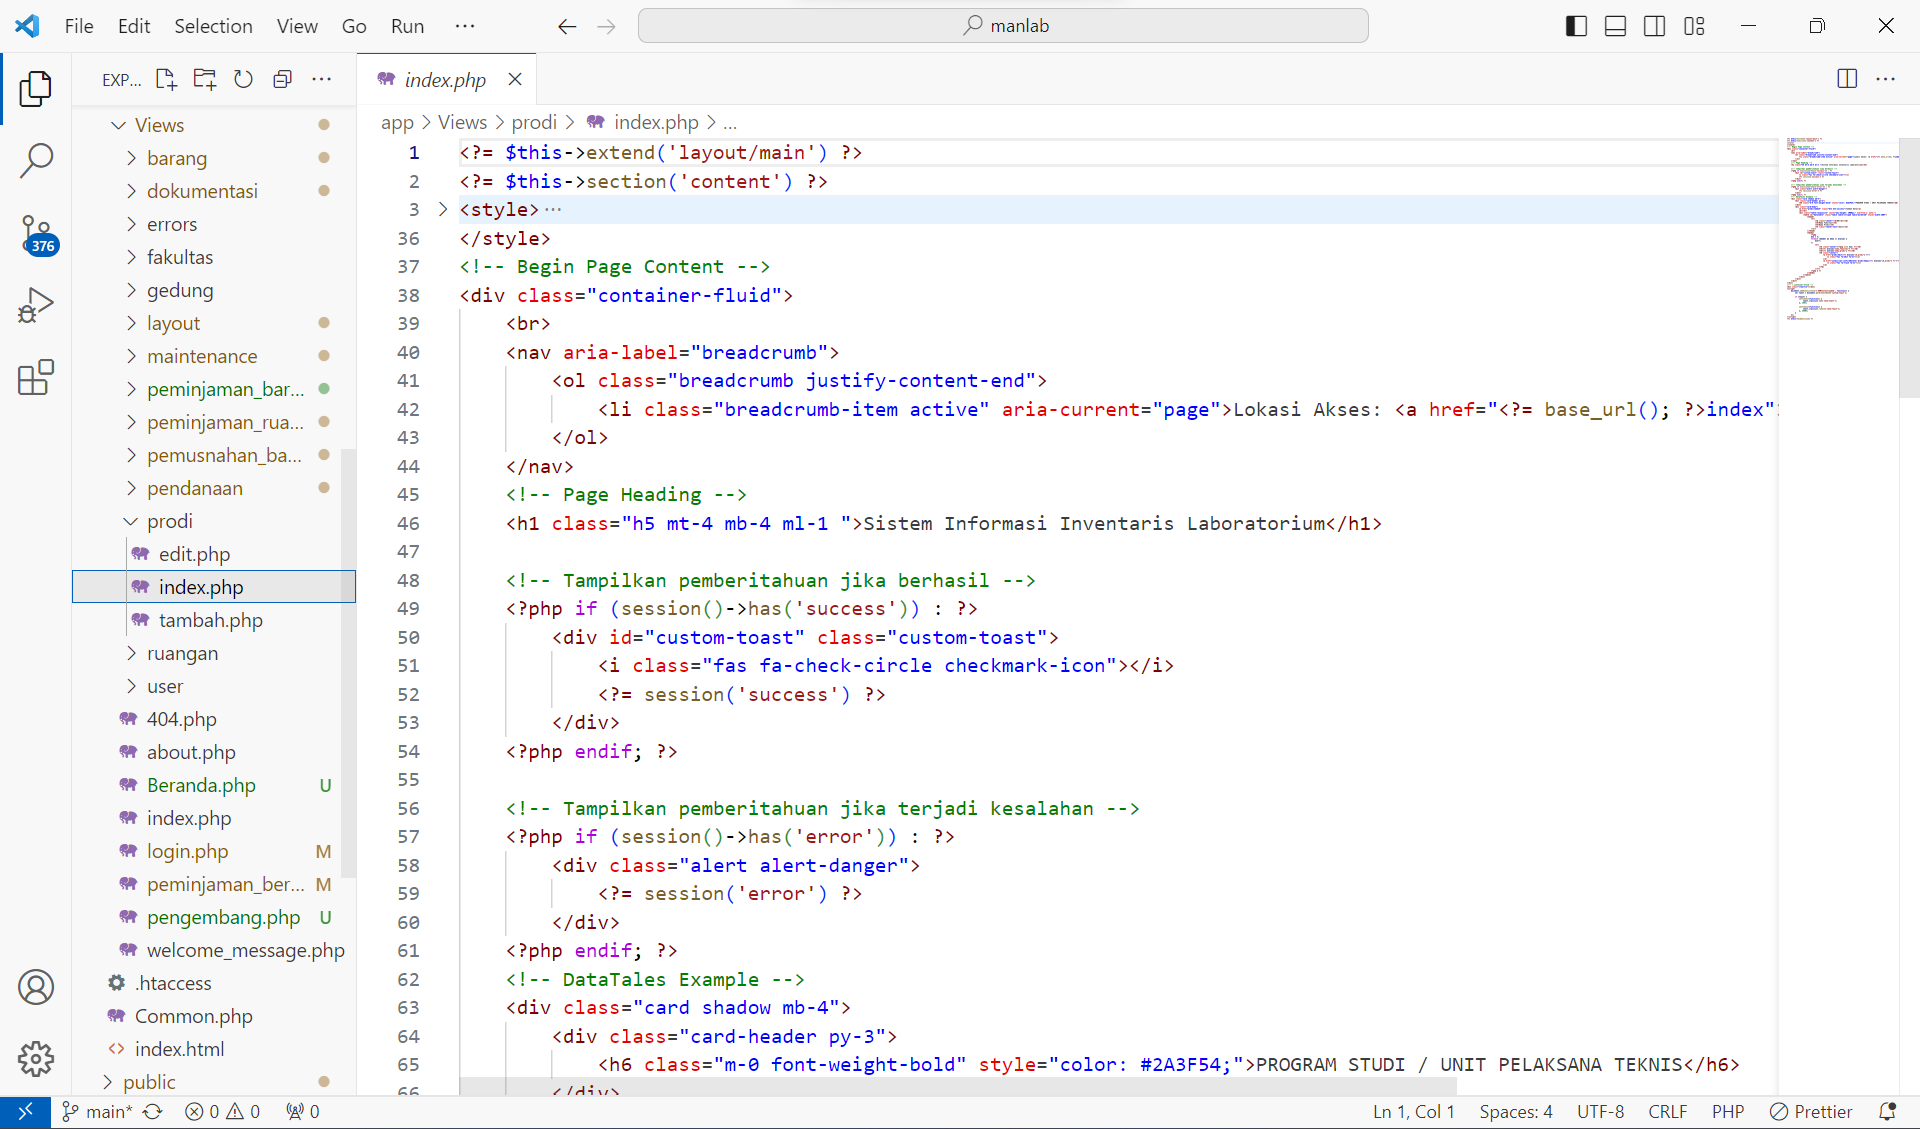
\includegraphics[width=0.82\linewidth]{konten//gambar/view prodi.png}
          \caption{\textit{View} Prodi}
          \label{fig:enter-label}
        \end{figure}

  \item \textit{View} dalam implementasi sistem informasi inventaris laboratorium pada data ruangan dapat dilihat pada Gambar 4.50.
        \begin{figure}
          \centering
          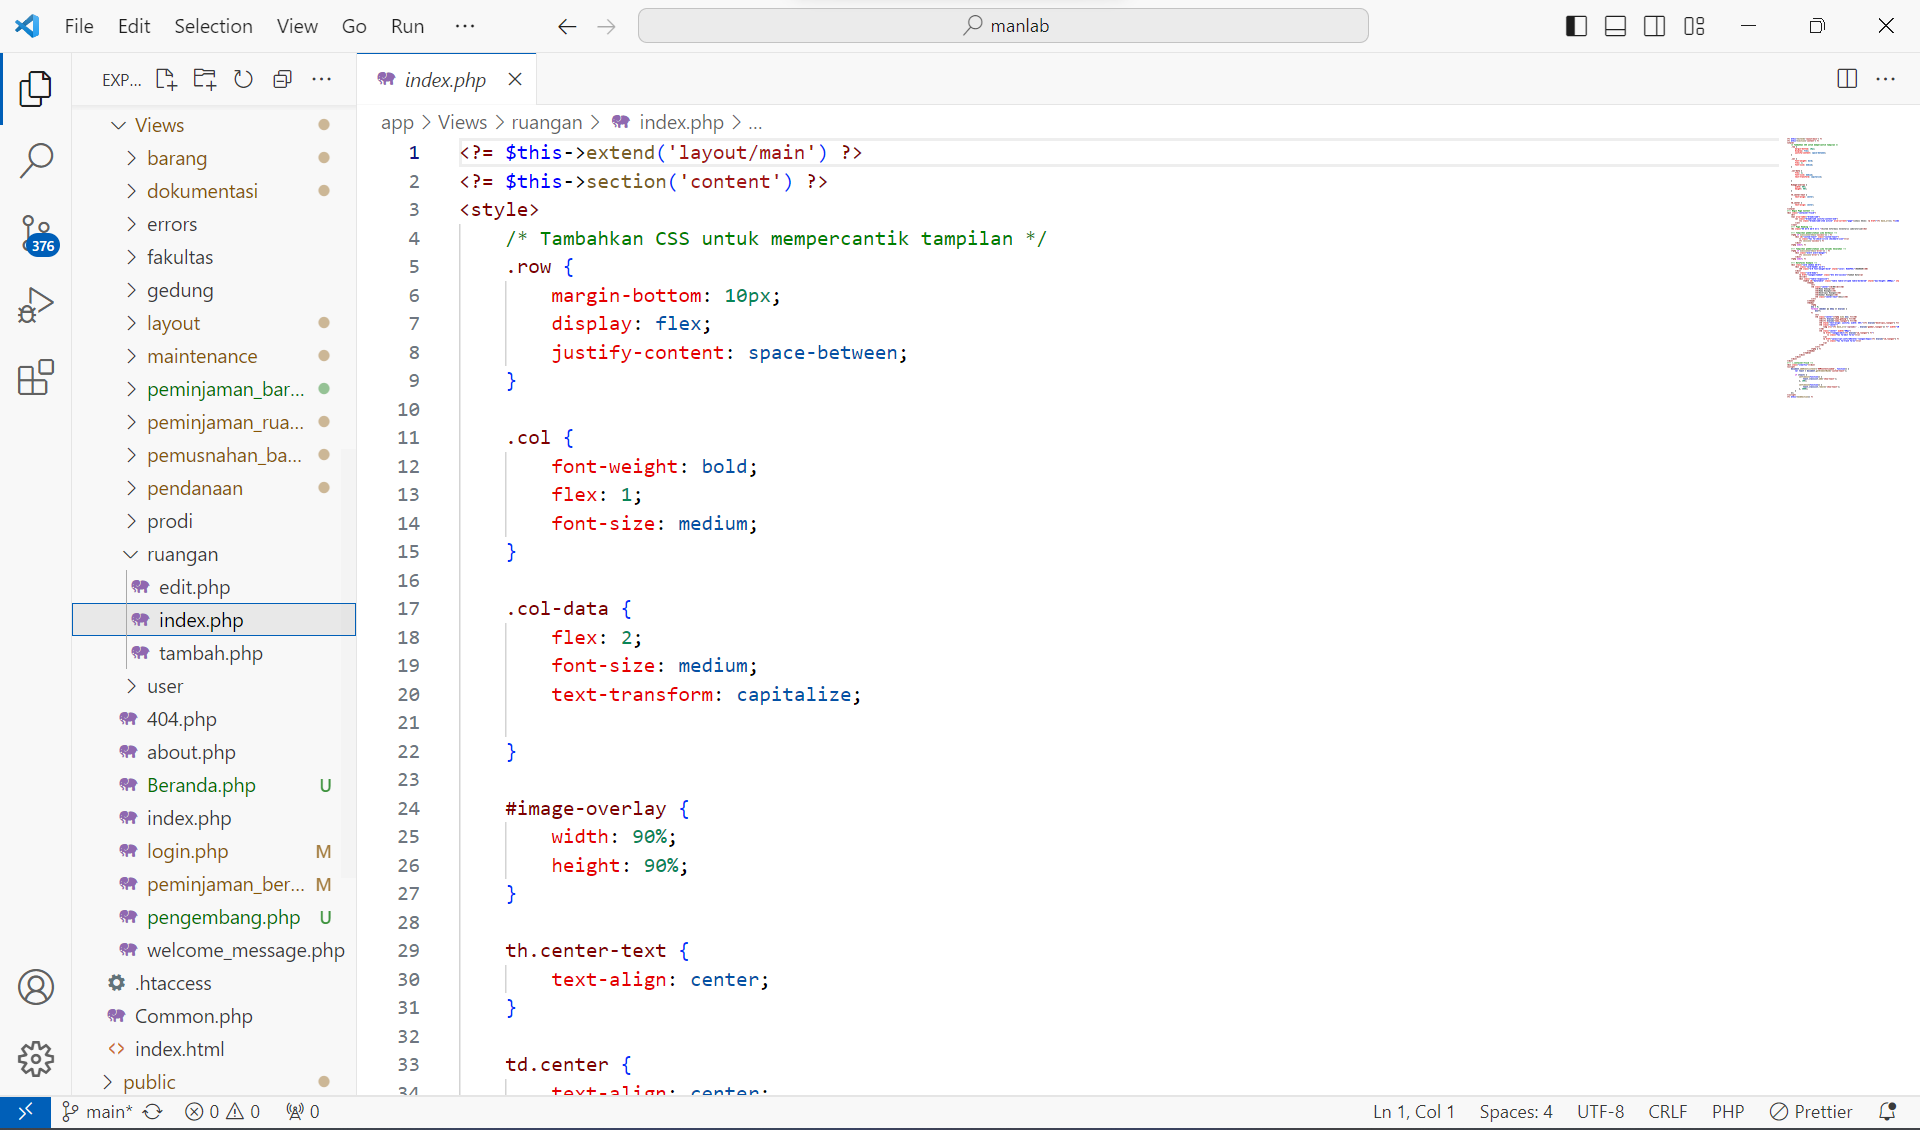
\includegraphics[width=0.82\linewidth]{konten//gambar/view ruangan.png}
          \caption{\textit{View} Ruangan}
          \label{fig:enter-label}
        \end{figure}

  \item \textit{View} dalam implementasi sistem informasi inventaris laboratorium pada data \textit{user} dapat dilihat pada Gambar 4.51.
        \begin{figure}
          \centering
          \includegraphics[width=0.82\linewidth]{konten//gambar/view user.png}
          \caption{\textit{View User}}
          \label{fig:enter-label}
        \end{figure}

\end{enumerate}

\subsection{\textit{Controller}}
\textit{Controller} adalah komponen yang bertanggung jawab untuk mengatur logika pengendalian atau interaksi antara Model (data), \textit{View} (tampilan), dan pengguna \cite{rahman2018perancangan}.

\begin{enumerate}
  \item \textit{Controller} dalam implementasi sistem informasi inventaris laboratorium pada data barang dapat dilihat pada Gambar 4.52.

        \begin{figure}
          \centering
          \includegraphics[width=0.82\linewidth]{konten//gambar/barang controller.png}
          \caption{\textit{Controller} Barang}
          \label{fig:enter-label}
        \end{figure}

  \item \textit{Controller} dalam implementasi sistem informasi inventaris laboratorium pada data dokumentasi dapat dilihat pada Gambar 4.53.

        \begin{figure}
          \centering
          \includegraphics[width=0.82\linewidth]{konten//gambar/dokumentasi controller.png}
          \caption{\textit{Controller} Dokumentasi}
          \label{fig:enter-label}
        \end{figure}

  \item \textit{Controller} dalam implementasi sistem informasi inventaris laboratorium pada data fakultas dapat dilihat pada Gambar 4.54.

        \begin{figure}
          \centering
          \includegraphics[width=0.82\linewidth]{konten//gambar/fakultas controller.png}
          \caption{\textit{Controller} Fakultas}
          \label{fig:enter-label}
        \end{figure}

  \item \textit{Controller} dalam implementasi sistem informasi inventaris laboratorium pada data gedung dapat dilihat pada Gambar 4.55.

        \begin{figure}
          \centering
          \includegraphics[width=0.82\linewidth]{konten//gambar/gedung controller.png}
          \caption{\textit{Controller} Gedung }
          \label{fig:enter-label}
        \end{figure}

  \item \textit{Controller} dalam implementasi sistem informasi inventaris laboratorium pada data \textit{maintenance} dapat dilihat pada Gambar 4.56.

        \begin{figure}
          \centering
          \includegraphics[width=0.82\linewidth]{konten//gambar/maintenance controller.png}
          \caption{\textit{Controller Maintenance}}
          \label{fig:enter-label}
        \end{figure}

  \item \textit{Controller} dalam implementasi sistem informasi inventaris laboratorium pada data peminjaman barang dapat dilihat pada Gambar 4.57.

        \begin{figure}
          \centering
          \includegraphics[width=0.82\linewidth]{konten//gambar/peminjaman barang controller.png}
          \caption{\textit{Controller} Peminjaman Barang}
          \label{fig:enter-label}
        \end{figure}

  \item \textit{Controller} dalam implementasi sistem informasi inventaris laboratorium pada data peminjaman ruangan dapat dilihat pada Gambar 4.58.

        \begin{figure}
          \centering
          \includegraphics[width=0.82\linewidth]{konten//gambar/peminjaman ruangan controller.png}
          \caption{\textit{Controller} Peminjaman Ruangan}
          \label{fig:enter-label}
        \end{figure}

  \item \textit{Controller} dalam implementasi sistem informasi inventaris laboratorium pada data pemusnahan barang dapat dilihat pada Gambar 4.59.

        \begin{figure}
          \centering
          \includegraphics[width=0.82\linewidth]{konten//gambar/pemusnahan barang controller.png}
          \caption{\textit{Controller} Pemusnahan Barang}
          \label{fig:enter-label}
        \end{figure}

  \item \textit{Controller} dalam implementasi sistem informasi inventaris laboratorium pada data pendanaan dapat dilihat pada Gambar 4.60.

        \begin{figure}
          \centering
          \includegraphics[width=0.82\linewidth]{konten//gambar/pendanaan controller.png}
          \caption{\textit{Controller} Pendanaan}
          \label{fig:enter-label}
        \end{figure}

  \item \textit{Controller} dalam implementasi sistem informasi inventaris laboratorium pada data prodi dapat dilihat pada Gambar 4.61.

        \begin{figure}
          \centering
          \includegraphics[width=0.82\linewidth]{konten//gambar/prodi controller.png}
          \caption{\textit{Controller} Prodi}
          \label{fig:enter-label}
        \end{figure}

  \item \textit{Controller} dalam implementasi sistem informasi inventaris laboratorium pada data referensi dapat dilihat pada Gambar 4.62.

        \begin{figure}
          \centering
          \includegraphics[width=0.82\linewidth]{konten//gambar/referensi controller.png}
          \caption{\textit{Controller} Referensi}
          \label{fig:enter-label}
        \end{figure}

  \item \textit{Controller} dalam implementasi sistem informasi inventaris laboratorium pada data ruangan dapat dilihat pada Gambar 4.63.

        \begin{figure}
          \centering
          \includegraphics[width=0.82\linewidth]{konten//gambar/ruangan controller.png}
          \caption{\textit{Controller} Ruangan}
          \label{fig:enter-label}
        \end{figure}

  \item \textit{Controller} dalam implementasi sistem informasi inventaris laboratorium pada data \textit{user} dapat dilihat pada Gambar 4.64.

        \begin{figure}
          \centering
          \includegraphics[width=0.82\linewidth]{konten//gambar/user controller.png}
          \caption{\textit{Controller User}}
          \label{fig:enter-label}
        \end{figure}

\end{enumerate}

% -----------------------------------------------------------------------------%
\section{Hasil Implementasi}

Sistem informasi inventaris yang telah selesai dikembangkan dapat membantu pengguna dalam proses pencatatan aset dan barang. Dengan fitur yang disediakan, diharapkan dapat mempermudah pengguna dalam menggunakan sistem informasi inventaris.

\begin{enumerate}
  \item Halaman \textit{login} \\ Halaman \textit{login} merupakan tampilan awal sistem ketika diakses. Terdapat formulir \textit{username} dan \textit{password} dan dilindungi oleh anti spam dari google reCAPTCHA yang digunakan untuk masuk ke dalam sistem informasi inventaris seperti pada Gambar 4.65.

        \begin{figure}
          \centering
          \includegraphics[width=0.82\linewidth]{konten//gambar/Login Page.png}
          \caption{Halaman \textit{Login}}
          \label{fig:enter-label}
        \end{figure}
        Jika \textit{login} tidak berhasil maka akan menampilkan pesan seperti pada Gambar 4.66.

        \begin{figure}
          \centering
          \includegraphics[width=0.82\linewidth]{konten//gambar/login gagal.png}
          \caption{Tampilan \textit{Login} gagal}
          \label{fig:enter-label}
        \end{figure}

  \item Halaman Beranda \\ Halaman beranda merupakan tampilan awal yang ditampilkan kepada \textit{user} jika \textit{user} berhasil \textit{login} seperti pada Gambar 4.67.

        \begin{figure}
          \centering
          \includegraphics[width=0.82\linewidth]{konten//gambar/login berhasil.png}
          \caption{Halaman Beranda}
          \label{fig:enter-label}
        \end{figure}

        Halaman beranda setiap pengguna berbeda-beda sesuai dengan hak akses yang diberikan, tampilan halaman beranda berdasarkan hak akses seperti pada Gambar 4.68. sampai Gambar 4.72.

        \begin{figure}
          \centering
          \includegraphics[width=0.82\linewidth]{konten//gambar/admin.png}
          \caption{Halaman Beranda Admin}
          \label{fig:enter-label}
        \end{figure}

        \begin{figure}
          \centering
          \includegraphics[width=0.82\linewidth]{konten//gambar/kalab.png}
          \caption{Halaman Beranda Kalab}
          \label{fig:enter-label}
        \end{figure}

        \begin{figure}
          \centering
          \includegraphics[width=0.82\linewidth]{konten//gambar/kaprodi.png}
          \caption{Halaman Beranda Kaprodi}
          \label{fig:enter-label}
        \end{figure}

        \begin{figure}
          \centering
          \includegraphics[width=0.82\linewidth]{konten//gambar/sekprodi.png}
          \caption{Halaman Beranda Sekprodi}
          \label{fig:enter-label}
        \end{figure}

        \begin{figure}
          \centering
          \includegraphics[width=0.82\linewidth]{konten//gambar/aslab.png}
          \caption{Halaman Beranda Aslab}
          \label{fig:enter-label}
        \end{figure}

  \item Halaman Pendanaan \\ Halaman pendanaan merupakan tampilan untuk melihat dan mengelola data pendanaan, tombol tambah data merupakan tombol yang dapat digunakan untuk beralih ke halaman tambah data pendanaan, dan tombol pensil digunakan untuk mengedit data pendanaan dan tombol \textit{trash} untuk menghapus data pendanaan seperti pada Gambar 4.73. sampai Gambar 4.75.

        \begin{figure}
          \centering
          \includegraphics[width=0.82\linewidth]{konten//gambar/pendanaan.png}
          \caption{Halaman Pendanaan \textit{Index}}
          \label{fig:enter-label}
        \end{figure}

        \begin{figure}
          \centering
          \includegraphics[width=0.82\linewidth]{konten//gambar/pendanaan tambah.png}
          \caption{Halaman Tambah Pendanaan}
          \label{fig:enter-label}
        \end{figure}

        \begin{figure}
          \centering
          \includegraphics[width=0.82\linewidth]{konten//gambar/pendanaan edit.png}
          \caption{Halaman Edit Pendanaan}
          \label{fig:enter-label}
        \end{figure}

  \item Halaman Barang \\ Halaman barang merupakan tampilan untuk melihat dan mengelola data barang, tombol tambah data merupakan tombol yang dapat digunakan untuk beralih ke halaman tambah data barang, dan tombol pensil digunakan untuk mengedit data barang dan tombol \textit{trash} untuk menghapus data barang, lalu terdapat juga tombol berwarna biru toska yang dibedakan menjadi beberapa tombol yang bertujuan untuk mencetak dokumen laporan berdasarkan pendanaan, ruangan, kategori, tahun, dan QR seperti pada Gambar 4.76. sampai Gambar 4.88.

        \begin{figure}
          \centering
          \includegraphics[width=0.82\linewidth]{konten//gambar/barang.png}
          \caption{Halaman Barang \textit{Index}}
          \label{fig:enter-label}
        \end{figure}

        \begin{figure}
          \centering
          \includegraphics[width=0.82\linewidth]{konten//gambar/barang tambah.png}
          \caption{Halaman Tambah Barang}
          \label{fig:enter-label}
        \end{figure}

        \begin{figure}
          \centering
          \includegraphics[width=0.82\linewidth]{konten//gambar/barang edit.png}
          \caption{Halaman Edit Barang}
          \label{fig:enter-label}
        \end{figure}

        \begin{figure}
          \centering
          \includegraphics[width=0.82\linewidth]{konten//gambar/barang detail.png}
          \caption{Tampilan Detail Barang}
          \label{fig:enter-label}
        \end{figure}

        \begin{figure}
          \centering
          \includegraphics[width=0.82\linewidth]{konten//gambar/barang cetak pendanaan.png}
          \caption{Tampilan Tombol Cetak Pendanaan}
          \label{fig:enter-label}
        \end{figure}

        \begin{figure}
          \centering
          \includegraphics[width=0.82\linewidth]{konten//gambar/barang cetak ruangan.png}
          \caption{Tampilan Tombol Cetak Ruangan}
          \label{fig:enter-label}
        \end{figure}

        \begin{figure}
          \centering
          \includegraphics[width=0.82\linewidth]{konten//gambar/barang cetak kategori.png}
          \caption{Tampilan Tombol Cetak Kategori}
          \label{fig:enter-label}
        \end{figure}

        \begin{figure}
          \centering
          \includegraphics[width=0.82\linewidth]{konten//gambar/barang cetak tahun.png}
          \caption{Tampilan Tombol Cetak Tahun}
          \label{fig:enter-label}
        \end{figure}

        \begin{figure}
          \centering
          \includegraphics[width=0.82\linewidth]{konten//gambar/barang cetak qr.png}
          \caption{Halaman Cetak QR}
          \label{fig:enter-label}
        \end{figure}

        \begin{figure}
          \centering
          \includegraphics[width=0.82\linewidth]{konten//gambar/barang cetak ruangan pdf.png}
          \caption{Halaman Cetak Ruangan}
          \label{fig:enter-label}
        \end{figure}

        \begin{figure}
          \centering
          \includegraphics[width=0.82\linewidth]{konten//gambar/barang cetak pendanaan pdf.png}
          \caption{Halaman Cetak Pendanaan}
          \label{fig:enter-label}
        \end{figure}

        \begin{figure}
          \centering
          \includegraphics[width=0.82\linewidth]{konten//gambar/barang cetak tahun pdf.png}
          \caption{Halaman Cetak Tahun}
          \label{fig:enter-label}
        \end{figure}

        \begin{figure}
          \centering
          \includegraphics[width=0.82\linewidth]{konten//gambar/barang cetak kategori pdf.png}
          \caption{Halaman Cetak Kategori}
          \label{fig:enter-label}
        \end{figure}

  \item Halaman Posisi Barang \\ Halaman posisi barang merupakan tampilan untuk melihat dan mengelola data barang berdasarkan posisi barang, terdapat tombol berwarna biru toska yang dibedakan menjadi beberapa tombol yang bertujuan untuk mencetak dokumen laporan berdasarkan data ruangan yang sedang ditampilkan, pendanaan, kategori, tahun, dan QR seperti pada Gambar 4.89. sampai Gambar 4.91.

        \begin{figure}
          \centering
          \includegraphics[width=0.82\linewidth]{konten//gambar/rsi.png}
          \caption{Halaman Posisi Barang Labor RSI}
          \label{fig:enter-label}
        \end{figure}

        \begin{figure}
          \centering
          \includegraphics[width=0.82\linewidth]{konten//gambar/se.png}
          \caption{Halaman Posisi Barang Labor SE}
          \label{fig:enter-label}
        \end{figure}

        \begin{figure}
          \centering
          \includegraphics[width=0.82\linewidth]{konten//gambar/int.png}
          \caption{Halaman Posisi Barang Labor INT}
          \label{fig:enter-label}
        \end{figure}

  \item Halaman Peminjaman Barang \\ Halaman peminjaman barang merupakan tampilan untuk melihat dan mengelola data peminjaman barang, tombol \textit{trash} untuk menghapus data peminjaman barang. Lalu ada beberapa tahap yang dilakukan oleh peminjam untuk melakukan peminjaman barang seperti mengisi data peminjaman berdasarkan asal peminjam internal atau eksternal seperti pada Gambar 4.92. sampai Gambar 4.99.

        \begin{figure}
          \centering
          \includegraphics[width=0.82\linewidth]{konten//gambar/peminjaman barang index hasil.png}
          \caption{Halaman Peminjaman Barang \textit{Index}}
          \label{fig:enter-label}
        \end{figure}

        %   \begin{figure}
        %       \centering
        %       \includegraphics[width=0.82\linewidth]{konten//gambar/tambah biaya peminjaman ruangan.png}
        %       \caption{Halaman Tambah Biaya Peminjaman Ruangan}
        %       \label{fig:enter-label}
        %   \end{figure}

        \begin{figure}
          \centering
          \includegraphics[width=0.82\linewidth]{konten//gambar/peminjaman barang pinjam hasil.png}
          \caption{Halaman Peminjaman Barang Bagi Peminjam}
          \label{fig:enter-label}
        \end{figure}

        \begin{figure}
          \centering
          \includegraphics[width=0.82\linewidth]{konten//gambar/peminjaman barang tambah internal 1 hasil.png}
          \caption{Halaman Peminjaman Barang Bagi Peminjam Internal Tahap 1}
          \label{fig:enter-label}
        \end{figure}

        \begin{figure}
          \centering
          \includegraphics[width=0.82\linewidth]{konten//gambar/peminjaman barang tambah internal 2 hasil.png}
          \caption{Halaman Peminjaman Barang Bagi Peminjam Internal Tahap 2}
          \label{fig:enter-label}
        \end{figure}

        \begin{figure}
          \centering
          \includegraphics[width=0.82\linewidth]{konten//gambar/peminjaman barang tambah internal 3 hasil.png}
          \caption{Halaman Peminjaman Barang Bagi Peminjam Internal Tahap 3}
          \label{fig:enter-label}
        \end{figure}

        \begin{figure}
          \centering
          \includegraphics[width=0.82\linewidth]{konten//gambar/peminjaman barang tambah eksternal 1 hasil.png}
          \caption{Halaman Peminjaman Barang Bagi Peminjam Eksternal Tahap 1}
          \label{fig:enter-label}
        \end{figure}

        \begin{figure}
          \centering
          \includegraphics[width=0.82\linewidth]{konten//gambar/peminjaman barang tambah eksternal 2 hasil.png}
          \caption{Halaman Peminjaman Barang Bagi Peminjam Eksternal Tahap 2}
          \label{fig:enter-label}
        \end{figure}

        \begin{figure}
          \centering
          \includegraphics[width=0.82\linewidth]{konten//gambar/peminjaman barang tambah eksternal 3 hasil.png}
          \caption{Halaman Peminjaman Barang Bagi Peminjam Eksternal Tahap 3}
          \label{fig:enter-label}
        \end{figure}

  \item Halaman Peminjaman Ruangan \\ Halaman peminjaman ruangan merupakan tampilan untuk melihat dan mengelola data peminjaman ruangan, tombol \textit{trash} untuk menghapus data peminjaman ruangan. Lalu ada beberapa tahap yang dilakukan oleh peminjam untuk melakukan peminjaman ruangan seperti mengisi data peminjaman berdasarkan asal peminjam internal atau eksternal seperti pada Gambar 4.100. sampai Gambar 4.104.

        \begin{figure}
          \centering
          \includegraphics[width=0.82\linewidth]{konten//gambar/peminjaman ruangan index.png}
          \caption{Halaman Peminjaman Ruangan \textit{Index}}
          \label{fig:enter-label}
        \end{figure}

        \begin{figure}
          \centering
          \includegraphics[width=0.82\linewidth]{konten//gambar/tambah biaya peminjaman ruangan.png}
          \caption{Halaman Tambah Biaya Peminjaman Ruangan}
          \label{fig:enter-label}
        \end{figure}

        \begin{figure}
          \centering
          \includegraphics[width=0.82\linewidth]{konten//gambar/peminjaman ruangan peminjam.png}
          \caption{Halaman Peminjaman Ruangan Bagi Peminjam}
          \label{fig:enter-label}
        \end{figure}

        \begin{figure}
          \centering
          \includegraphics[width=0.82\linewidth]{konten//gambar/peminjaman ruangan tambah internal.png}
          \caption{Halaman Peminjaman Ruangan Bagi Peminjam Internal}
          \label{fig:enter-label}
        \end{figure}

        \begin{figure}
          \centering
          \includegraphics[width=0.82\linewidth]{konten//gambar/peminjaman ruangan tambah eksternal.png}
          \caption{Halaman Peminjaman Ruangan Bagi Peminjam Eksternal}
          \label{fig:enter-label}
        \end{figure}

  \item Halaman Dokumentasi \\ Halaman dokumentasi merupakan tampilan untuk melihat dan mengelola data dokumentasi, tombol tambah data merupakan tombol yang dapat digunakan untuk beralih ke halaman tambah data dokumentasi, dan tombol pensil digunakan untuk mengedit data dokumentasi dan tombol \textit{trash} untuk menghapus data dokumentasi seperti pada Gambar 4.105. sampai Gambar 4.109.

        \begin{figure}
          \centering
          \includegraphics[width=0.82\linewidth]{konten//gambar/dokumentasi index.png}
          \caption{Halaman Dokumentasi \textit{Index}}
          \label{fig:enter-label}
        \end{figure}

        \begin{figure}
          \centering
          \includegraphics[width=0.82\linewidth]{konten//gambar/dokumentasi detail.png}
          \caption{Tampilan Detail Dokumentasi}
          \label{fig:enter-label}
        \end{figure}

        \begin{figure}
          \centering
          \includegraphics[width=0.82\linewidth]{konten//gambar/dokumentasi tambah.png}
          \caption{Halaman Tambah Dokumentasi}
          \label{fig:enter-label}
        \end{figure}

        \begin{figure}
          \centering
          \includegraphics[width=0.82\linewidth]{konten//gambar/dokumentasi edit.png}
          \caption{Halaman Edit Dokumentasi}
          \label{fig:enter-label}
        \end{figure}

        \begin{figure}
          \centering
          \includegraphics[width=0.82\linewidth]{konten//gambar/dokumentasi download.png}
          \caption{Halaman Download Dokumentasi}
          \label{fig:enter-label}
        \end{figure}

  \item Halaman \textit{Maintenance} \\ Halaman \textit{maintenance} merupakan tampilan untuk melihat dan mengelola data \textit{maintenance}, tombol tambah data merupakan tombol yang dapat digunakan untuk beralih ke halaman tambah data \textit{maintenance}, dan tombol pensil digunakan untuk mengedit data \textit{maintenance} dan tombol \textit{trash} untuk menghapus data \textit{maintenance} seperti pada Gambar 4.110. sampai Gambar 4.113.
        \begin{figure}
          \centering
          \includegraphics[width=0.82\linewidth]{konten//gambar/maintenance index.png}
          \caption{Halaman \textit{Maintenance} \textit{Index}}
          \label{fig:enter-label}
        \end{figure}

        \begin{figure}
          \centering
          \includegraphics[width=0.82\linewidth]{konten//gambar/maintenance detail.png}
          \caption{Tampilan Detail \textit{Maintenance}}
          \label{fig:enter-label}
        \end{figure}

        \begin{figure}
          \centering
          \includegraphics[width=0.82\linewidth]{konten//gambar/maintenance tambah.png}
          \caption{Halaman Tambah \textit{Maintenance}}
          \label{fig:enter-label}
        \end{figure}

        \begin{figure}
          \centering
          \includegraphics[width=0.82\linewidth]{konten//gambar/maintenance edit.png}
          \caption{Halaman Edit \textit{Maintenance}}
          \label{fig:enter-label}
        \end{figure}

  \item Halaman Pemusnahan Barang \\ Halaman pemusnahan barang merupakan tampilan untuk melihat dan mengelola data pemusnahan barang, tombol tambah data merupakan tombol yang dapat digunakan untuk beralih ke halaman tambah data pemusnahan barang, dan tombol pensil digunakan untuk mengedit data pemusnahan barang dan tombol \textit{trash} untuk menghapus data pemusnahan barang seperti pada Gambar 4.114. sampai Gambar 4.117.

        \begin{figure}
          \centering
          \includegraphics[width=0.82\linewidth]{konten//gambar/pemusnahan barang index.png}
          \caption{Halaman Pemusnahan Barang \textit{Index}}
          \label{fig:enter-label}
        \end{figure}

        \begin{figure}
          \centering
          \includegraphics[width=0.82\linewidth]{konten//gambar/pemusnahan barangdtl.png}
          \caption{Tampilan Detail Pemusnahan Barang}
          \label{fig:enter-label}
        \end{figure}

        \begin{figure}
          \centering
          \includegraphics[width=0.82\linewidth]{konten//gambar/pemusnahan barangtbh.png}
          \caption{Halaman Tambah Pemusnahan Barang}
          \label{fig:enter-label}
        \end{figure}

        \begin{figure}
          \centering
          \includegraphics[width=0.82\linewidth]{konten//gambar/pemusnahan barang edit.png}
          \caption{Halaman Edit Pemusnahan Barang}
          \label{fig:enter-label}
        \end{figure}

  \item Halaman Fakultas \\ Halaman fakultas merupakan tampilan untuk melihat dan mengelola data fakultas, tombol tambah data merupakan tombol yang dapat digunakan untuk beralih ke halaman tambah data fakultas, dan tombol pensil digunakan untuk mengedit data fakultas dan tombol \textit{trash} untuk menghapus data fakultas seperti pada Gambar 4.118. sampai Gambar 4.120.

        \begin{figure}
          \centering
          \includegraphics[width=0.82\linewidth]{konten//gambar/fakultas index.png}
          \caption{Halaman Fakultas \textit{Index}}
          \label{fig:enter-label}
        \end{figure}

        \begin{figure}
          \centering
          \includegraphics[width=0.82\linewidth]{konten//gambar/fakultas tambah.png}
          \caption{Halaman Tambah Fakultas}
          \label{fig:enter-label}
        \end{figure}

        \begin{figure}
          \centering
          \includegraphics[width=0.82\linewidth]{konten//gambar/fakultas edit.png}
          \caption{Halaman Edit Fakultas}
          \label{fig:enter-label}
        \end{figure}

  \item Halaman Prodi \\ Halaman prodi merupakan tampilan untuk melihat dan mengelola data prodi, tombol tambah data merupakan tombol yang dapat digunakan untuk beralih ke halaman tambah data prodi, dan tombol pensil digunakan untuk mengedit data prodi dan tombol \textit{trash} untuk menghapus data prodi seperti pada Gambar 4.121. sampai Gambar 4.123.

        \begin{figure}
          \centering
          \includegraphics[width=0.82\linewidth]{konten//gambar/prodi index.png}
          \caption{Halaman Prodi Index}
          \label{fig:enter-label}
        \end{figure}

        \begin{figure}
          \centering
          \includegraphics[width=0.82\linewidth]{konten//gambar/prodi tambah.png}
          \caption{Halaman Tambah Prodi}
          \label{fig:enter-label}
        \end{figure}

        \begin{figure}
          \centering
          \includegraphics[width=0.82\linewidth]{konten//gambar/prodi edit.png}
          \caption{Halaman Edit Prodi}
          \label{fig:enter-label}
        \end{figure}

  \item Halaman Gedung \\ Halaman gedung merupakan tampilan untuk melihat dan mengelola data gedung, tombol tambah data merupakan tombol yang dapat digunakan untuk beralih ke halaman tambah data gedung, dan tombol pensil digunakan untuk mengedit data gedung dan tombol \textit{trash} untuk menghapus data gedung seperti pada Gambar 4.124. sampai Gambar 4.126.
        \begin{figure}
          \centering
          \includegraphics[width=0.82\linewidth]{konten//gambar/gedung index.png}
          \caption{Halaman Gedung \textit{Index}}
          \label{fig:enter-label}
        \end{figure}

        \begin{figure}
          \centering
          \includegraphics[width=0.82\linewidth]{konten//gambar/gedung tambah.png}
          \caption{Halaman Tambah Gedung}
          \label{fig:enter-label}
        \end{figure}

        \begin{figure}
          \centering
          \includegraphics[width=0.82\linewidth]{konten//gambar/gedung edit.png}
          \caption{Halaman Edit Gedung}
          \label{fig:enter-label}
        \end{figure}

  \item Halaman Ruangan \\ Halaman ruangan merupakan tampilan untuk melihat dan mengelola data ruangan, tombol tambah data merupakan tombol yang dapat digunakan untuk beralih ke halaman tambah data ruangan, dan tombol pensil digunakan untuk mengedit data ruangan dan tombol \textit{trash} untuk menghapus data ruangan seperti pada Gambar 4.127. sampai Gambar 4.129.
        \begin{figure}
          \centering
          \includegraphics[width=0.82\linewidth]{konten//gambar/ruangan index.png}
          \caption{Halaman Ruangan \textit{Index}}
          \label{fig:enter-label}
        \end{figure}

        \begin{figure}
          \centering
          \includegraphics[width=0.82\linewidth]{konten//gambar/ruangan tambah.png}
          \caption{Halaman Tambah Ruangan}
          \label{fig:enter-label}
        \end{figure}

        \begin{figure}
          \centering
          \includegraphics[width=0.82\linewidth]{konten//gambar/ruangan edit.png}
          \caption{Halaman Edit Ruangan}
          \label{fig:enter-label}
        \end{figure}

  \item Halaman Pengguna \\ Halaman pengguna merupakan tampilan untuk melihat dan mengelola data pengguna, tombol tambah data merupakan tombol yang dapat digunakan untuk beralih ke halaman tambah data pengguna, dan tombol pensil digunakan untuk mengedit data pengguna dan tombol \textit{trash} untuk menghapus data pengguna seperti pada Gambar 4.130. sampai Gambar 4.133.

        \begin{figure}
          \centering
          \includegraphics[width=0.82\linewidth]{konten//gambar/user index.png}
          \caption{Halaman Pengguna \textit{Index}}
          \label{fig:enter-label}
        \end{figure}

        \begin{figure}
          \centering
          \includegraphics[width=0.82\linewidth]{konten//gambar/user detail.png}
          \caption{Tampilan Detail Pengguna}
          \label{fig:enter-label}
        \end{figure}

        \begin{figure}
          \centering
          \includegraphics[width=0.82\linewidth]{konten//gambar/user tambah.png}
          \caption{Halaman Tambah Pengguna}
          \label{fig:enter-label}
        \end{figure}

        \begin{figure}
          \centering
          \includegraphics[width=0.82\linewidth]{konten//gambar/user edit.png}
          \caption{Halaman Edit Pengguna}
          \label{fig:enter-label}
        \end{figure}

  \item Halaman Profil \\ Halaman profil merupakan tampilan untuk melihat dan mengelola data profil, tombol edit profil merupakan tombol yang dapat digunakan untuk beralih ke halaman tambah edit profil seperti pada Gambar 4.134. sampai Gambar 4.135.

        \begin{figure}
          \centering
          \includegraphics[width=0.82\linewidth]{konten//gambar/profil.png}
          \caption{Halaman Profil Pengguna}
          \label{fig:enter-label}
        \end{figure}

        \begin{figure}
          \centering
          \includegraphics[width=0.82\linewidth]{konten//gambar/profil edit.png}
          \caption{Halaman Edit Profil Pengguna}
          \label{fig:enter-label}
        \end{figure}

  \item Halaman Pengembang \\ Halaman pengembang merupakan tampilan untuk melihat data pengembang seperti pada Gambar 4.89.

        \begin{figure}
          \centering
          \includegraphics[width=0.82\linewidth]{konten//gambar/pengembang.png}
          \caption{Halaman Pengembang}
          \label{fig:enter-label}
        \end{figure}

\end{enumerate}
% -----------------------------------------------------------------------------%